% --- Set document class and font size ---

\documentclass[12pt]{article}

% --- Package imports ---
% ------------------ MINIMAL WORKING PAPER ------------------
\usepackage[english]{babel}

\usepackage{amsmath,amsfonts,amsthm,amssymb,mathtools} % Mathematical

\usepackage[dvipsnames]{xcolor}
\usepackage{etoolbox} 
\usepackage{tikz} % Drawings
  \usetikzlibrary{3d}
\usepackage{pgfplots} %Pode plotar
  \pgfplotsset{compat=newest}
  \usepgfplotslibrary{fillbetween}
\usepackage{float} 
\usepackage{multirow} 

% ------------------ EXTRA BUT USEFUL ------------------
\usepackage{optidef} 
\usepackage{blindtext} 

\usepackage{hyperref,theoremref} 
\hypersetup{
    pdftitle={PS - Nícolas},
    colorlinks=true, linkcolor=blue!90,
    bookmarksnumbered=true,
    bookmarksopen=true
}

\usepackage{listings}


\usepackage{hyperref}
\usepackage{dcolumn}
\usepackage{footnote}
\usepackage{ulem}
\usepackage{pdfpages}
\usepackage{graphicx}

% ------------------ EXTRA FOR LECTURE NOTES ------------------
\usepackage{
  dsfont, units,          % Math typesetting
  wrapfig,                            % Figures and graphics formatting
  color, inconsolata, pythonhighlight,               % Code formatting
  fancyhdr, sectsty, enumerate, enumitem, framed }   % Headers/footers, section fonts, links, lists

% lipsum is just for generating placeholder text and can be removed
\usepackage{hyperref, lipsum} 


\usepackage{newpxtext, newpxmath, inconsolata}
\usepackage{natbib}
\usepackage{subcaption}

% ------------------ LETTERFONTS ------------------
% Requires amssymb (or amsfonts,mathtools

% Letters with hat

\newcommand{\htA}{\ensuremath{\hat{A}}}   \newcommand{\htB}{\ensuremath{\hat{B}}}
\newcommand{\htC}{\ensuremath{\hat{C}}}   \newcommand{\htD}{\ensuremath{\hat{D}}}
\newcommand{\htE}{\ensuremath{\hat{E}}}   \newcommand{\htF}{\ensuremath{\hat{F}}}
\newcommand{\htG}{\ensuremath{\hat{G}}}   \newcommand{\htH}{\ensuremath{\hat{H}}}
\newcommand{\htI}{\ensuremath{\hat{I}}}   \newcommand{\htJ}{\ensuremath{\hat{J}}}
\newcommand{\htK}{\ensuremath{\hat{K}}}   \newcommand{\htL}{\ensuremath{\hat{L}}}
\newcommand{\htM}{\ensuremath{\hat{M}}}   \newcommand{\htN}{\ensuremath{\hat{N}}}
\newcommand{\htO}{\ensuremath{\hat{O}}}   \newcommand{\htP}{\ensuremath{\hat{P}}}
\newcommand{\htQ}{\ensuremath{\hat{Q}}}   \newcommand{\htR}{\ensuremath{\hat{R}}}
\newcommand{\htS}{\ensuremath{\hat{S}}}   \newcommand{\htT}{\ensuremath{\hat{T}}}
\newcommand{\htU}{\ensuremath{\hat{U}}}   \newcommand{\htV}{\ensuremath{\hat{V}}}
\newcommand{\htW}{\ensuremath{\hat{W}}}   \newcommand{\htX}{\ensuremath{\hat{X}}}
\newcommand{\htY}{\ensuremath{\hat{Y}}}   \newcommand{\htZ}{\ensuremath{\hat{Z}}}

\newcommand{\hta}{\ensuremath{\hat{a}}}   \newcommand{\htb}{\ensuremath{\hat{b}}}
\newcommand{\htc}{\ensuremath{\hat{c}}}   \newcommand{\htd}{\ensuremath{\hat{d}}}
\newcommand{\hte}{\ensuremath{\hat{e}}}   \newcommand{\htf}{\ensuremath{\hat{f}}}
\newcommand{\htg}{\ensuremath{\hat{g}}}   \newcommand{\hth}{\ensuremath{\hat{h}}}
\newcommand{\hti}{\ensuremath{\hat{i}}}   \newcommand{\htj}{\ensuremath{\hat{j}}}
\newcommand{\htk}{\ensuremath{\hat{k}}}   \newcommand{\htl}{\ensuremath{\hat{l}}}
\newcommand{\htm}{\ensuremath{\hat{m}}}   \newcommand{\htn}{\ensuremath{\hat{n}}}
\newcommand{\hto}{\ensuremath{\hat{o}}}   \newcommand{\htp}{\ensuremath{\hat{p}}}
\newcommand{\htq}{\ensuremath{\hat{q}}}   \newcommand{\htr}{\ensuremath{\hat{r}}}
\newcommand{\hts}{\ensuremath{\hat{s}}}   \newcommand{\htt}{\ensuremath{\hat{t}}}
\newcommand{\htu}{\ensuremath{\hat{u}}}   \newcommand{\htv}{\ensuremath{\hat{v}}}
\newcommand{\htw}{\ensuremath{\hat{w}}}   \newcommand{\htx}{\ensuremath{\hat{x}}}
\newcommand{\hty}{\ensuremath{\hat{y}}}   \newcommand{\htz}{\ensuremath{\hat{z}}}

% Greek with hat

\newcommand{\htAlpha}{\ensuremath{\hat{\Alpha}}}      \newcommand{\htBeta}{\ensuremath{\hat{\Beta}}}
\newcommand{\htGamma}{\ensuremath{\hat{\Gamma}}}      \newcommand{\htDelta}{\ensuremath{\hat{\Delta}}}
\newcommand{\htEpsilon}{\ensuremath{\hat{\Epsilon}}}  \newcommand{\htZeta}{\ensuremath{\hat{\Zeta}}}
\newcommand{\htEta}{\ensuremath{\hat{\Eta}}}          \newcommand{\htTheta}{\ensuremath{\hat{\Theta}}}
\newcommand{\htIota}{\ensuremath{\hat{\Iota}}}        \newcommand{\htKappa}{\ensuremath{\hat{\Kappa}}}
\newcommand{\htLambda}{\ensuremath{\hat{\Lambda}}}    \newcommand{\htMu}{\ensuremath{\hat{\Mu}}}
\newcommand{\htNu}{\ensuremath{\hat{\Nu}}}            \newcommand{\htXi}{\ensuremath{\hat{\Xi}}}
\newcommand{\htOmicron}{\ensuremath{\hat{\Omicron}}}  \newcommand{\htPi}{\ensuremath{\hat{\Pi}}}
\newcommand{\htRho}{\ensuremath{\hat{\Rho}}}          \newcommand{\htSigma}{\ensuremath{\hat{\Sigma}}}
\newcommand{\htTau}{\ensuremath{\hat{\Tau}}}          \newcommand{\htUpsilon}{\ensuremath{\hat{\Upsilon}}}
\newcommand{\htPhi}{\ensuremath{\hat{\Phi}}}          \newcommand{\htChi}{\ensuremath{\hat{\Chi}}}
\newcommand{\htPsi}{\ensuremath{\hat{\Psi}}}          \newcommand{\htOmega}{\ensuremath{\hat{\Omega}}}

\newcommand{\htalpha}{\ensuremath{\hat{\alpha}}}         \newcommand{\htbeta}{\ensuremath{\hat{\beta}}}
\newcommand{\htgamma}{\ensuremath{\hat{\gamma}}}         \newcommand{\htdelta}{\ensuremath{\hat{\delta}}}
\newcommand{\htepsilon}{\ensuremath{\hat{\varepsilon}}}  \newcommand{\htzeta}{\ensuremath{\hat{\zeta}}}
\newcommand{\hteta}{\ensuremath{\hat{\eta}}}             \newcommand{\httheta}{\ensuremath{\hat{\theta}}}
\newcommand{\htiota}{\ensuremath{\hat{\iota}}}           \newcommand{\htkappa}{\ensuremath{\hat{\kappa}}}
\newcommand{\htlambda}{\ensuremath{\hat{\lambda}}}       \newcommand{\htmu}{\ensuremath{\hat{\mu}}}
\newcommand{\htnu}{\ensuremath{\hat{\nu}}}               \newcommand{\htxi}{\ensuremath{\hat{\xi}}}
\newcommand{\htomicron}{\ensuremath{\hat{\omicron}}}     \newcommand{\htpi}{\ensuremath{\hat{\pi}}}
\newcommand{\htrho}{\ensuremath{\hat{\rho}}}             \newcommand{\htsigma}{\ensuremath{\hat{\sigma}}}
\newcommand{\httau}{\ensuremath{\hat{\tau}}}             \newcommand{\htupsilon}{\ensuremath{\hat{\upsilon}}}
\newcommand{\htphi}{\ensuremath{\hat{\varphi}}}          \newcommand{\htchi}{\ensuremath{\hat{\chi}}}
\newcommand{\htpsi}{\ensuremath{\hat{\psi}}}             \newcommand{\htomega}{\ensuremath{\hat{\omega}}}

% Letters with tilde

\newcommand{\tdA}{\ensuremath{\tilde{A}}}   \newcommand{\tdB}{\ensuremath{\tilde{B}}}
\newcommand{\tdC}{\ensuremath{\tilde{C}}}   \newcommand{\tdD}{\ensuremath{\tilde{D}}}
\newcommand{\tdE}{\ensuremath{\tilde{E}}}   \newcommand{\tdF}{\ensuremath{\tilde{F}}}
\newcommand{\tdG}{\ensuremath{\tilde{G}}}   \newcommand{\tdH}{\ensuremath{\tilde{H}}}
\newcommand{\tdI}{\ensuremath{\tilde{I}}}   \newcommand{\tdJ}{\ensuremath{\tilde{J}}}
\newcommand{\tdK}{\ensuremath{\tilde{K}}}   \newcommand{\tdL}{\ensuremath{\tilde{L}}}
\newcommand{\tdM}{\ensuremath{\tilde{M}}}   \newcommand{\tdN}{\ensuremath{\tilde{N}}}
\newcommand{\tdO}{\ensuremath{\tilde{O}}}   \newcommand{\tdP}{\ensuremath{\tilde{P}}}
\newcommand{\tdQ}{\ensuremath{\tilde{Q}}}   \newcommand{\tdR}{\ensuremath{\tilde{R}}}
\newcommand{\tdS}{\ensuremath{\tilde{S}}}   \newcommand{\tdT}{\ensuremath{\tilde{T}}}
\newcommand{\tdU}{\ensuremath{\tilde{U}}}   \newcommand{\tdV}{\ensuremath{\tilde{V}}}
\newcommand{\tdW}{\ensuremath{\tilde{W}}}   \newcommand{\tdX}{\ensuremath{\tilde{X}}}
\newcommand{\tdY}{\ensuremath{\tilde{Y}}}   \newcommand{\tdZ}{\ensuremath{\tilde{Z}}}

\newcommand{\tda}{\ensuremath{\tilde{a}}}   \newcommand{\tdb}{\ensuremath{\tilde{b}}}
\newcommand{\tdc}{\ensuremath{\tilde{c}}}   \newcommand{\tdd}{\ensuremath{\tilde{d}}}
\newcommand{\tde}{\ensuremath{\tilde{e}}}   \newcommand{\tdf}{\ensuremath{\tilde{f}}}
\newcommand{\tdg}{\ensuremath{\tilde{g}}}   \newcommand{\tdh}{\ensuremath{\tilde{h}}}
\newcommand{\tdi}{\ensuremath{\tilde{i}}}   \newcommand{\tdj}{\ensuremath{\tilde{j}}}
\newcommand{\tdk}{\ensuremath{\tilde{k}}}   \newcommand{\tdl}{\ensuremath{\tilde{l}}}
\newcommand{\tdm}{\ensuremath{\tilde{m}}}   \newcommand{\tdn}{\ensuremath{\tilde{n}}}
\newcommand{\tdo}{\ensuremath{\tilde{o}}}   \newcommand{\tdp}{\ensuremath{\tilde{p}}}
\newcommand{\tdq}{\ensuremath{\tilde{q}}}   \newcommand{\tdr}{\ensuremath{\tilde{r}}}
\newcommand{\tds}{\ensuremath{\tilde{s}}}   \newcommand{\tdt}{\ensuremath{\tilde{t}}}
\newcommand{\tdu}{\ensuremath{\tilde{u}}}   \newcommand{\tdv}{\ensuremath{\tilde{v}}}
\newcommand{\tdw}{\ensuremath{\tilde{w}}}   \newcommand{\tdx}{\ensuremath{\tilde{x}}}
\newcommand{\tdy}{\ensuremath{\tilde{y}}}   \newcommand{\tdz}{\ensuremath{\tilde{z}}}

% Greek with tilde 

\newcommand{\tdAlpha}{\ensuremath{\tilde{\Alpha}}}      \newcommand{\tdBeta}{\ensuremath{\tilde{\Beta}}}
\newcommand{\tdGamma}{\ensuremath{\tilde{\Gamma}}}      \newcommand{\tdDelta}{\ensuremath{\tilde{\Delta}}}
\newcommand{\tdEpsilon}{\ensuremath{\tilde{\Epsilon}}}  \newcommand{\tdZeta}{\ensuremath{\tilde{\Zeta}}}
\newcommand{\tdEta}{\ensuremath{\tilde{\Eta}}}          \newcommand{\tdTheta}{\ensuremath{\tilde{\Theta}}}
\newcommand{\tdIota}{\ensuremath{\tilde{\Iota}}}        \newcommand{\tdKappa}{\ensuremath{\tilde{\Kappa}}}
\newcommand{\tdLambda}{\ensuremath{\tilde{\Lambda}}}    \newcommand{\tdMu}{\ensuremath{\tilde{\Mu}}}
\newcommand{\tdNu}{\ensuremath{\tilde{\Nu}}}            \newcommand{\tdXi}{\ensuremath{\tilde{\Xi}}}
\newcommand{\tdOmicron}{\ensuremath{\tilde{\Omicron}}}  \newcommand{\tdPi}{\ensuremath{\tilde{\Pi}}}
\newcommand{\tdRho}{\ensuremath{\tilde{\Rho}}}          \newcommand{\tdSigma}{\ensuremath{\tilde{\Sigma}}}
\newcommand{\tdTau}{\ensuremath{\tilde{\Tau}}}          \newcommand{\tdUpsilon}{\ensuremath{\tilde{\Upsilon}}}
\newcommand{\tdPhi}{\ensuremath{\tilde{\Phi}}}          \newcommand{\tdChi}{\ensuremath{\tilde{\Chi}}}
\newcommand{\tdPsi}{\ensuremath{\tilde{\Psi}}}          \newcommand{\tdOmega}{\ensuremath{\tilde{\Omega}}}

\newcommand{\tdalpha}{\ensuremath{\tilde{\alpha}}}         \newcommand{\tdbeta}{\ensuremath{\tilde{\beta}}}
\newcommand{\tdgamma}{\ensuremath{\tilde{\gamma}}}         \newcommand{\tddelta}{\ensuremath{\tilde{\delta}}}
\newcommand{\tdepsilon}{\ensuremath{\tilde{\varepsilon}}}  \newcommand{\tdzeta}{\ensuremath{\tilde{\zeta}}}
\newcommand{\tdeta}{\ensuremath{\tilde{\eta}}}             \newcommand{\tdtheta}{\ensuremath{\tilde{\theta}}}
\newcommand{\tdiota}{\ensuremath{\tilde{\iota}}}           \newcommand{\tdkappa}{\ensuremath{\tilde{\kappa}}}
\newcommand{\tdlambda}{\ensuremath{\tilde{\lambda}}}       \newcommand{\tdmu}{\ensuremath{\tilde{\mu}}}
\newcommand{\tdnu}{\ensuremath{\tilde{\nu}}}               \newcommand{\tdxi}{\ensuremath{\tilde{\xi}}}
\newcommand{\tdomicron}{\ensuremath{\tilde{\omicron}}}     \newcommand{\tdpi}{\ensuremath{\tilde{\pi}}}
\newcommand{\tdrho}{\ensuremath{\tilde{\rho}}}             \newcommand{\tdsigma}{\ensuremath{\tilde{\sigma}}}
\newcommand{\tdtau}{\ensuremath{\tilde{\tau}}}             \newcommand{\tdupsilon}{\ensuremath{\tilde{\upsilon}}}
\newcommand{\tdphi}{\ensuremath{\tilde{\varphi}}}          \newcommand{\tdchi}{\ensuremath{\tilde{\chi}}}
\newcommand{\tdpsi}{\ensuremath{\tilde{\psi}}}             \newcommand{\tdomega}{\ensuremath{\tilde{\omega}}}

% Letras Blackboard
\renewcommand{\AA}{\ensuremath{\mathbb{A}}}   \newcommand{\BB}{\ensuremath{\mathbb{B}}}
\newcommand{\CC}{\ensuremath{\mathbb{C}}}   \newcommand{\DD}{\ensuremath{\mathbb{D}}}
\newcommand{\EE}{\ensuremath{\mathbb{E}}}   \newcommand{\FF}{\ensuremath{\mathbb{F}}}
\newcommand{\GG}{\ensuremath{\mathbb{G}}}   \newcommand{\HH}{\ensuremath{\mathbb{H}}}
\newcommand{\II}{\ensuremath{\mathbb{I}}}   \newcommand{\JJ}{\ensuremath{\mathbb{J}}}
\newcommand{\KK}{\ensuremath{\mathbb{K}}}   \newcommand{\LL}{\ensuremath{\mathbb{L}}}
\newcommand{\MM}{\ensuremath{\mathbb{M}}}   \newcommand{\NN}{\ensuremath{\mathbb{N}}}
\newcommand{\OO}{\ensuremath{\mathbb{O}}}   \newcommand{\PP}{\ensuremath{\mathbb{P}}}
\newcommand{\QQ}{\ensuremath{\mathbb{Q}}}   \newcommand{\RR}{\ensuremath{\mathbb{R}}}
\renewcommand{\SS}{\ensuremath{\mathbb{S}}}   \newcommand{\TT}{\ensuremath{\mathbb{T}}}
\newcommand{\UU}{\ensuremath{\mathbb{U}}}   \newcommand{\VV}{\ensuremath{\mathbb{V}}}
\newcommand{\WW}{\ensuremath{\mathbb{W}}}   \newcommand{\XX}{\ensuremath{\mathbb{X}}}
\newcommand{\YY}{\ensuremath{\mathbb{Y}}}   \newcommand{\ZZ}{\ensuremath{\mathbb{Z}}}

\newcommand{\bbzero}{\ensuremath{\mathbb{0}}} \newcommand{\bbone}{\ensuremath{\mathbb{1}}}

% Letras caligráficas
\newcommand{\mcA}{\ensuremath{\mathcal{A}}}  \newcommand{\mcB}{\ensuremath{\mathcal{B}}}
\newcommand{\mcC}{\ensuremath{\mathcal{C}}}  \newcommand{\mcD}{\ensuremath{\mathcal{D}}}
\newcommand{\mcE}{\ensuremath{\mathcal{E}}}  \newcommand{\mcF}{\ensuremath{\mathcal{F}}}
\newcommand{\mcG}{\ensuremath{\mathcal{G}}}  \newcommand{\mcH}{\ensuremath{\mathcal{H}}}
\newcommand{\mcI}{\ensuremath{\mathcal{I}}}  \newcommand{\mcJ}{\ensuremath{\mathcal{J}}}
\newcommand{\mcK}{\ensuremath{\mathcal{K}}}  \newcommand{\mcL}{\ensuremath{\mathcal{L}}}
\newcommand{\mcM}{\ensuremath{\mathcal{M}}}  \newcommand{\mcN}{\ensuremath{\mathcal{N}}}
\newcommand{\mcO}{\ensuremath{\mathcal{O}}}  \newcommand{\mcP}{\ensuremath{\mathcal{P}}}
\newcommand{\mcQ}{\ensuremath{\mathcal{Q}}}  \newcommand{\mcR}{\ensuremath{\mathcal{R}}}
\newcommand{\mcS}{\ensuremath{\mathcal{S}}}  \newcommand{\mcT}{\ensuremath{\mathcal{T}}}
\newcommand{\mcU}{\ensuremath{\mathcal{U}}}  \newcommand{\mcV}{\ensuremath{\mathcal{V}}}
\newcommand{\mcW}{\ensuremath{\mathcal{W}}}  \newcommand{\mcX}{\ensuremath{\mathcal{X}}}
\newcommand{\mcY}{\ensuremath{\mathcal{Y}}}  \newcommand{\mcZ}{\ensuremath{\mathcal{Z}}}

\newcommand{\mczero}{\ensuremath{\mathcal{0}}} \newcommand{\mcone}{\ensuremath{\mathcal{1}}}

% Letras em negrito
\newcommand{\bfA}{\ensuremath{\mathbf{A}}}   \newcommand{\bfB}{\ensuremath{\mathbf{B}}}
\newcommand{\bfC}{\ensuremath{\mathbf{C}}}   \newcommand{\bfD}{\ensuremath{\mathbf{D}}}
\newcommand{\bfE}{\ensuremath{\mathbf{E}}}   \newcommand{\bfF}{\ensuremath{\mathbf{F}}}
\newcommand{\bfG}{\ensuremath{\mathbf{G}}}   \newcommand{\bfH}{\ensuremath{\mathbf{H}}}
\newcommand{\bfI}{\ensuremath{\mathbf{I}}}   \newcommand{\bfJ}{\ensuremath{\mathbf{J}}}
\newcommand{\bfK}{\ensuremath{\mathbf{K}}}   \newcommand{\bfL}{\ensuremath{\mathbf{L}}}
\newcommand{\bfM}{\ensuremath{\mathbf{M}}}   \newcommand{\bfN}{\ensuremath{\mathbf{N}}}
\newcommand{\bfO}{\ensuremath{\mathbf{O}}}   \newcommand{\bfP}{\ensuremath{\mathbf{P}}}
\newcommand{\bfQ}{\ensuremath{\mathbf{Q}}}   \newcommand{\bfR}{\ensuremath{\mathbf{R}}}
\newcommand{\bfS}{\ensuremath{\mathbf{S}}}   \newcommand{\bfT}{\ensuremath{\mathbf{T}}}
\newcommand{\bfU}{\ensuremath{\mathbf{U}}}   \newcommand{\bfV}{\ensuremath{\mathbf{V}}}
\newcommand{\bfW}{\ensuremath{\mathbf{W}}}   \newcommand{\bfX}{\ensuremath{\mathbf{X}}}
\newcommand{\bfY}{\ensuremath{\mathbf{Y}}}   \newcommand{\bfZ}{\ensuremath{\mathbf{Z}}}

\newcommand{\bfa}{\ensuremath{\mathbf{a}}}   \newcommand{\bfb}{\ensuremath{\mathbf{b}}}
\newcommand{\bfc}{\ensuremath{\mathbf{c}}}   \newcommand{\bfd}{\ensuremath{\mathbf{d}}}
\newcommand{\bfe}{\ensuremath{\mathbf{e}}}   \newcommand{\bff}{\ensuremath{\mathbf{f}}}
\newcommand{\bfg}{\ensuremath{\mathbf{g}}}   \newcommand{\bfh}{\ensuremath{\mathbf{h}}}
\newcommand{\bfi}{\ensuremath{\mathbf{i}}}   \newcommand{\bfj}{\ensuremath{\mathbf{j}}}
\newcommand{\bfk}{\ensuremath{\mathbf{k}}}   \newcommand{\bfl}{\ensuremath{\mathbf{l}}}
\newcommand{\bfm}{\ensuremath{\mathbf{m}}}   \newcommand{\bfn}{\ensuremath{\mathbf{n}}}
\newcommand{\bfo}{\ensuremath{\mathbf{o}}}   \newcommand{\bfp}{\ensuremath{\mathbf{p}}}
\newcommand{\bfq}{\ensuremath{\mathbf{q}}}   \newcommand{\bfr}{\ensuremath{\mathbf{r}}}
\newcommand{\bfs}{\ensuremath{\mathbf{s}}}   \newcommand{\bft}{\ensuremath{\mathbf{t}}}
\newcommand{\bfu}{\ensuremath{\mathbf{u}}}   \newcommand{\bfv}{\ensuremath{\mathbf{v}}}
\newcommand{\bfw}{\ensuremath{\mathbf{w}}}   \newcommand{\bfx}{\ensuremath{\mathbf{x}}}
\newcommand{\bfy}{\ensuremath{\mathbf{y}}}   \newcommand{\bfz}{\ensuremath{\mathbf{z}}}

\newcommand{\bfzero}{\ensuremath{\mathbf{0}}}   \newcommand{\bfone}{\ensuremath{\mathbf{1}}}


% Greek em negrito

\newcommand{\bfAlpha}{\ensuremath{\mathbf{\Alpha}}}      \newcommand{\bfBeta}{\ensuremath{\mathbf{\Beta}}}
\newcommand{\bfGamma}{\ensuremath{\mathbf{\Gamma}}}      \newcommand{\bfDelta}{\ensuremath{\mathbf{\Delta}}}
\newcommand{\bfEpsilon}{\ensuremath{\mathbf{\Epsilon}}}  \newcommand{\bfZeta}{\ensuremath{\mathbf{\Zeta}}}
\newcommand{\bfEta}{\ensuremath{\mathbf{\Eta}}}          \newcommand{\bfTheta}{\ensuremath{\mathbf{\Theta}}}
\newcommand{\bfIota}{\ensuremath{\mathbf{\Iota}}}        \newcommand{\bfKappa}{\ensuremath{\mathbf{\Kappa}}}
\newcommand{\bfLambda}{\ensuremath{\mathbf{\Lambda}}}    \newcommand{\bfMu}{\ensuremath{\mathbf{\Mu}}}
\newcommand{\bfNu}{\ensuremath{\mathbf{\Nu}}}            \newcommand{\bfXi}{\ensuremath{\mathbf{\Xi}}}
\newcommand{\bfOmicron}{\ensuremath{\mathbf{\Omicron}}}  \newcommand{\bfPi}{\ensuremath{\mathbf{\Pi}}}
\newcommand{\bfRho}{\ensuremath{\mathbf{\Rho}}}          \newcommand{\bfSigma}{\ensuremath{\mathbf{\Sigma}}}
\newcommand{\bfTau}{\ensuremath{\mathbf{\Tau}}}          \newcommand{\bfUpsilon}{\ensuremath{\mathbf{\Upsilon}}}
\newcommand{\bfPhi}{\ensuremath{\mathbf{\Phi}}}          \newcommand{\bfChi}{\ensuremath{\mathbf{\Chi}}}
\newcommand{\bfPsi}{\ensuremath{\mathbf{\Psi}}}          \newcommand{\bfOmega}{\ensuremath{\mathbf{\Omega}}}

\newcommand{\bfalpha}{\ensuremath{\mathbf{\alpha}}}         \newcommand{\bfbeta}{\ensuremath{\mathbf{\beta}}}
\newcommand{\bfgamma}{\ensuremath{\mathbf{\gamma}}}         \newcommand{\bfdelta}{\ensuremath{\mathbf{\delta}}}
\newcommand{\bfepsilon}{\ensuremath{\mathbf{\varepsilon}}}  \newcommand{\bfzeta}{\ensuremath{\mathbf{\zeta}}}
\newcommand{\bfeta}{\ensuremath{\mathbf{\eta}}}             \newcommand{\bftheta}{\ensuremath{\mathbf{\theta}}}
\newcommand{\bfiota}{\ensuremath{\mathbf{\iota}}}           \newcommand{\bfkappa}{\ensuremath{\mathbf{\kappa}}}
\newcommand{\bflambda}{\ensuremath{\mathbf{\lambda}}}       \newcommand{\bfmu}{\ensuremath{\mathbf{\mu}}}
\newcommand{\bfnu}{\ensuremath{\mathbf{\nu}}}               \newcommand{\bfxi}{\ensuremath{\mathbf{\xi}}}
\newcommand{\bfomicron}{\ensuremath{\mathbf{\omicron}}}     \newcommand{\bfpi}{\ensuremath{\mathbf{\pi}}}
\newcommand{\bfrho}{\ensuremath{\mathbf{\rho}}}             \newcommand{\bfsigma}{\ensuremath{\mathbf{\sigma}}}
\newcommand{\bftau}{\ensuremath{\mathbf{\tau}}}             \newcommand{\bfupsilon}{\ensuremath{\mathbf{\upsilon}}}
\newcommand{\bfphi}{\ensuremath{\mathbf{\varphi}}}          \newcommand{\bfchi}{\ensuremath{\mathbf{\chi}}}
\newcommand{\bfpsi}{\ensuremath{\mathbf{\psi}}}             \newcommand{\bfomega}{\ensuremath{\mathbf{\omega}}}

% Letters with hat em negrito

\newcommand{\bfhtA}{\ensuremath{\mathbf{\hat{A}}}}   \newcommand{\bfhtB}{\ensuremath{\mathbf{\hat{B}}}}
\newcommand{\bfhtC}{\ensuremath{\mathbf{\hat{C}}}}   \newcommand{\bfhtD}{\ensuremath{\mathbf{\hat{D}}}}
\newcommand{\bfhtE}{\ensuremath{\mathbf{\hat{E}}}}   \newcommand{\bfhtF}{\ensuremath{\mathbf{\hat{F}}}}
\newcommand{\bfhtG}{\ensuremath{\mathbf{\hat{G}}}}   \newcommand{\bfhtH}{\ensuremath{\mathbf{\hat{H}}}}
\newcommand{\bfhtI}{\ensuremath{\mathbf{\hat{I}}}}   \newcommand{\bfhtJ}{\ensuremath{\mathbf{\hat{J}}}}
\newcommand{\bfhtK}{\ensuremath{\mathbf{\hat{K}}}}   \newcommand{\bfhtL}{\ensuremath{\mathbf{\hat{L}}}}
\newcommand{\bfhtM}{\ensuremath{\mathbf{\hat{M}}}}   \newcommand{\bfhtN}{\ensuremath{\mathbf{\hat{N}}}}
\newcommand{\bfhtO}{\ensuremath{\mathbf{\hat{O}}}}   \newcommand{\bfhtP}{\ensuremath{\mathbf{\hat{P}}}}
\newcommand{\bfhtQ}{\ensuremath{\mathbf{\hat{Q}}}}   \newcommand{\bfhtR}{\ensuremath{\mathbf{\hat{R}}}}
\newcommand{\bfhtS}{\ensuremath{\mathbf{\hat{S}}}}   \newcommand{\bfhtT}{\ensuremath{\mathbf{\hat{T}}}}
\newcommand{\bfhtU}{\ensuremath{\mathbf{\hat{U}}}}   \newcommand{\bfhtV}{\ensuremath{\mathbf{\hat{V}}}}
\newcommand{\bfhtW}{\ensuremath{\mathbf{\hat{W}}}}   \newcommand{\bfhtX}{\ensuremath{\mathbf{\hat{X}}}}
\newcommand{\bfhtY}{\ensuremath{\mathbf{\hat{Y}}}}   \newcommand{\bfhtZ}{\ensuremath{\mathbf{\hat{Z}}}}

\newcommand{\bfhta}{\ensuremath{\mathbf{\hat{a}}}}   \newcommand{\bfhtb}{\ensuremath{\mathbf{\hat{b}}}}
\newcommand{\bfhtc}{\ensuremath{\mathbf{\hat{c}}}}   \newcommand{\bfhtd}{\ensuremath{\mathbf{\hat{d}}}}
\newcommand{\bfhte}{\ensuremath{\mathbf{\hat{e}}}}   \newcommand{\bfhtf}{\ensuremath{\mathbf{\hat{f}}}}
\newcommand{\bfhtg}{\ensuremath{\mathbf{\hat{g}}}}   \newcommand{\bfhth}{\ensuremath{\mathbf{\hat{h}}}}
\newcommand{\bfhti}{\ensuremath{\mathbf{\hat{i}}}}   \newcommand{\bfhtj}{\ensuremath{\mathbf{\hat{j}}}}
\newcommand{\bfhtk}{\ensuremath{\mathbf{\hat{k}}}}   \newcommand{\bfhtl}{\ensuremath{\mathbf{\hat{l}}}}
\newcommand{\bfhtm}{\ensuremath{\mathbf{\hat{m}}}}   \newcommand{\bfhtn}{\ensuremath{\mathbf{\hat{n}}}}
\newcommand{\bfhto}{\ensuremath{\mathbf{\hat{o}}}}   \newcommand{\bfhtp}{\ensuremath{\mathbf{\hat{p}}}}
\newcommand{\bfhtq}{\ensuremath{\mathbf{\hat{q}}}}   \newcommand{\bfhtr}{\ensuremath{\mathbf{\hat{r}}}}
\newcommand{\bfhts}{\ensuremath{\mathbf{\hat{s}}}}   \newcommand{\bfhtt}{\ensuremath{\mathbf{\hat{t}}}}
\newcommand{\bfhtu}{\ensuremath{\mathbf{\hat{u}}}}   \newcommand{\bfhtv}{\ensuremath{\mathbf{\hat{v}}}}
\newcommand{\bfhtw}{\ensuremath{\mathbf{\hat{w}}}}   \newcommand{\bfhtx}{\ensuremath{\mathbf{\hat{x}}}}
\newcommand{\bfhty}{\ensuremath{\mathbf{\hat{y}}}}   \newcommand{\bfhtz}{\ensuremath{\mathbf{\hat{z}}}}

% Greek with hat em negrito

\newcommand{\bfhtAlpha}{\ensuremath{\mathbf{\hat{\Alpha}}}}      \newcommand{\bfhtBeta}{\ensuremath{\mathbf{\hat{\Beta}}}}
\newcommand{\bfhtGamma}{\ensuremath{\mathbf{\hat{\Gamma}}}}      \newcommand{\bfhtDelta}{\ensuremath{\mathbf{\hat{\Delta}}}}
\newcommand{\bfhtEpsilon}{\ensuremath{\mathbf{\hat{\Epsilon}}}}  \newcommand{\bfhtZeta}{\ensuremath{\mathbf{\hat{\Zeta}}}}
\newcommand{\bfhtEta}{\ensuremath{\mathbf{\hat{\Eta}}}}          \newcommand{\bfhtTheta}{\ensuremath{\mathbf{\hat{\Theta}}}}
\newcommand{\bfhtIota}{\ensuremath{\mathbf{\hat{\Iota}}}}        \newcommand{\bfhtKappa}{\ensuremath{\mathbf{\hat{\Kappa}}}}
\newcommand{\bfhtLambda}{\ensuremath{\mathbf{\hat{\Lambda}}}}    \newcommand{\bfhtMu}{\ensuremath{\mathbf{\hat{\Mu}}}}
\newcommand{\bfhtNu}{\ensuremath{\mathbf{\hat{\Nu}}}}            \newcommand{\bfhtXi}{\ensuremath{\mathbf{\hat{\Xi}}}}
\newcommand{\bfhtOmicron}{\ensuremath{\mathbf{\hat{\Omicron}}}}  \newcommand{\bfhtPi}{\ensuremath{\mathbf{\hat{\Pi}}}}
\newcommand{\bfhtRho}{\ensuremath{\mathbf{\hat{\Rho}}}}          \newcommand{\bfhtSigma}{\ensuremath{\mathbf{\hat{\Sigma}}}}
\newcommand{\bfhtTau}{\ensuremath{\mathbf{\hat{\Tau}}}}          \newcommand{\bfhtUpsilon}{\ensuremath{\mathbf{\hat{\Upsilon}}}}
\newcommand{\bfhtPhi}{\ensuremath{\mathbf{\hat{\Phi}}}}          \newcommand{\bfhtChi}{\ensuremath{\mathbf{\hat{\Chi}}}}
\newcommand{\bfhtPsi}{\ensuremath{\mathbf{\hat{\Psi}}}}          \newcommand{\bfhtOmega}{\ensuremath{\mathbf{\hat{\Omega}}}}

\newcommand{\bfhtalpha}{\ensuremath{\mathbf{\hat{\alpha}}}}         \newcommand{\bfhtbeta}{\ensuremath{\mathbf{\hat{\beta}}}}
\newcommand{\bfhtgamma}{\ensuremath{\mathbf{\hat{\gamma}}}}         \newcommand{\bfhtdelta}{\ensuremath{\mathbf{\hat{\delta}}}}
\newcommand{\bfhtepsilon}{\ensuremath{\mathbf{\hat{\varepsilon}}}}  \newcommand{\bfhtzeta}{\ensuremath{\mathbf{\hat{\zeta}}}}
\newcommand{\bfhteta}{\ensuremath{\mathbf{\hat{\eta}}}}             \newcommand{\bfhttheta}{\ensuremath{\mathbf{\hat{\theta}}}}
\newcommand{\bfhtiota}{\ensuremath{\mathbf{\hat{\iota}}}}           \newcommand{\bfhtkappa}{\ensuremath{\mathbf{\hat{\kappa}}}}
\newcommand{\bfhtlambda}{\ensuremath{\mathbf{\hat{\lambda}}}}       \newcommand{\bfhtmu}{\ensuremath{\mathbf{\hat{\mu}}}}
\newcommand{\bfhtnu}{\ensuremath{\mathbf{\hat{\nu}}}}               \newcommand{\bfhtxi}{\ensuremath{\mathbf{\hat{\xi}}}}
\newcommand{\bfhtomicron}{\ensuremath{\mathbf{\hat{\omicron}}}}     \newcommand{\bfhtpi}{\ensuremath{\mathbf{\hat{\pi}}}}
\newcommand{\bfhtrho}{\ensuremath{\mathbf{\hat{\rho}}}}             \newcommand{\bfhtsigma}{\ensuremath{\mathbf{\hat{\sigma}}}}
\newcommand{\bfhttau}{\ensuremath{\mathbf{\hat{\tau}}}}             \newcommand{\bfhtupsilon}{\ensuremath{\mathbf{\hat{\upsilon}}}}
\newcommand{\bfhtphi}{\ensuremath{\mathbf{\hat{\varphi}}}}          \newcommand{\bfhtchi}{\ensuremath{\mathbf{\hat{\chi}}}}
\newcommand{\bfhtpsi}{\ensuremath{\mathbf{\hat{\psi}}}}             \newcommand{\bfhtomega}{\ensuremath{\mathbf{\hat{\omega}}}}

% Letters with tilde em negrito

\newcommand{\bftdA}{\ensuremath{\mathbf{\tilde{A}}}}   \newcommand{\bftdB}{\ensuremath{\mathbf{\tilde{B}}}}
\newcommand{\bftdC}{\ensuremath{\mathbf{\tilde{C}}}}   \newcommand{\bftdD}{\ensuremath{\mathbf{\tilde{D}}}}
\newcommand{\bftdE}{\ensuremath{\mathbf{\tilde{E}}}}   \newcommand{\bftdF}{\ensuremath{\mathbf{\tilde{F}}}}
\newcommand{\bftdG}{\ensuremath{\mathbf{\tilde{G}}}}   \newcommand{\bftdH}{\ensuremath{\mathbf{\tilde{H}}}}
\newcommand{\bftdI}{\ensuremath{\mathbf{\tilde{I}}}}   \newcommand{\bftdJ}{\ensuremath{\mathbf{\tilde{J}}}}
\newcommand{\bftdK}{\ensuremath{\mathbf{\tilde{K}}}}   \newcommand{\bftdL}{\ensuremath{\mathbf{\tilde{L}}}}
\newcommand{\bftdM}{\ensuremath{\mathbf{\tilde{M}}}}   \newcommand{\bftdN}{\ensuremath{\mathbf{\tilde{N}}}}
\newcommand{\bftdO}{\ensuremath{\mathbf{\tilde{O}}}}   \newcommand{\bftdP}{\ensuremath{\mathbf{\tilde{P}}}}
\newcommand{\bftdQ}{\ensuremath{\mathbf{\tilde{Q}}}}   \newcommand{\bftdR}{\ensuremath{\mathbf{\tilde{R}}}}
\newcommand{\bftdS}{\ensuremath{\mathbf{\tilde{S}}}}   \newcommand{\bftdT}{\ensuremath{\mathbf{\tilde{T}}}}
\newcommand{\bftdU}{\ensuremath{\mathbf{\tilde{U}}}}   \newcommand{\bftdV}{\ensuremath{\mathbf{\tilde{V}}}}
\newcommand{\bftdW}{\ensuremath{\mathbf{\tilde{W}}}}   \newcommand{\bftdX}{\ensuremath{\mathbf{\tilde{X}}}}
\newcommand{\bftdY}{\ensuremath{\mathbf{\tilde{Y}}}}   \newcommand{\bftdZ}{\ensuremath{\mathbf{\tilde{Z}}}}

\newcommand{\bftda}{\ensuremath{\mathbf{\tilde{a}}}}   \newcommand{\bftdb}{\ensuremath{\mathbf{\tilde{b}}}}
\newcommand{\bftdc}{\ensuremath{\mathbf{\tilde{c}}}}   \newcommand{\bftdd}{\ensuremath{\mathbf{\tilde{d}}}}
\newcommand{\bftde}{\ensuremath{\mathbf{\tilde{e}}}}   \newcommand{\bftdf}{\ensuremath{\mathbf{\tilde{f}}}}
\newcommand{\bftdg}{\ensuremath{\mathbf{\tilde{g}}}}   \newcommand{\bftdh}{\ensuremath{\mathbf{\tilde{h}}}}
\newcommand{\bftdi}{\ensuremath{\mathbf{\tilde{i}}}}   \newcommand{\bftdj}{\ensuremath{\mathbf{\tilde{j}}}}
\newcommand{\bftdk}{\ensuremath{\mathbf{\tilde{k}}}}   \newcommand{\bftdl}{\ensuremath{\mathbf{\tilde{l}}}}
\newcommand{\bftdm}{\ensuremath{\mathbf{\tilde{m}}}}   \newcommand{\bftdn}{\ensuremath{\mathbf{\tilde{n}}}}
\newcommand{\bftdo}{\ensuremath{\mathbf{\tilde{o}}}}   \newcommand{\bftdp}{\ensuremath{\mathbf{\tilde{p}}}}
\newcommand{\bftdq}{\ensuremath{\mathbf{\tilde{q}}}}   \newcommand{\bftdr}{\ensuremath{\mathbf{\tilde{r}}}}
\newcommand{\bftds}{\ensuremath{\mathbf{\tilde{s}}}}   \newcommand{\bftdt}{\ensuremath{\mathbf{\tilde{t}}}}
\newcommand{\bftdu}{\ensuremath{\mathbf{\tilde{u}}}}   \newcommand{\bftdv}{\ensuremath{\mathbf{\tilde{v}}}}
\newcommand{\bftdw}{\ensuremath{\mathbf{\tilde{w}}}}   \newcommand{\bftdx}{\ensuremath{\mathbf{\tilde{x}}}}
\newcommand{\bftdy}{\ensuremath{\mathbf{\tilde{y}}}}   \newcommand{\bftdz}{\ensuremath{\mathbf{\tilde{z}}}}

\newcommand{\bftdzero}{\ensuremath{\mathbf{\tilde{0}}}}   \newcommand{\bftdone}{\ensuremath{\mathbf{\tilde{1}}}}

% Greek with tilde em negrito

\newcommand{\bftdAlpha}{\ensuremath{\mathbf{\tilde{\Alpha}}}}      \newcommand{\bftdBeta}{\ensuremath{\mathbf{\tilde{\Beta}}}}
\newcommand{\bftdGamma}{\ensuremath{\mathbf{\tilde{\Gamma}}}}      \newcommand{\bftdDelta}{\ensuremath{\mathbf{\tilde{\Delta}}}}
\newcommand{\bftdEpsilon}{\ensuremath{\mathbf{\tilde{\Epsilon}}}}  \newcommand{\bftdZeta}{\ensuremath{\mathbf{\tilde{\Zeta}}}}
\newcommand{\bftdEta}{\ensuremath{\mathbf{\tilde{\Eta}}}}          \newcommand{\bftdTheta}{\ensuremath{\mathbf{\tilde{\Theta}}}}
\newcommand{\bftdIota}{\ensuremath{\mathbf{\tilde{\Iota}}}}        \newcommand{\bftdKappa}{\ensuremath{\mathbf{\tilde{\Kappa}}}}
\newcommand{\bftdLambda}{\ensuremath{\mathbf{\tilde{\Lambda}}}}    \newcommand{\bftdMu}{\ensuremath{\mathbf{\tilde{\Mu}}}}
\newcommand{\bftdNu}{\ensuremath{\mathbf{\tilde{\Nu}}}}            \newcommand{\bftdXi}{\ensuremath{\mathbf{\tilde{\Xi}}}}
\newcommand{\bftdOmicron}{\ensuremath{\mathbf{\tilde{\Omicron}}}}  \newcommand{\bftdPi}{\ensuremath{\mathbf{\tilde{\Pi}}}}
\newcommand{\bftdRho}{\ensuremath{\mathbf{\tilde{\Rho}}}}          \newcommand{\bftdSigma}{\ensuremath{\mathbf{\tilde{\Sigma}}}}
\newcommand{\bftdTau}{\ensuremath{\mathbf{\tilde{\Tau}}}}          \newcommand{\bftdUpsilon}{\ensuremath{\mathbf{\tilde{\Upsilon}}}}
\newcommand{\bftdPhi}{\ensuremath{\mathbf{\tilde{\Phi}}}}          \newcommand{\bftdChi}{\ensuremath{\mathbf{\tilde{\Chi}}}}
\newcommand{\bftdPsi}{\ensuremath{\mathbf{\tilde{\Psi}}}}          \newcommand{\bftdOmega}{\ensuremath{\mathbf{\tilde{\Omega}}}}

\newcommand{\bftdalpha}{\ensuremath{\mathbf{\tilde{\alpha}}}}         \newcommand{\bftdbeta}{\ensuremath{\mathbf{\tilde{\beta}}}}
\newcommand{\bftdgamma}{\ensuremath{\mathbf{\tilde{\gamma}}}}         \newcommand{\bftddelta}{\ensuremath{\mathbf{\tilde{\delta}}}}
\newcommand{\bftdepsilon}{\ensuremath{\mathbf{\tilde{\varepsilon}}}}  \newcommand{\bftdzeta}{\ensuremath{\mathbf{\tilde{\zeta}}}}
\newcommand{\bftdeta}{\ensuremath{\mathbf{\tilde{\eta}}}}             \newcommand{\bftdtheta}{\ensuremath{\mathbf{\tilde{\theta}}}}
\newcommand{\bftdiota}{\ensuremath{\mathbf{\tilde{\iota}}}}           \newcommand{\bftdkappa}{\ensuremath{\mathbf{\tilde{\kappa}}}}
\newcommand{\bftdlambda}{\ensuremath{\mathbf{\tilde{\lambda}}}}       \newcommand{\bftdmu}{\ensuremath{\mathbf{\tilde{\mu}}}}
\newcommand{\bftdnu}{\ensuremath{\mathbf{\tilde{\nu}}}}               \newcommand{\bftdxi}{\ensuremath{\mathbf{\tilde{\xi}}}}
\newcommand{\bftdomicron}{\ensuremath{\mathbf{\tilde{\omicron}}}}     \newcommand{\bftdpi}{\ensuremath{\mathbf{\tilde{\pi}}}}
\newcommand{\bftdrho}{\ensuremath{\mathbf{\tilde{\rho}}}}             \newcommand{\bftdsigma}{\ensuremath{\mathbf{\tilde{\sigma}}}}
\newcommand{\bftdtau}{\ensuremath{\mathbf{\tilde{\tau}}}}             \newcommand{\bftdupsilon}{\ensuremath{\mathbf{\tilde{\upsilon}}}}
\newcommand{\bftdphi}{\ensuremath{\mathbf{\tilde{\varphi}}}}          \newcommand{\bftdchi}{\ensuremath{\mathbf{\tilde{\chi}}}}
\newcommand{\bftdpsi}{\ensuremath{\mathbf{\tilde{\psi}}}}             \newcommand{\bftdomega}{\ensuremath{\mathbf{\tilde{\omega}}}}

% ------------------ COLORS ------------------
% Requires xcolor

\definecolor{black}{HTML}{212529}
\definecolor{white}{HTML}{f8f9fa}
\definecolor{gray}{HTML}{868e96}
\definecolor{red}{HTML}{fa5252}
\definecolor{pink}{HTML}{e64980}
\definecolor{purple}{HTML}{be4bdb}
\definecolor{violet}{HTML}{7950f2}
\definecolor{indigo}{HTML}{4c6ef5}
\definecolor{blue}{HTML}{228be6}
\definecolor{cyan}{HTML}{15aabf}
\definecolor{teal}{HTML}{12b886}
\definecolor{green}{HTML}{40c057}
\definecolor{lime}{HTML}{82c91e}
\definecolor{yellow}{HTML}{fab005}
\definecolor{orange}{HTML}{fd7e14}

% ------------------ MACROS ------------------
% Requires tikz, amssymb (or amsfonts), mathtools

% Delimitadores
\DeclarePairedDelimiter{\abs}{\lvert}{\rvert}
\DeclarePairedDelimiter{\dotp}{\langle}{\rangle}
\DeclarePairedDelimiter{\norm}{\lVert}{\rVert}

\DeclarePairedDelimiter{\ceil}{\lceil}{\rceil}
\DeclarePairedDelimiter{\floor}{\lfloor}{\rfloor}
\DeclarePairedDelimiter{\round}{\lfloor}{\rceil}

% Derivadas
\providecommand*{\dv}[3][]{\frac{d^{#1}#2}{d#3^{#1}}}
\providecommand*{\pdv}[3][]{\frac{\partial^{#1}#2}{\partial#3^{#1}}}

% Estatística
\DeclareMathOperator{\var}{Var}   \DeclareMathOperator{\Var}{Var} % Variância
\DeclareMathOperator{\cov}{Cov}   \DeclareMathOperator{\Cov}{Cov} % Covariância
\DeclareMathOperator{\supp}{supp} % Support
\DeclareMathOperator{\MSE}{MSE} % MSE
\DeclareMathOperator{\sign}{sign} % Signal
\DeclareMathOperator{\rank}{rank} % Signal
\DeclareMathOperator{\Avar}{Avar} % Asymptotical Variance

% Menor e Maior ou igual 
\let\oldleq\leq 
\let\oldgeq\geq
\renewcommand{\leq}{\leqslant}
\renewcommand{\geq}{\geqslant}

% Operadores Lógicos
\renewcommand{\iff}{\Leftrightarrow}
\renewcommand{\implies}{\Rightarrow}

\newcommand{\tq}{\text{ tal que }}
\newcommand{\e}{\text{ e }}
\newcommand{\ou}{\text{ ou }}

% Checkmarks
\newcommand{\xmark}{\;%
\tikz[scale=0.23] {
    \draw[line width=0.7,line cap=round,myr] (0,0) to [bend left=6] (1,1);
    \draw[line width=0.7,line cap=round,myr] (0.2,0.95) to [bend right=3] (0.8,0.05);
}}
\renewcommand{\checkmark}{\;%
\tikz[scale=0.23] {
    \draw[line width=0.7,line cap=round,myg] (0.25,0) to [bend left=10] (1,1);
    \draw[line width=0.8,line cap=round,myg] (0,0.35) to [bend right=1] (0.23,0);
}}

% Inverso
\newcommand{\inv}{^{-1}}

% Teoria dos Conjuntos
\DeclareMathOperator{\dom}{D} % Domínio
\DeclareMathOperator{\img}{Im} % Imagem

% Máximos e Mínimos
\DeclareMathOperator*{\argmin}{arg\,min}
\DeclareMathOperator*{\argmax}{arg\,max}

% Álgebra Linear
\DeclareMathOperator{\dist}{d} % Distância
\renewcommand{\det}{\text{det}} % Determinante
\DeclareMathOperator{\diag}{diag} % Diagonal
\renewcommand{\vector}[1]{\begin{bmatrix} #1 \end{bmatrix}} % vector
\DeclareMathOperator{\Span}{\text{span}} % Span


% Topologia
\DeclareMathOperator{\intr}{int} % Interior
\DeclareMathOperator{\diam}{diam} % Diâmetro
\DeclareMathOperator{\cl}{cl} % Fechamento
\DeclareMathOperator{\bd}{bd} % Borda

% Gregas mais bonitas
\newcommand{\eps}{\epsilon}
\newcommand{\veps}{\varepsilon}
\newcommand{\vphi}{\varphi}
\newcommand{\plim}{\xlongrightarrow{p}} % Probability Limit
\newcommand{\dlim}{\xlongrightarrow{d}} % Probability Limit

% Sublinhado
\newcommand{\ol}{\overline}
\newcommand{\ul}{\underline}
\newcommand{\ob}{\overbrace}
\newcommand{\ub}{\underbrace}
\newcommand{\wt}{\widetilde}
\newcommand{\wh}{\widehat}

\newcommand{\Qed}{\begin{flushright} \qed \end{flushright}}

\newcommand{\dps}[1]{\displaystyle{#1}}

\renewcommand{\land}{\text{ and }}
\renewcommand{\lor}{\text{ or }}

% A fazer 
\newcommand\numberthis{\addtocounter{equation}{1}\tag{\theequation}}
\lstset{
    language=Python,
    basicstyle=\ttfamily,
    keywordstyle=\color{blue},
    commentstyle=\color{green},
    stringstyle=\color{red},
    showstringspaces=false,
    numbers=left,
    numberstyle=\tiny,
    breaklines=true,
    frame=single,
    captionpos=b
}


% --- Page layout settings ---

% Set page margins
\usepackage[left=1in, right=1in, top=1.0in, bottom=.9in, headsep=.2in, footskip=0.35in]{geometry}

% Anchor footnotes to the bottom of the page
\usepackage[bottom]{footmisc}

% Set line spacing
\renewcommand{\baselinestretch}{1.2}

% Set spacing between paragraphs
\setlength{\parskip}{1.3mm}

% Allow multi-line equations to break onto the next page
\allowdisplaybreaks

% --- Page formatting settings ---

% Set image captions to be italicized
\usepackage[font={it,footnotesize}]{caption}

% Set link colors for labeled items (blue), citations (red), URLs (orange)
\hypersetup{colorlinks=true, linkcolor=RoyalBlue, citecolor=RedOrange, urlcolor=ForestGreen}

% Set font size for section titles (\large) and subtitles (\normalsize) 
\usepackage{titlesec}
\titleformat{\section}{\large\bfseries}{{\fontsize{19}{19}\selectfont\textreferencemark}\;\; }{0em}{}
\titleformat{\subsection}{\normalsize\bfseries\selectfont}{\thesubsection\;\;\;}{0em}{}

% Enumerated/bulleted lists: make numbers/bullets flush left
%\setlist[enumerate]{wide=2pt, leftmargin=16pt, labelwidth=0pt}
\setlist[itemize]{wide=0pt, leftmargin=16pt, labelwidth=10pt, align=left}

% --- Table of contents settings ---

\usepackage[subfigure]{tocloft}

% Reduce spacing between sections in table of contents
\setlength{\cftbeforesecskip}{.9ex}

% Remove indentation for sections
\cftsetindents{section}{0em}{0em}

% Set font size (\large) for table of contents title
\renewcommand{\cfttoctitlefont}{\large\bfseries}

% Remove numbers/bullets from section titles in table of contents
\makeatletter
\renewcommand{\cftsecpresnum}{\begin{lrbox}{\@tempboxa}}
\renewcommand{\cftsecaftersnum}{\end{lrbox}}
\makeatother

% --- Set path for images ---

\graphicspath{{Images/}{../Images/}}

% --- Math/Statistics commands ---

% Numbered theorem, lemma, etc. settings - e.g., a definition, lemma, and theorem appearing in that 
% order in Lecture 2 will be numbered Definition 2.1, Lemma 2.2, Theorem 2.3. 
% Example usage: \begin{theorem}[Name of theorem] Theorem statement \end{theorem}
\theoremstyle{definition}
\newtheorem{theorem}{Theorem}[section]
\newtheorem{proposition}[theorem]{Proposition}
\newtheorem{lemma}[theorem]{Lemma}
\newtheorem{corollary}[theorem]{Corollary}
\newtheorem{definition}[theorem]{Definition}
\newtheorem{example}[theorem]{Example}
\newtheorem{remark}[theorem]{Remark}

% Un-numbered theorem, lemma, etc. settings
% Example usage: \begin{lemma*}[Name of lemma] Lemma statement \end{lemma*}
\newtheorem*{theorem*}{Theorem}
\newtheorem*{proposition*}{Proposition}
\newtheorem*{lemma*}{Lemma}
\newtheorem*{corollary*}{Corollary}
\newtheorem*{definition*}{Definition}
\newtheorem*{example*}{Example}
\newtheorem*{remark*}{Remark}
\newtheorem*{claim}{Claim}
\newtheorem*{solution}{Solution}

% --- Left/right header text (to appear on every page) ---

% Do not include a line under header or above footer
\pagestyle{fancy}
\renewcommand{\footrulewidth}{0pt}
\renewcommand{\headrulewidth}{0pt}

% Right header text: Lecture number and title
\renewcommand{\sectionmark}[1]{\markright{#1} }
\fancyhead[R]{\small\textit{\nouppercase{\rightmark}}}

% Left header text: Short course title, hyperlinked to table of contents
\fancyhead[L]{\hyperref[sec:contents]{\small Real Analysis with Economic Applications}}

% Define a counter for exercises
\newcounter{exercisecounter}

% Define the Exercise environment with automatic numbering
\newenvironment{exercise}[1]
{\refstepcounter{exercisecounter} % Increment the exercise counter
 \begin{trivlist}\item[\hskip \labelsep {\bfseries Exercise \theexercisecounter.\label{#1}}]}
{\end{trivlist}}

% Define the Parts environment for subquestions with alphabetical labels
\newenvironment{parts}
{\begin{enumerate}[label=(\alph*)]} 
{\end{enumerate}}

\newenvironment{subparts}
{\begin{enumerate}[label=(\roman*)]} 
{\end{enumerate}}

\renewcommand{\part}{\item}
\newcommand{\subpart}{\item}
\newcommand{\BRL}{\text{R}\$}

%\game: fazer matrix de payoff bonita
\newcounter{nblin}
\newcounter{nbcol}
\newcounter{nbcoltwo}
\newcounter{contest}
\newcounter{contpay}

% \game[Alice, Bob][{Up, Middle, Down},{Left, Center, Right}][{3/3,1/2,0/2},{2/1,2/2,-1/3},{2/0,3/-1,-1/-1}]
\newcommand{\gameCell}[2]{({\color{blue} #1},{\color{red} #2})}
\newcommand{\gamePlayer}[2]{{\color{blue} #1}{\color{red} #2}}
\makeatletter
\def\game[#1,#2][#3,#4][#5]{
    \setcounter{nblin}{0}
    \setcounter{nbcol}{0}
    \setcounter{nbcoltwo}{0}
    \setcounter{contest}{0}
    \setcounter{contpay}{0}

    % #1 = Jogador 1
    % #2 = Jogador 2
    % #3 = Estratégias de 1
    % #4 = Estratégias de 2
    % #5 = Matrix de payoffs
    % #6 = bool(0: se sem linhas, 1: com linhas e na diagonal)
    \foreach \j in {#3} {

      \addtocounter{nblin}{1}
    }
    \foreach \j in {#4} {
        \addtocounter{nbcol}{1}
    }
    \addtocounter{nbcol}{2}
    \setcounter{nbcoltwo}{\thenbcol}
    \addtocounter{nbcol}{-2}

    \def\tablehead{%
    \multicolumn{2}{c}{} & \multicolumn{\thenbcol}{c}{{\color{red}\textbf{#2}}}\\\cline{3-\thenbcoltwo} \multicolumn{1}{c}{}&}
    %
        \foreach \lhs in {#4}{
              \protected@xappto\tablehead{ & {\color{red}\textit{\lhs}}}
    }

      %\addtocounter{nbcol}{2}
    %\protected@xappto\tableheader{ \\\cline{3-\thenbcol}}
    %\addtocounter{nbcol}{-2}
    \def\tabledata{\multirow{\thenblin}*{{\color{blue}\textbf{#1}}}}% reset \tabledata

        \setcounter{contest}{0}
        \foreach \j in {#3}{
          \addtocounter{contest}{1}
              \protected@xappto\tabledata{& {\color{blue}\textit{\j}}}
              \setcounter{contpay}{0}
              \foreach \l in {#5}{
                \addtocounter{contpay}{1}
                \ifnum \thecontest=\thecontpay{     
                  \foreach \lhs/\rhs in \l {% build table data from #1
                    \protected@xappto\tabledata{ & {\color{blue}\lhs},\;{\color{red}\rhs}}
                    }
                  \gappto\tabledata{\\}
                }
                \else{}\fi
             }
        }

        \begin{table}[H]
          \centering
          \begin{tabular}{c|c|*{\thenbcol}{c}|}
              \tablehead\\\cline{2-\thenbcoltwo}
              \tabledata\cline{2-\thenbcoltwo}
          \end{tabular}

        \end{table}
}
\makeatother


\newenvironment{economics_diagram}[4]{
\begin{figure}[H]
    \centering
    \begin{tikzpicture}
        \begin{axis}[
              scale only axis, 
              grid=major, 
              grid style={dashed, gray!20},
              %minor x tick num=5,
              %minor y tick num=5,
              axis x line=center,
              axis y line=center, 
              xlabel style={below right},
              ylabel style={above left},
              xmin=0,
              ymin=0,
              xlabel={#1}, %Variável
              ylabel={#2}, %Variável           
              xmax={#3*1.05},  
              ymax={#4*1.05}
              ]
              \path [name path=xaxis]
                      (\pgfkeysvalueof{/pgfplots/xmin},0) --
                      (\pgfkeysvalueof{/pgfplots/xmax},0);
                      
              \pgfplotsset{domain = 0:{#3*1.05}};

        }{
        \end{axis}
    \end{tikzpicture}
\end{figure}
}

\newenvironment{edgeworth_box}[4]{
\begin{figure}[H]
    \centering
    \begin{tikzpicture}
        \begin{axis}[
              scale only axis, 
              grid=major, 
              grid style={dashed, gray,opacity=.2},
              %minor x tick num=5,
              %minor y tick num=5,
              xmin=0,
              ymin=0,
              xlabel={#1}, %Variável
              ylabel={#2}, %Variável           
              xmax={#3},  
              ymax={#4},
              view={0}{90}
              ] 
              \pgfplotsset{domain = 0:{max(#3,#4)*1.05}};
            \addplot[color=black,mark=*,mark size = 1] (0,0) node[above right] {Alice};           
            \addplot[color=black,mark=*,mark size = 1] (#3,#4) node[below left] {Bob};
         
        }{
        \end{axis}
    \end{tikzpicture}
\end{figure}
}


\newcommand{\addLabel}[3]{
    \node at (#1,#2) {\footnotesize #3};
 }

\NewDocumentCommand{\addIC}{O{red}O{red}mm}{
    \addplot3 [
    name path global=#2,
    thick,
    contour gnuplot={
        levels=0,
        labels=false,
        draw color=#1
    },
    samples=25
    ] {#3-(#4)};
}

\NewDocumentCommand{\addPlot}{O{red}O{red}m}{
    \addplot[name path=#1,samples=50,#2,thick,smooth]{#3};
}

\NewDocumentCommand{\addArea}{O{red}mmm}{
    \addplot[#1, opacity=0.2] fill between [of=#2 and #3, soft clip={domain=#4}];
}

\NewDocumentCommand{\addDot}{O{}O{below left}smm}{
    \addplot[color=black,mark=*,mark size = 1] (#4,#5) node [#2] {\footnotesize #1};
    \IfBooleanTF{#3}{}{\draw[dotted,thick] (0,#5)--(#4,#5) --(#4,0);}
}

\NewDocumentCommand{\addVector}{O{0,0}O{}m}{
    \draw[thick,->] (#1)--(#3) node[anchor=north west] {#2};
}

\newenvironment{landscape}{
    \newpage
    \KOMAoptions{paper=landscape,pagesize}
    }{
    \recalctypearea
    \KOMAoptions{paper=portrait,pagesize}
    \recalctypearea
    }


% Create a question environment
\newenvironment{questions}{\begin{enumerate}}{\end{enumerate}}
\newcommand{\question}{\item}

\usepackage{fancyhdr}

% Include a line underneath the header, no footer line
\pagestyle{fancy}
\renewcommand{\footrulewidth}{0pt}
\renewcommand{\headrulewidth}{0.4pt}

% Left header text: course name/assignment number
\lhead{FGV EESP\\CMCD}

% Right header text: your name
\chead{Nicolas Goulart de Moura}
% Right header text: your name
\rhead{Bayesian Econometrics\\\today}

% Set the directory for figures and tables as ./
\graphicspath{{figures/}{tables/}}


% Do not have headers after the first page
% --- Document starts here ---

\begin{document}
\null
\vspace{-1cm}
\begin{center}\LARGE \textsc{Short Paper}\footnote{All data and code are available on https://github.com/nicolasdemoura/Bayesian-Econometrics---Trabalho/} \end{center}
% --- Main content: import exercises as subfiles ---

\section{Background}

Instrumental Variables (IV) methods are a classical tool in econometrics to estimate causal effects in the presence of endogenous regressors. Endogeneity may arise due to omitted variables, measurement error, or simultaneous causality. A valid instrument \( Z \) must satisfy two key conditions: (i) \emph{relevance}, meaning it is correlated with the endogenous regressor \( X \); and (ii) \emph{exogeneity}, meaning it affects the dependent variable \( Y \) only through \( X \) and not directly.

The structural model and the first-stage equation we consider are given by:
\begin{align}
    Y_i &= \beta X_i + \gamma Z_i + \delta W_i + \varepsilon_i, \\
    X_i &= \pi Z_i + \phi W_i + u_i,
\end{align}
where \( W \) is an exogenous covariate included to control for observable confounders, and \( (\varepsilon_i, u_i) \) are jointly normally distributed error terms.

In the frequentist framework, the \emph{exclusion restriction} is typically formalized as \( \gamma = 0 \), meaning that \( Z \) has no direct effect on \( Y \) once \( X \) and \( W \) are controlled for. A useful way to understand the exclusion restriction is to think about an applied econometrician presenting her research in a seminar. Suppose she uses distance to the nearest college as an instrument for years of education when studying the effect of education on wages. During the seminar, she argues that distance to college affects earnings only through its impact on schooling decisions and provides institutional details, robustness checks, and intuitive stories to support this claim.

If she is convincing enough, her colleagues might be willing to accept that the exclusion restriction is approximately valid --- that is, that any direct effect of distance on earnings, not operating through education, must be small. In this case, we would describe her instrument as \emph{plausibly exogenous}.

However, from a frequentist perspective, valid inference requires that the exclusion restriction holds exactly, that is, that $\gamma = 0$. If $\gamma$ were actually different from zero, even slightly, the frequentist IV estimator would be inconsistent and the analysis would fail to recover the true causal effect.

The Bayesian framework offers a natural solution to this problem. Instead of imposing a sharp hypothesis $\gamma = 0$, we can express uncertainty about the exclusion restriction directly by placing a prior distribution on $\gamma$ centered at zero, but allowing for small deviations. This ``softens'' the exclusion restriction and enables a more realistic and robust approach to causal inference when instruments are only plausibly exogenous.

The paper by \cite{conleyPlausiblyExogenous2012} proposes multiple strategies to relax the strict exclusion assumption, including two frequentist methods -- such as confidence sets that allow for bounded violation under support restrictions -- and two Bayesian methods. In this work, we follow the full Bayesian specification approach, focusing on the scalar case where both \( X \) and \( Z \) are univariate for simplicity.

\section{Estimation} 

We adopt a fully Bayesian approach to estimation. We define the vector of first-stage coefficients as $\bftau = (\pi, \phi)'$ and the vector of structural equation coefficients as $\bftheta = (\beta, \gamma, \delta)'$. The error terms $(\varepsilon_i, u_i)'$ are jointly normally distributed with covariance matrix $\Sigma$. 

The prior distributions are specified as follows:
\begin{itemize}
    \item $\bftau \sim \mathcal{N}(\mu_{\tau}, V_{\tau})$
    \item $\bftheta \sim \mathcal{N}(\mu_{\theta}, V_{\theta})$
    \item $\Sigma \sim \mathcal{IW}(\nu_0, S_0)$, the Inverse-Wishart distribution with $\nu_0 = 3$ degrees of freedom and scale matrix $S_0 = I_2$.
\end{itemize}

Inference is conducted via a Gibbs sampler that iteratively draws from the full conditional distributions:

\begin{itemize}
    \item Set initial values for $\bftau^{(0)}$, $\bftheta^{(0)}$, and $\Sigma^{(0)}$.
    \item Iterate over $i = 0, \ldots, N-1$:
    \begin{itemize}
    \item \textbf{Draw $\bftau^{(i+1)}$ given $\Sigma^{(i)}$:} 
    \begin{align*}
        \bftau^{(i+1)} \mid \Sigma^{(i)}, X, Z, W &\sim \mathcal{N}(\mu_{\tau}^{\text{post}}, V_{\tau}^{\text{post}}),
    \end{align*}
    where
    \begin{align*}
        V_{\tau}^{\text{post}} &= \left( V_{\tau}^{-1} + \frac{[Z,W]'[Z,W]}{\sigma_u^2} \right)^{-1}, \\
        \mu_{\tau}^{\text{post}} &= V_{\tau}^{\text{post}} \left( V_{\tau}^{-1}\mu_{\tau} + \frac{[Z,W]'X}{\sigma_u^2} \right),
    \end{align*}
    and $\sigma_u^2 = \Sigma_{22}^{(i)}$, the variance of the first-stage error.

    \item \textbf{Draw $\bftheta^{(i+1)}$ given $\bftau^{(i+1)}$ and $\Sigma^{(i)}$:}
    \begin{align*}
        \bftheta^{(i+1)} \mid \bftau^{(i+1)}, \Sigma^{(i)}, Y, X, Z, W &\sim \mathcal{N}(\mu_{\theta}^{\text{post}}, V_{\theta}^{\text{post}}),
    \end{align*}
    where
    \begin{align*}
        V_{\theta}^{\text{post}} &= \left( V_{\theta}^{-1} + \frac{[\hat{X},Z,W]'[\hat{X},Z,W]}{\sigma_\varepsilon^2} \right)^{-1}, \\
        \mu_{\theta}^{\text{post}} &= V_{\theta}^{\text{post}} \left( V_{\theta}^{-1}\mu_{\theta} + \frac{[\hat{X},Z,W]'Y}{\sigma_\varepsilon^2} \right),
    \end{align*}
    and $\sigma_\varepsilon^2 = \Sigma_{11}^{(i)}$ and $\hat{X}=\pi^{(i+1)}\cdot Z + \phi^{(i+1)}\cdot W$ the variance of the structural equation error.

    \item \textbf{Draw $\Sigma^{(i+1)}$ given $\bftau^{(i+1)}$ and $\bftheta^{(i+1)}$:}
    \begin{align*}
        \Sigma^{(i+1)} \mid \bftau^{(i+1)}, \bftheta^{(i+1)}, Y, X, Z, W &\sim \mathcal{IW}\left( \nu_0 + N, S_0 + \sum_{i=1}^N \mathbf{e}_i \mathbf{e}_i' \right),
    \end{align*}
    where $\mathbf{e}_i = (Y_i - \beta^{(i+1)} X_i - \gamma^{(i+1)} Z_i - \delta^{(i+1)} W_i, X_i - \pi^{(i+1)} Z_i - \phi^{(i+1)} W_i)'$ are the residuals from the structural and first-stage equations.
\end{itemize}
\end{itemize}

These steps are iterated for a large number of draws, discarding an initial burn-in period to ensure convergence to the posterior distribution. In our simulation and replication studies, we run the Gibbs sampler for 10,000 iterations, discarding the first 2,000 as burn-in.
 
\section{Simulation}
\subsection{First Study}

For the first simulation exercise, we simulate a dataset with 150 observations.

We set the true parameter values as $ \beta = 2 $, $ \gamma = 0 $, $ \delta = -1 $, $ \pi = 2 $, and $ \phi = 1 $. In our case, $W$ is a vector of ones. The covariance matrix of the errors is specified as
\begin{align*}
\Sigma = \begin{pmatrix}
1 & 0.5 \\
0.5 & 1
\end{pmatrix}.
\end{align*}

Our priors are set as follows: 
\begin{itemize}
    \item $\bftau \sim \mathcal{N}((0,0)', \mathrm{diag}(10,10))$,
    \item $\bftheta \sim \mathcal{N}((0,0,0)', \mathrm{diag}(10, 0.0001, 10))$,
    \item $\Sigma \sim \mathcal{IW}(3, I_2)$.
\end{itemize}

We run the Gibbs sampler for 10,000 iterations, discarding the first 5,000 as burn-in. The results are summarized in Table \ref{tab:simulation_results}.


% Table created by stargazer v.5.2.3 by Marek Hlavac, Social Policy Institute. E-mail: marek.hlavac at gmail.com
% Date and time: Mon, Apr 28, 2025 - 11:47:58 PM
\begin{table}[!htbp] \centering 
  \caption{Simulation Results} 
  \label{tab:simulation_results} 
\begin{tabular}{@{\extracolsep{5pt}} ccccccc} 
\\[-1.8ex]\hline 
\hline \\[-1.8ex] 
Parameter & True Value & Mean & Standard Deviation & 0.025 & 0.975 & Effective Sample Size \\ 
\hline \\[-1.8ex] 
pi & $2$ & $1.86$ & $0.09$ & $1.69$ & $2.03$ & $7,509.79$ \\ 
phi & $1$ & $1.03$ & $0.08$ & $0.87$ & $1.18$ & $7,723.48$ \\ 
beta & $2$ & $1.89$ & $0.10$ & $1.70$ & $2.09$ & $10,813.67$ \\ 
gamma & $0$ & $0.00$ & $0.01$ & $$-$0.02$ & $0.02$ & $6,469.12$ \\ 
delta & $$-$1$ & $$-$0.84$ & $0.21$ & $$-$1.27$ & $$-$0.44$ & $8,566.37$ \\ 
\hline \\[-1.8ex] 
\end{tabular} 
\end{table} 


The traceplot in Figure \ref{fig:simulation_traceplot} shows the evolution of the Markov chain for the parameters. No evident trends or drifts are present, suggesting that the Gibbs sampler has converged to the stationary posterior distribution.

\begin{figure}[H]
\centering
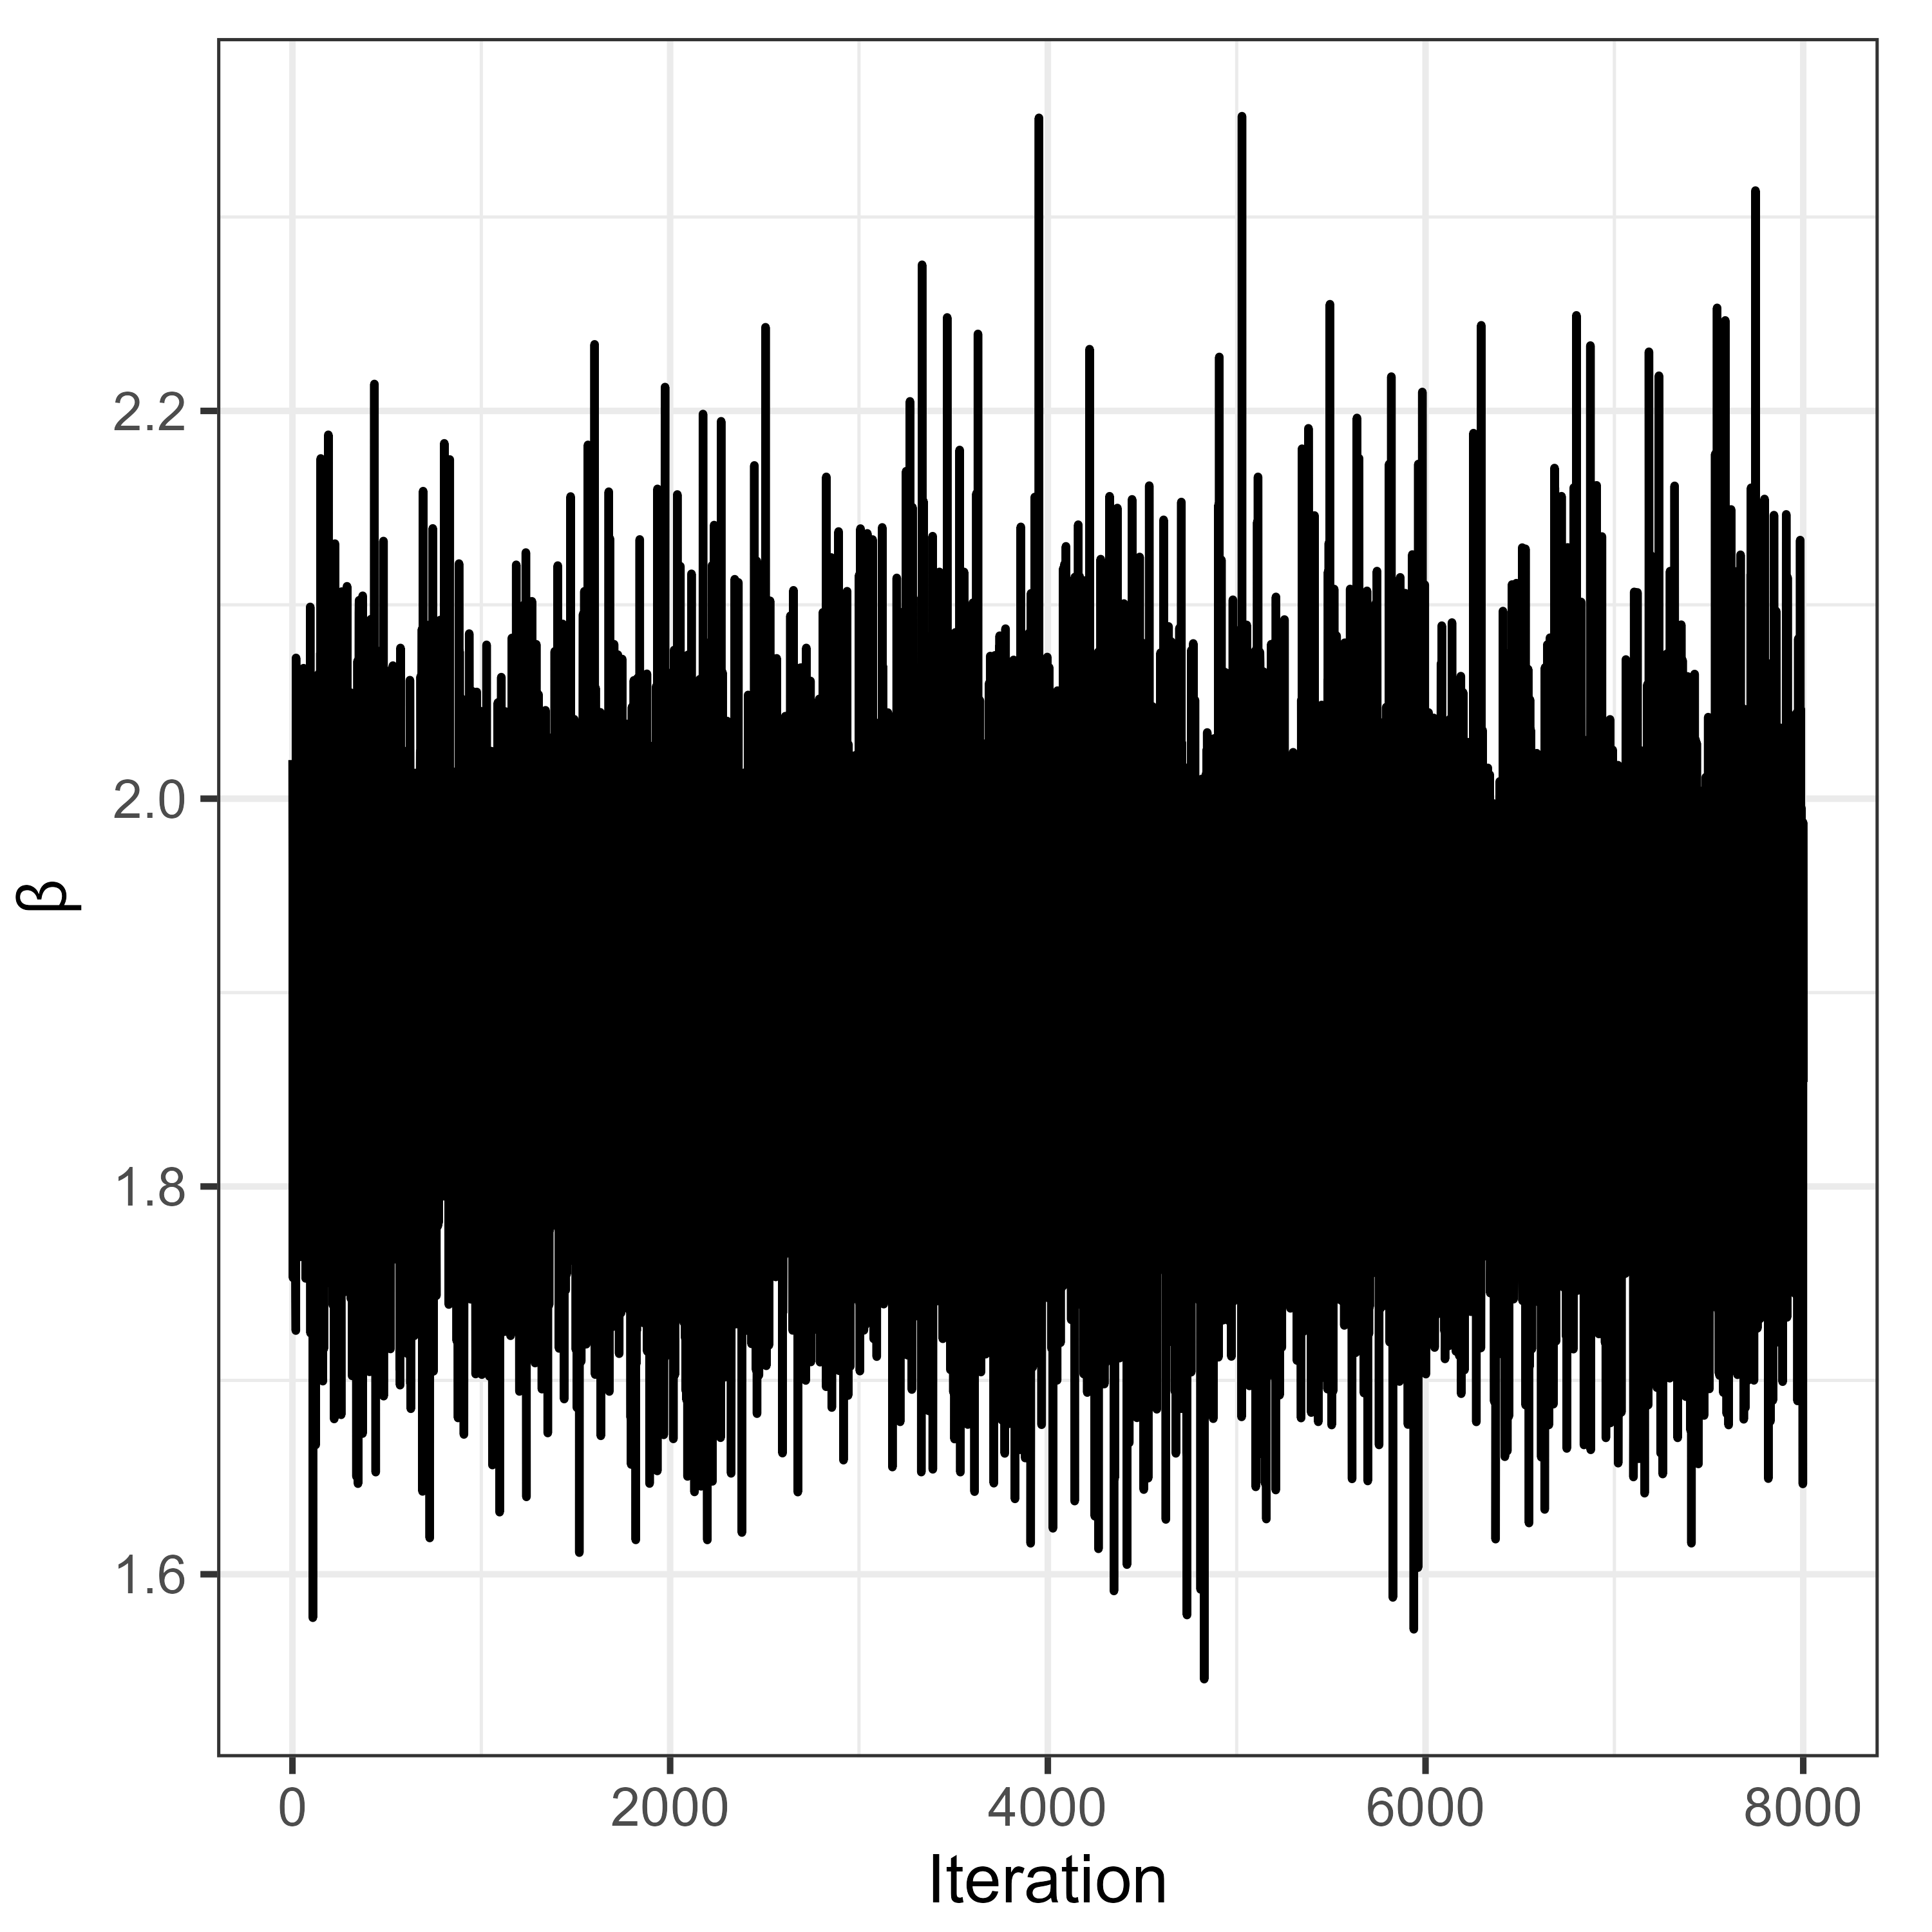
\includegraphics[width=0.6\textwidth]{../figures/simulation/trace_beta.png}
\caption{Traceplot of $\beta$ --- Simulation Study}
\label{fig:simulation_traceplot}
\end{figure}

The autocorrelation plot in Figure \ref{fig:simulation_autocorrelation} demonstrates low autocorrelation across lags, indicating good mixing of the Markov chain.

\begin{figure}[H]
\centering
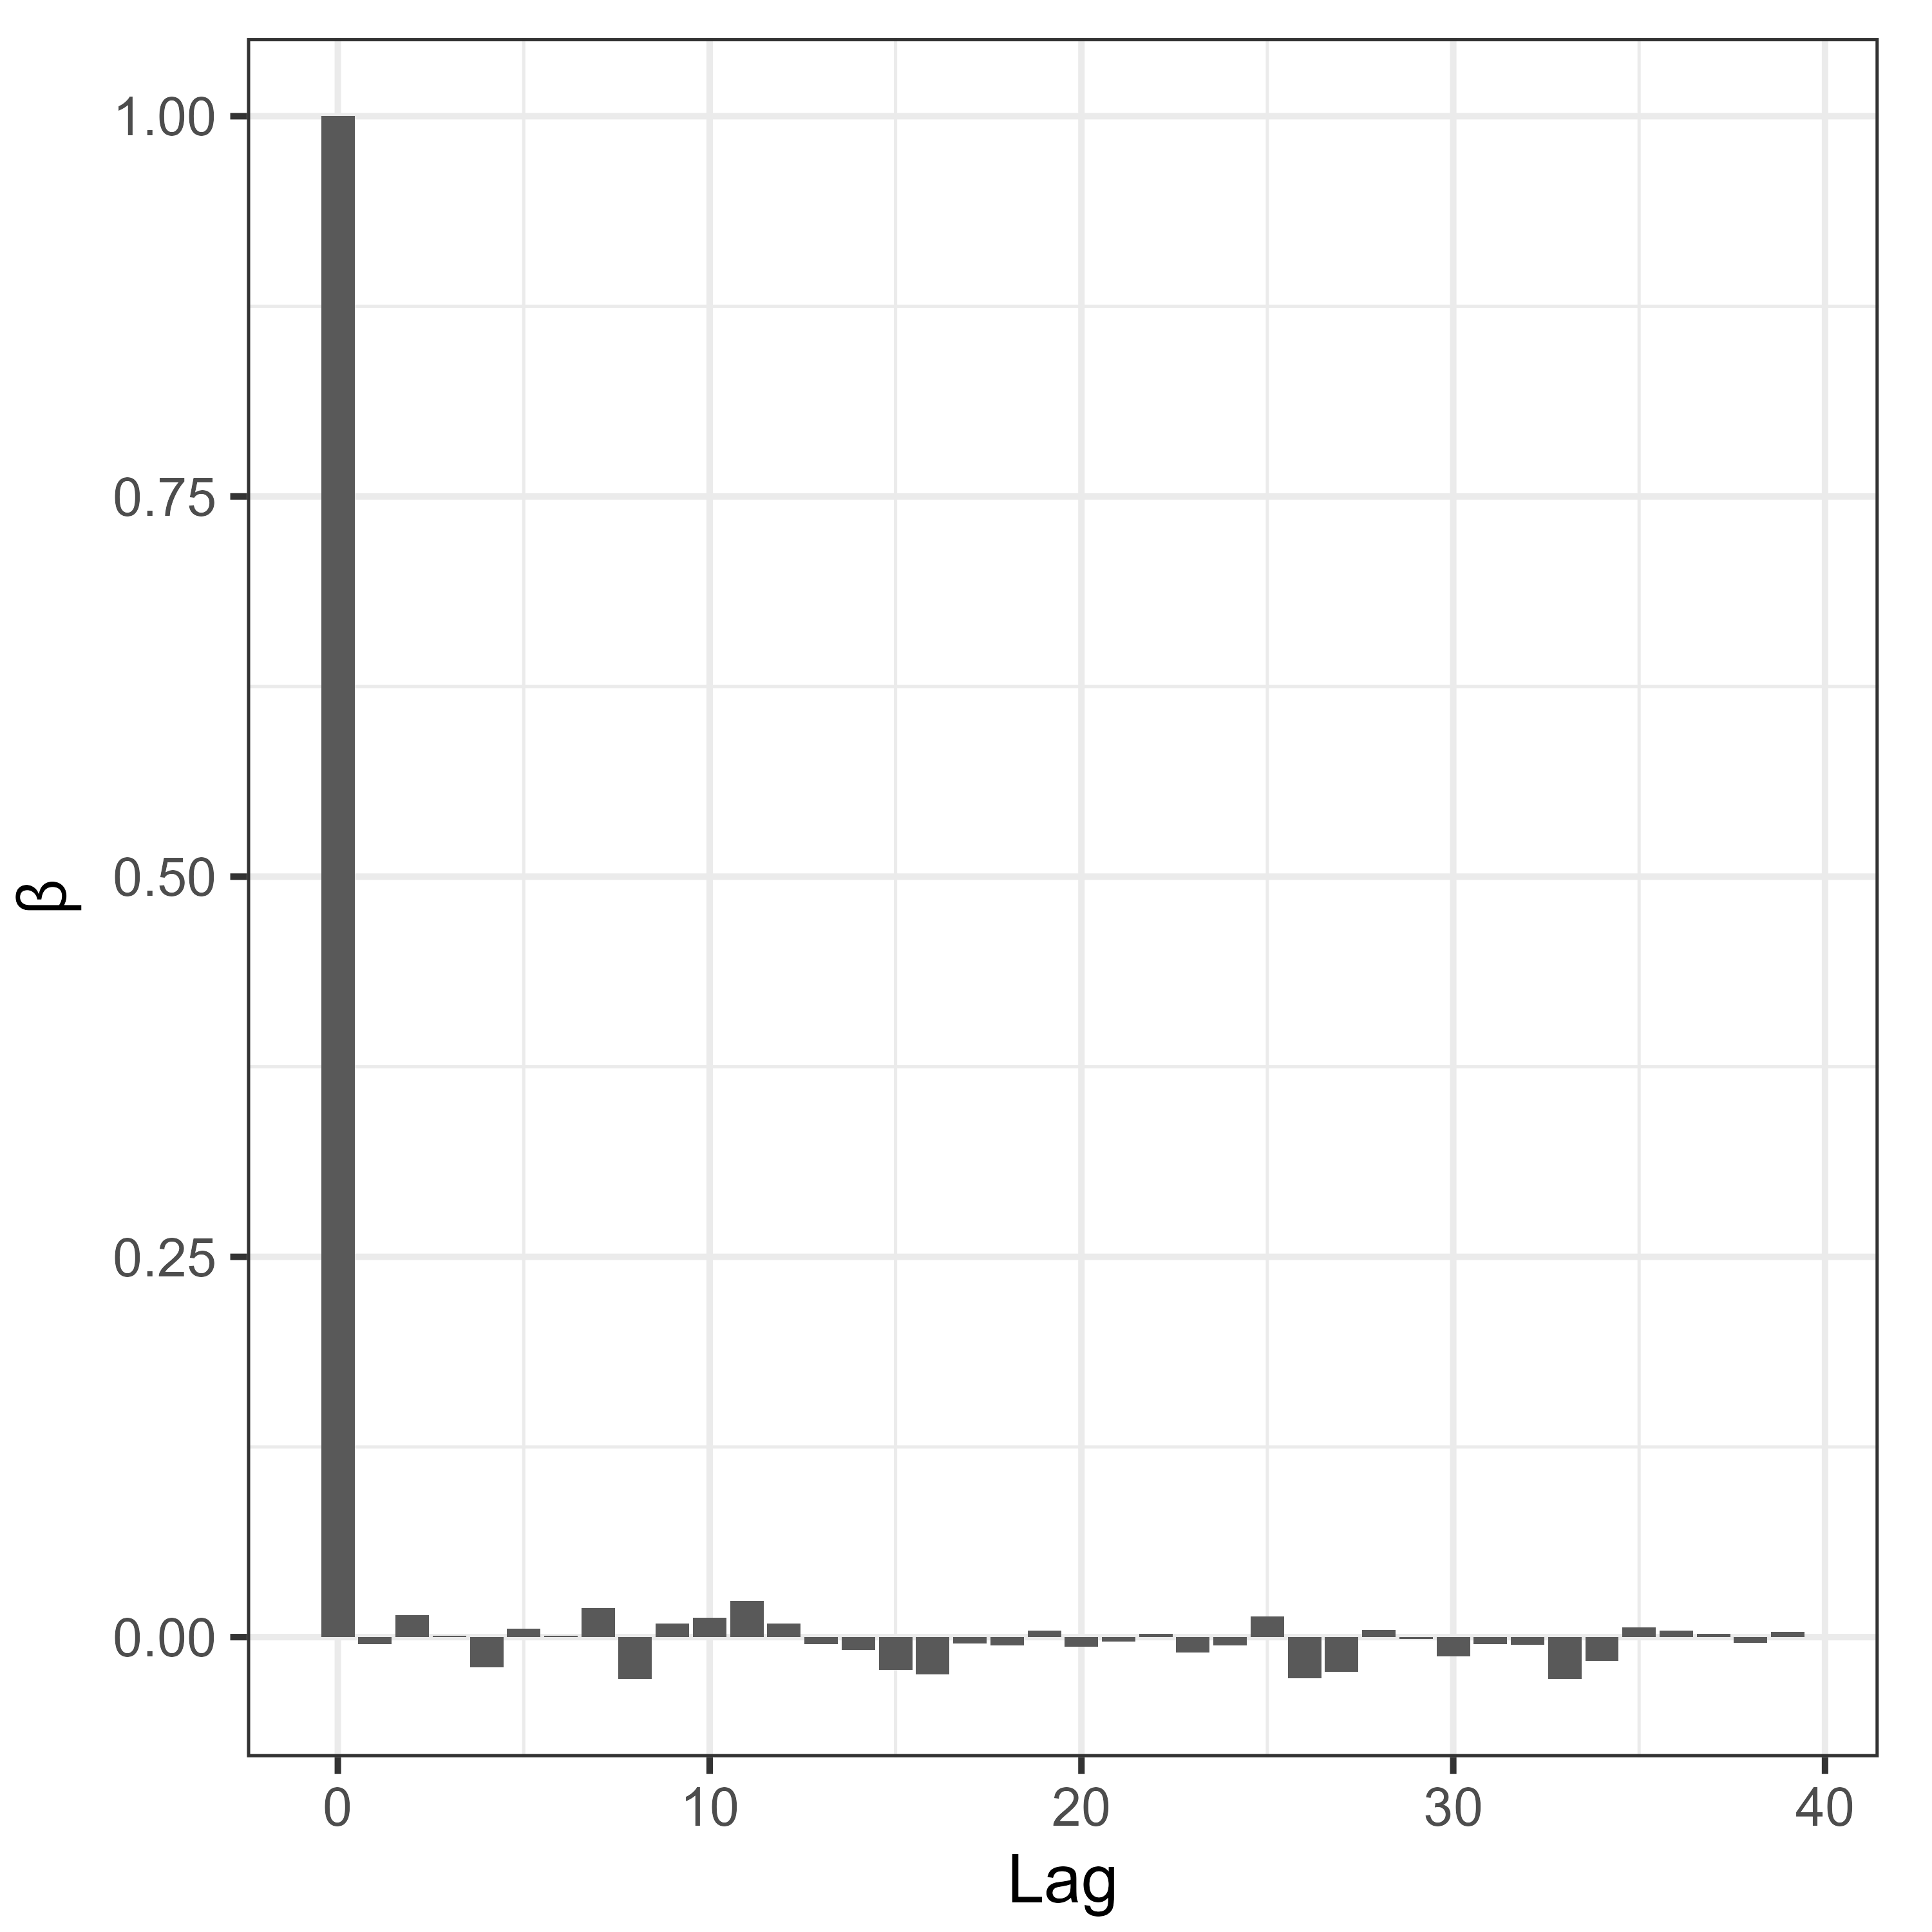
\includegraphics[width=0.6\textwidth]{../figures/simulation/acf_beta.png}
\caption{Autocorrelation of $\beta$ --- Simulation Study}
\label{fig:simulation_autocorrelation}
\end{figure}

We also plot the posterior distributions of the parameters in Figure \ref{fig:posterior_distributions} through histograms.

\begin{figure}[H]
\centering
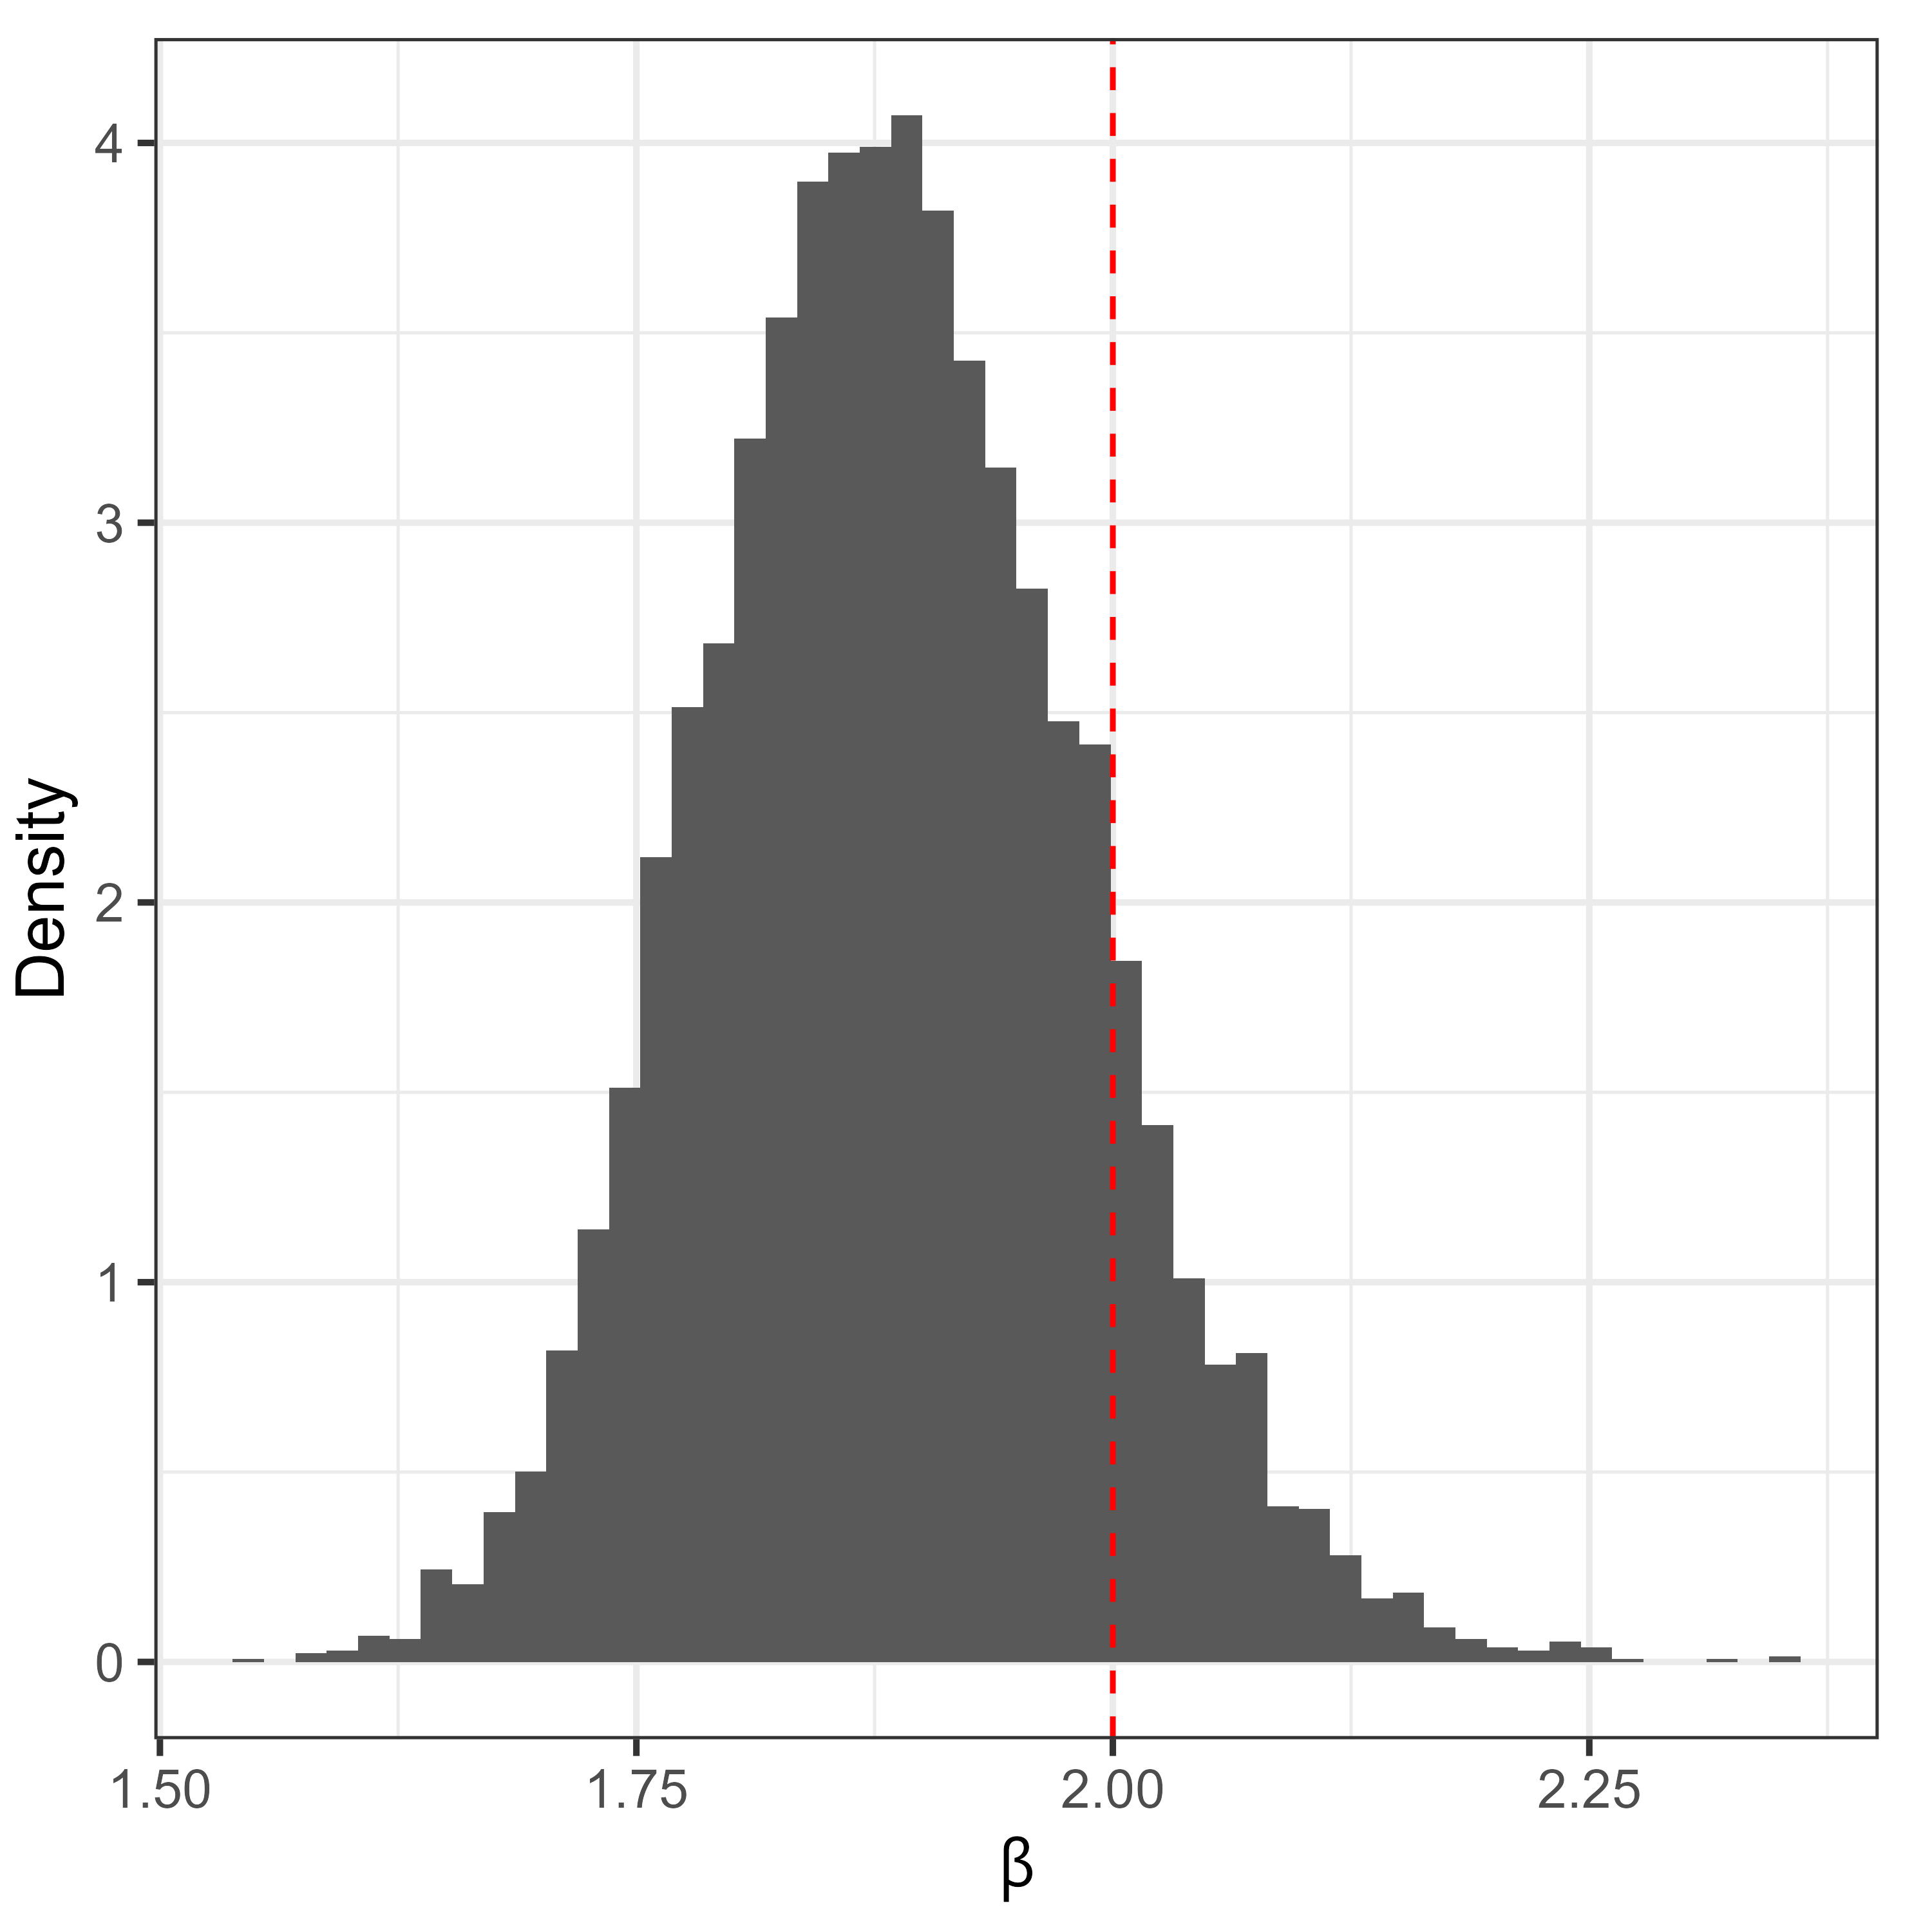
\includegraphics[width=0.6\textwidth]{../figures/simulation/hist_beta.png}
\caption{Posterior Distribution of $\beta$ --- Simulation Study}
\label{fig:posterior_distributions}
\end{figure}

As shown, the posterior distributions are centered close to the true parameter values, with minor deviations. This indicates that the Gibbs sampler successfully recovers the true parameters of the model under the simulated setting. As our sample size is relatively small, we would not expect to see a perfect recovery of the true parameters, but we cannot differentiate between the true and the estimated parameters. 

The other parameters also have a satisfactory recovery, as shown in Table \ref{tab:simulation_results} and the following figures. 

\begin{figure}[H]
    \centering
    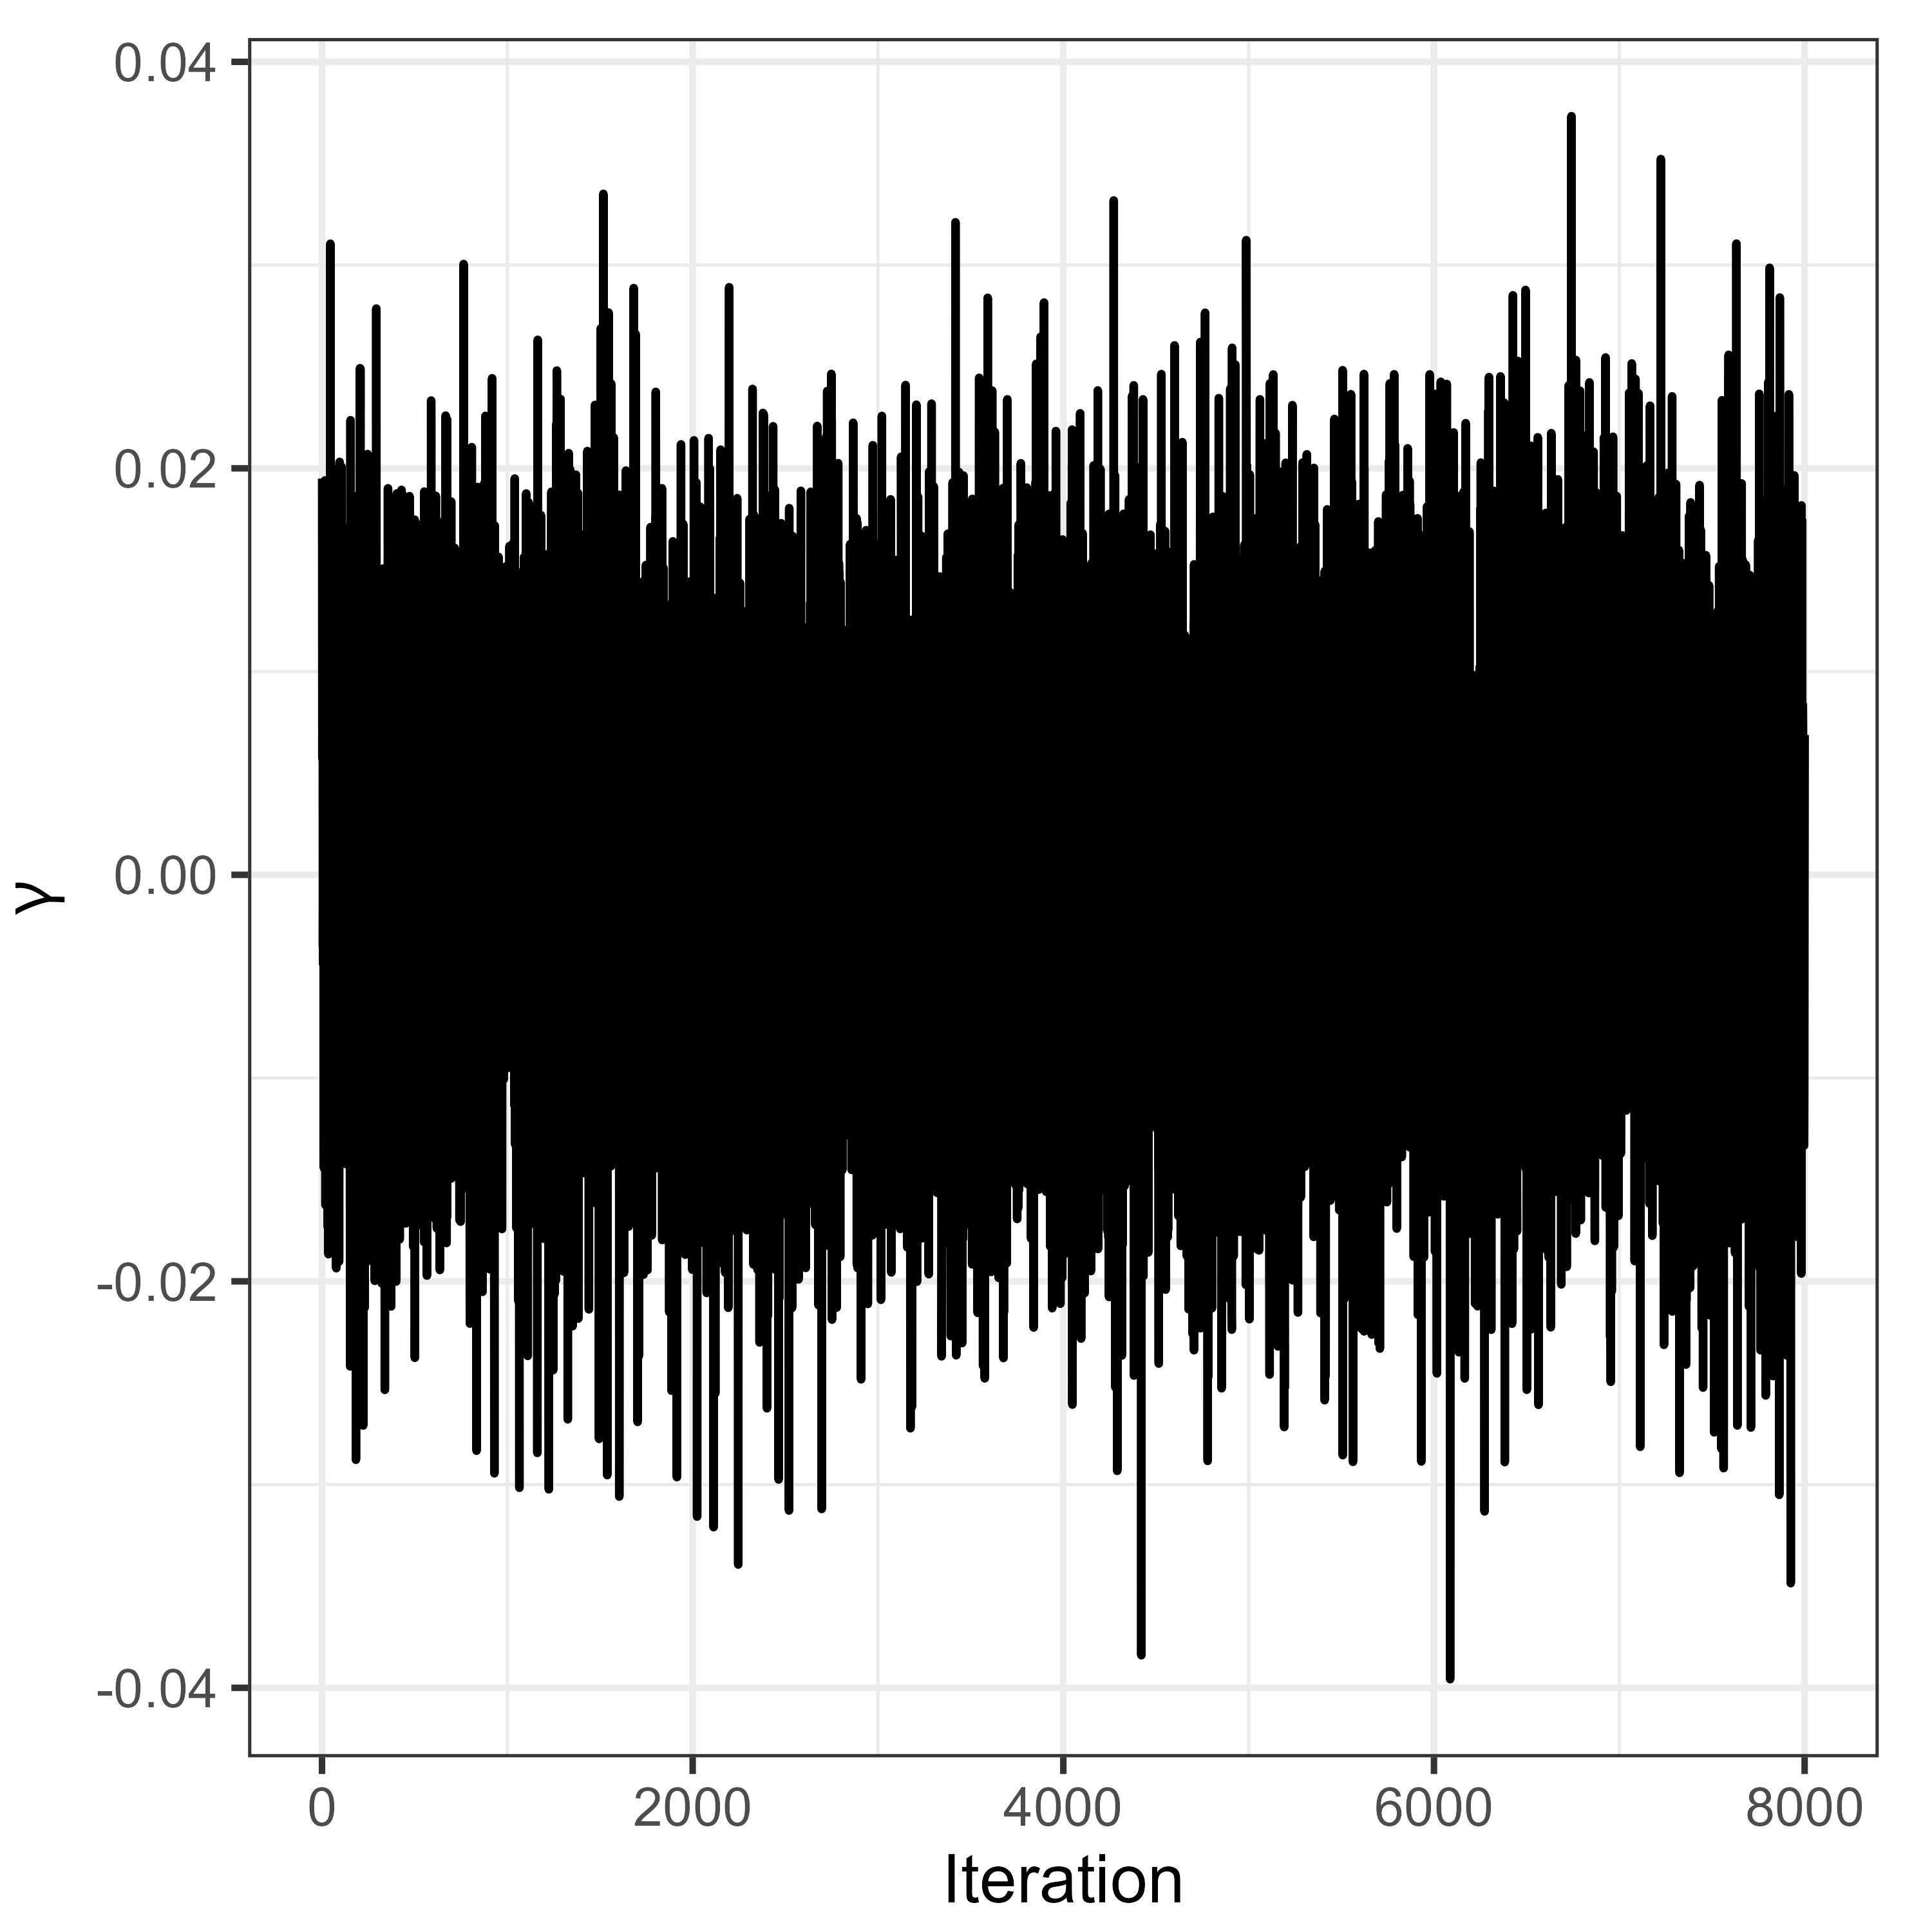
\includegraphics[width=0.45\textwidth]{../figures/simulation/trace_gamma.png}
    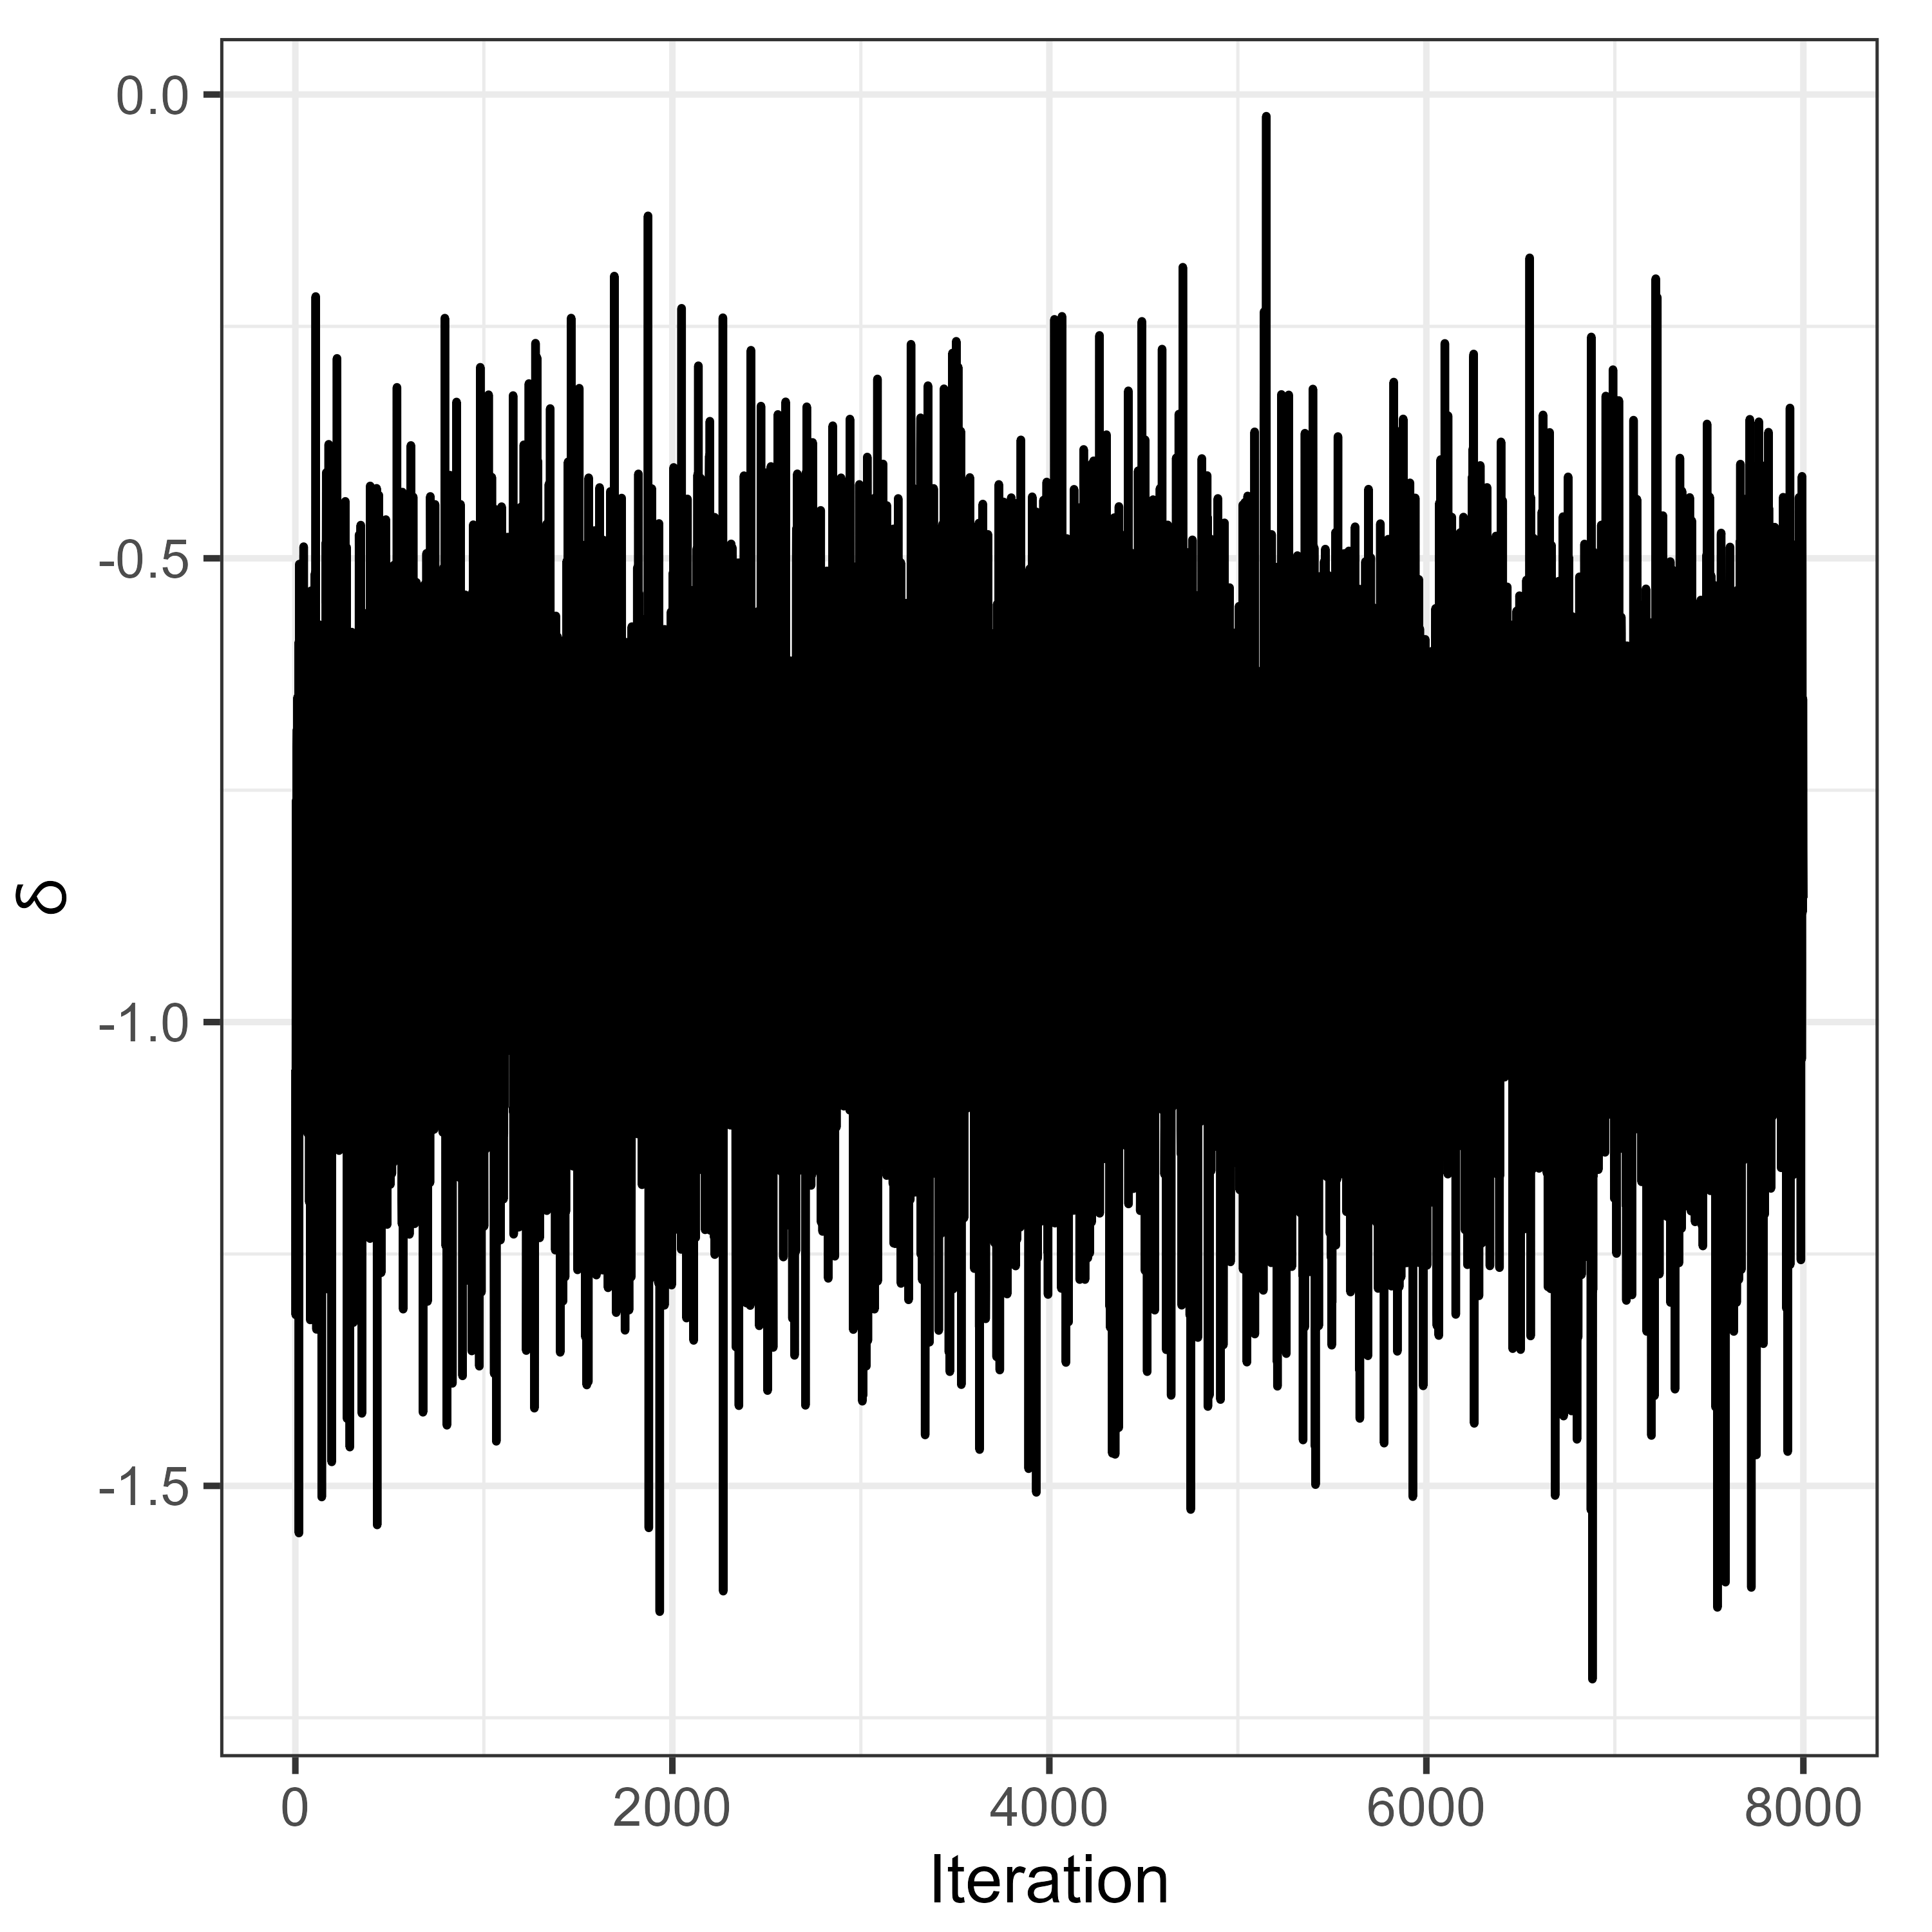
\includegraphics[width=0.45\textwidth]{../figures/simulation/trace_delta.png}
    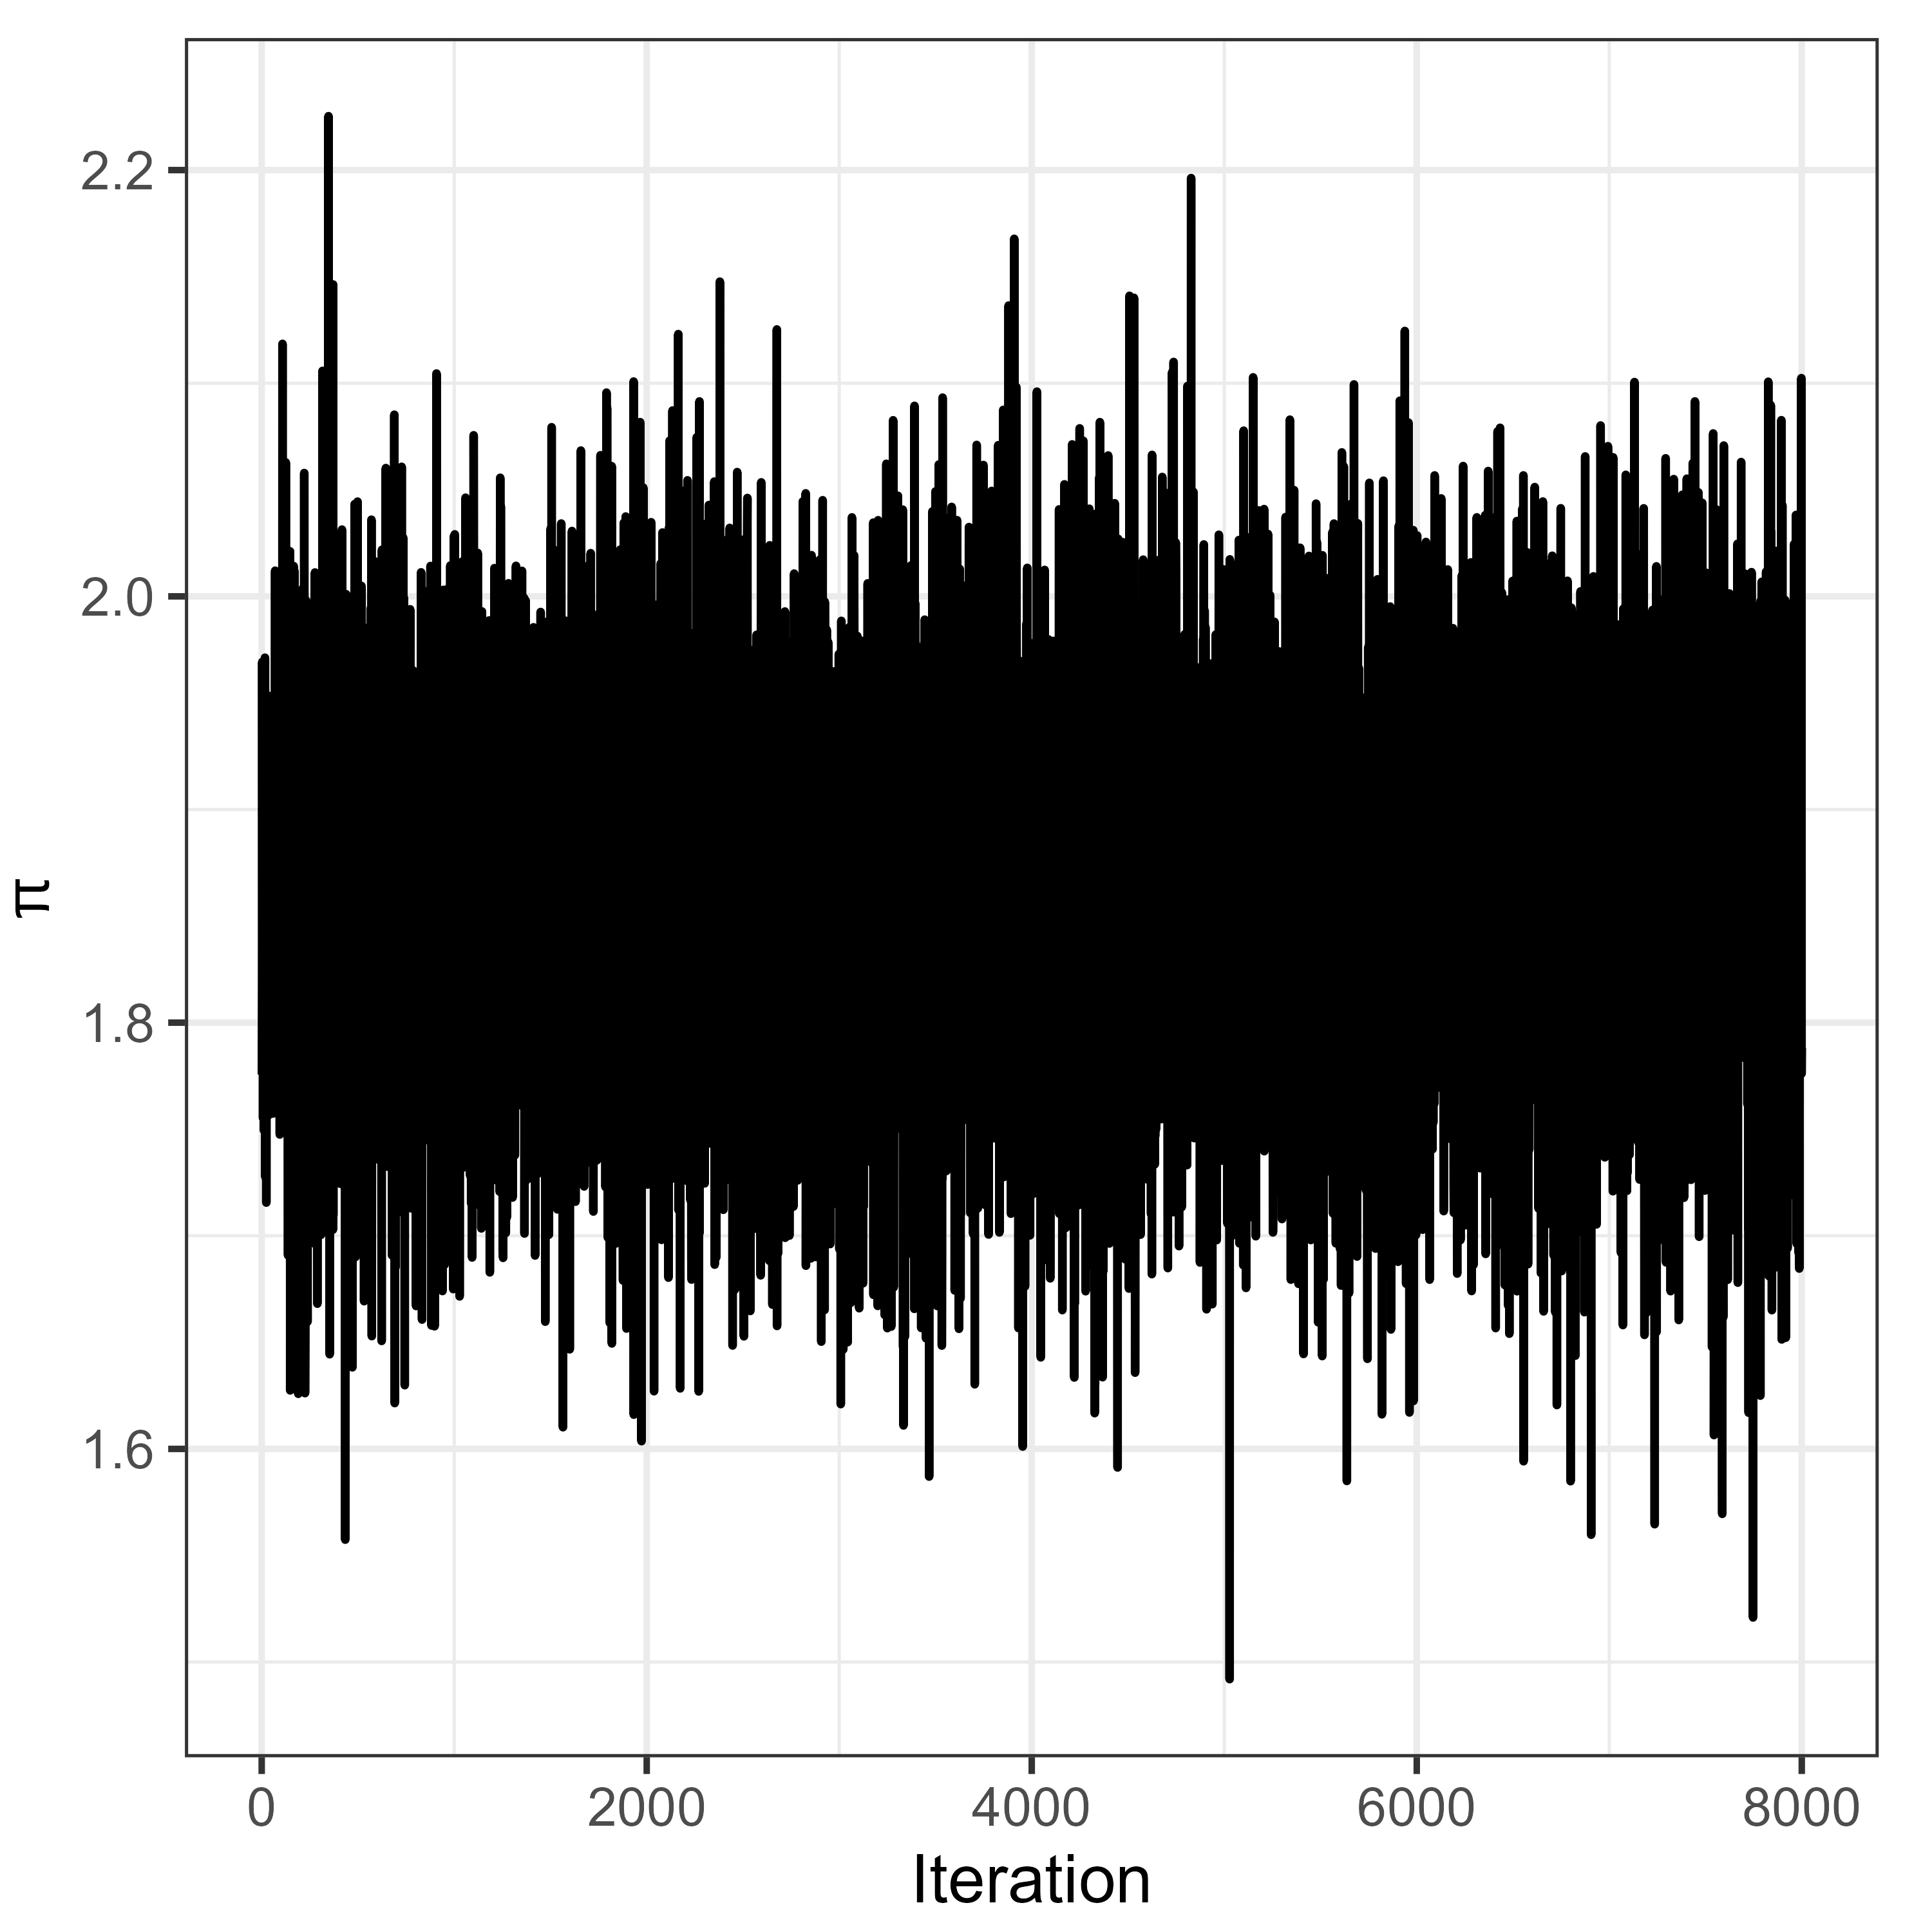
\includegraphics[width=0.45\textwidth]{../figures/simulation/trace_pi.png}
    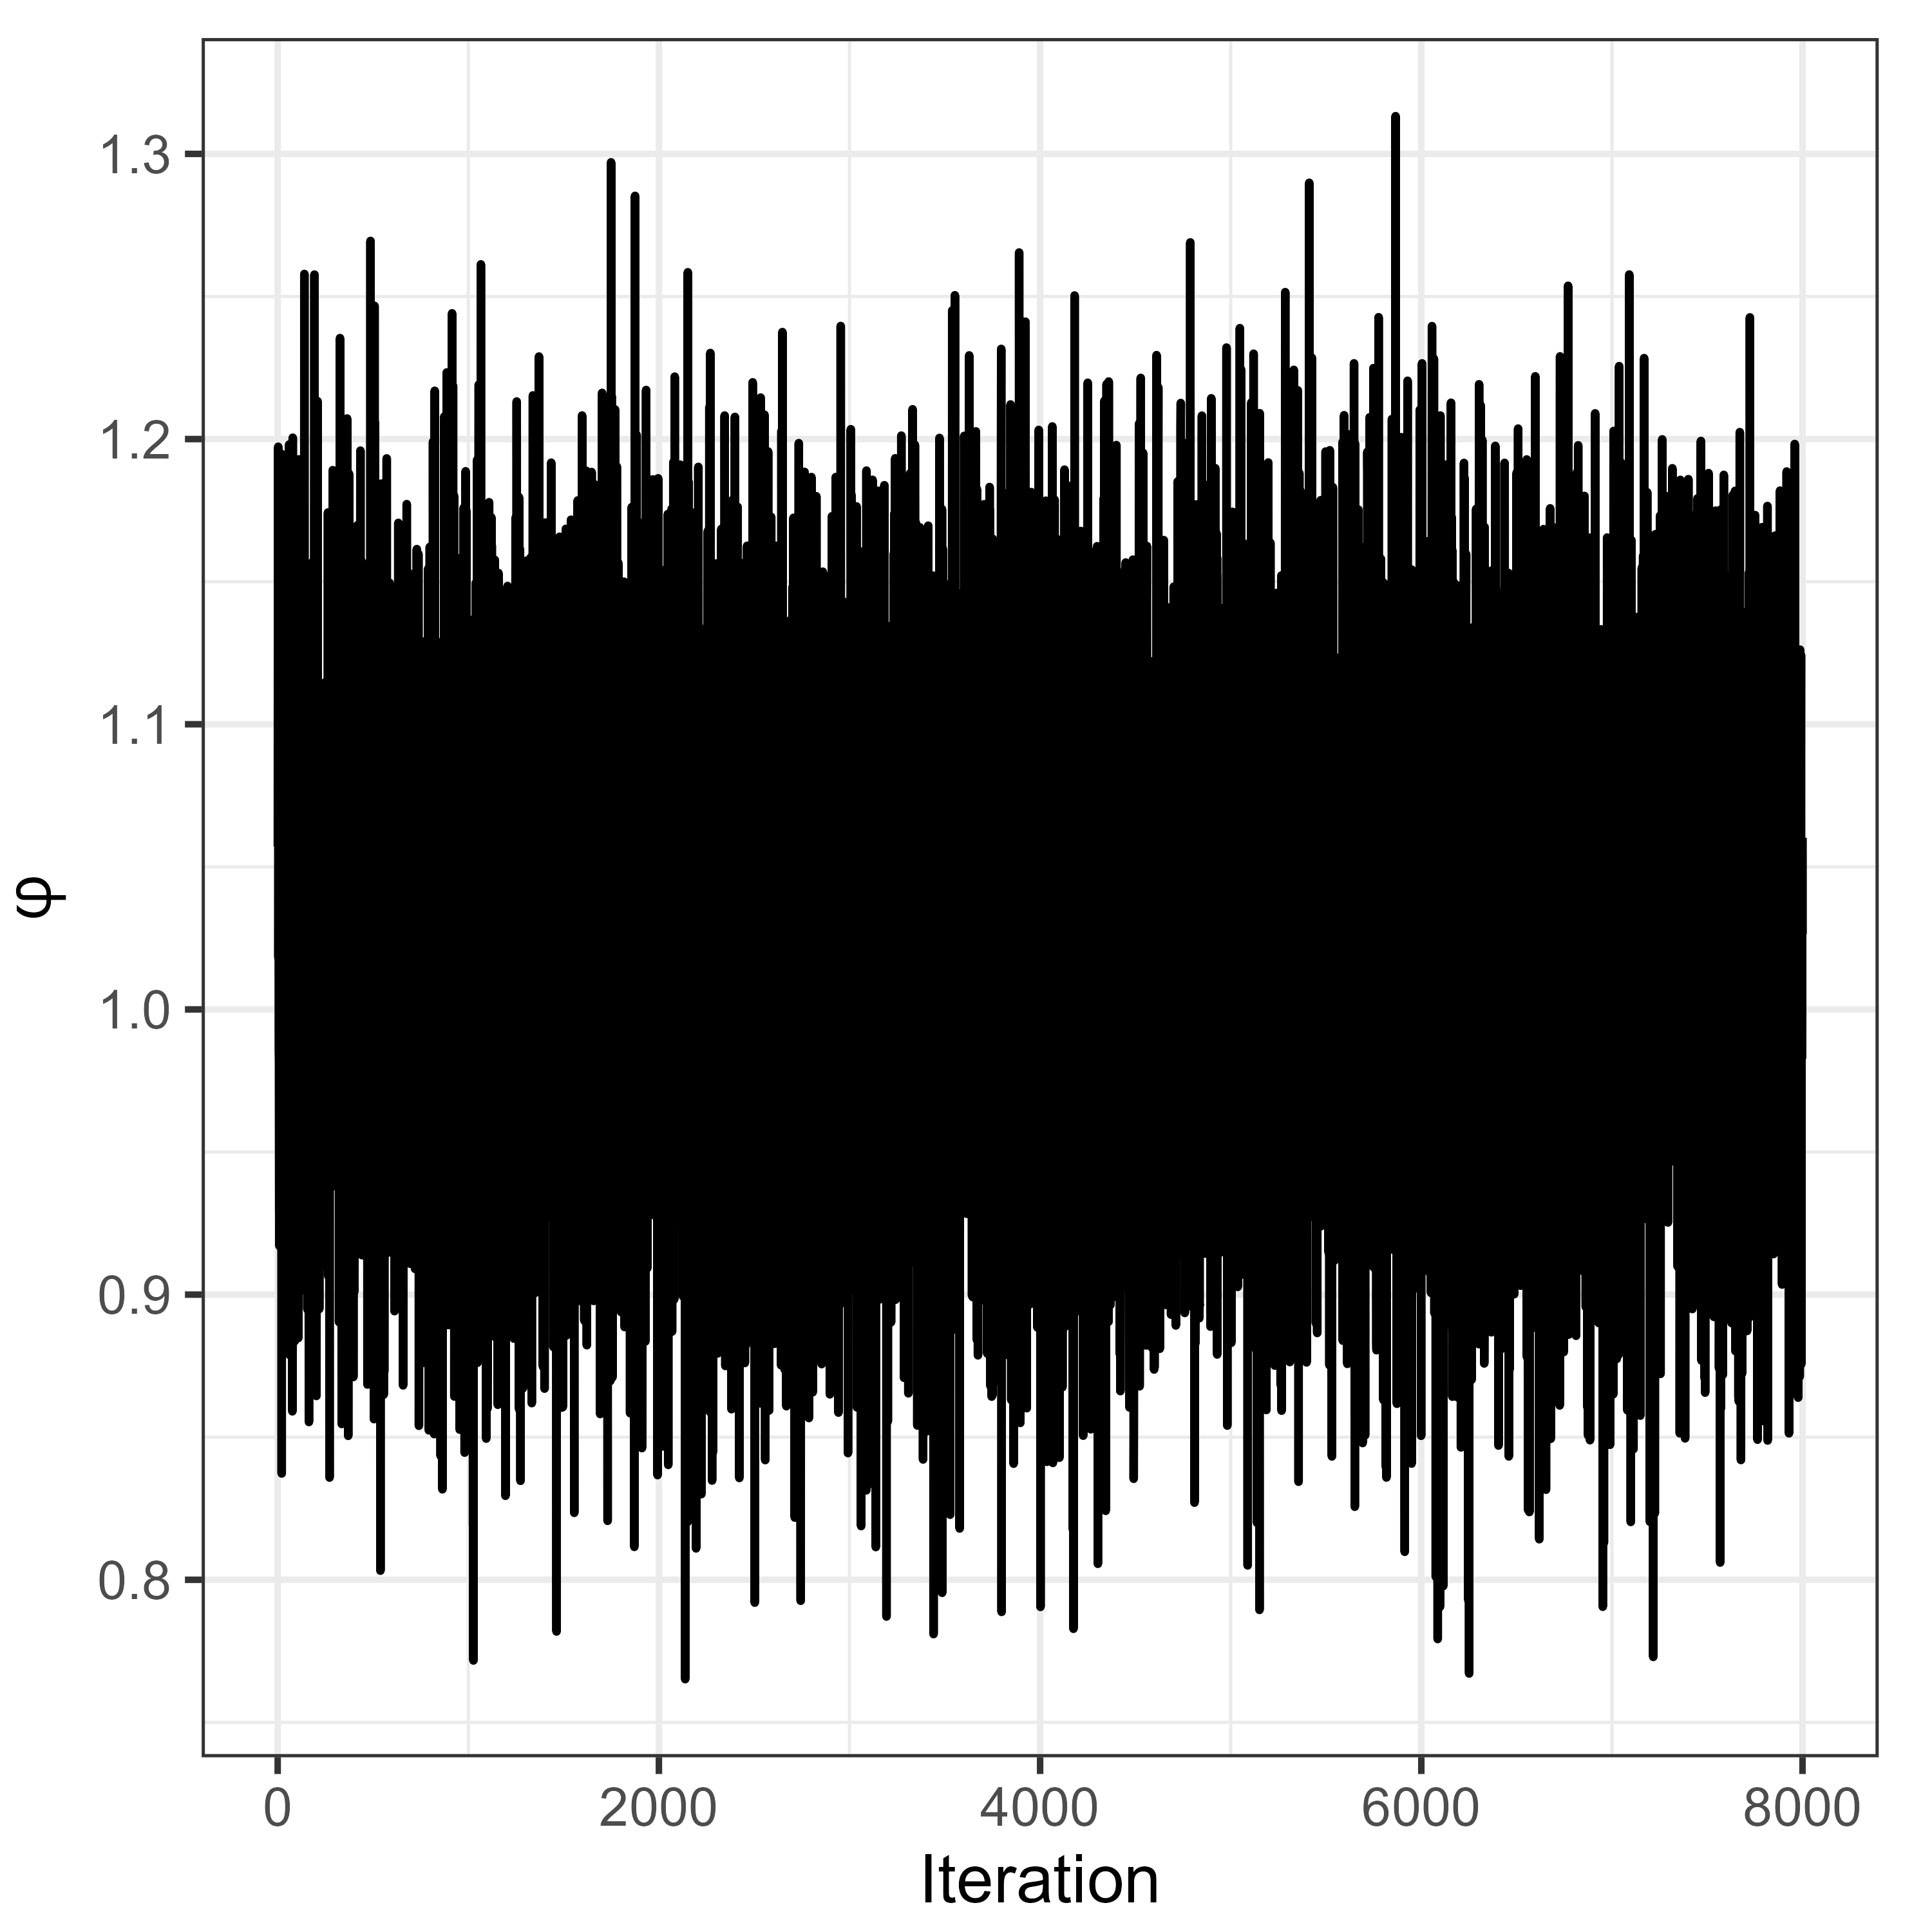
\includegraphics[width=0.45\textwidth]{../figures/simulation/trace_phi.png}
    \caption{Traceplots of $\gamma$, $\delta$, $\pi$, and $\phi$ --- Simulation Study}
    \label{fig:posterior_traceplots_2}
    \end{figure}
    
\begin{figure}[H]
    \centering
    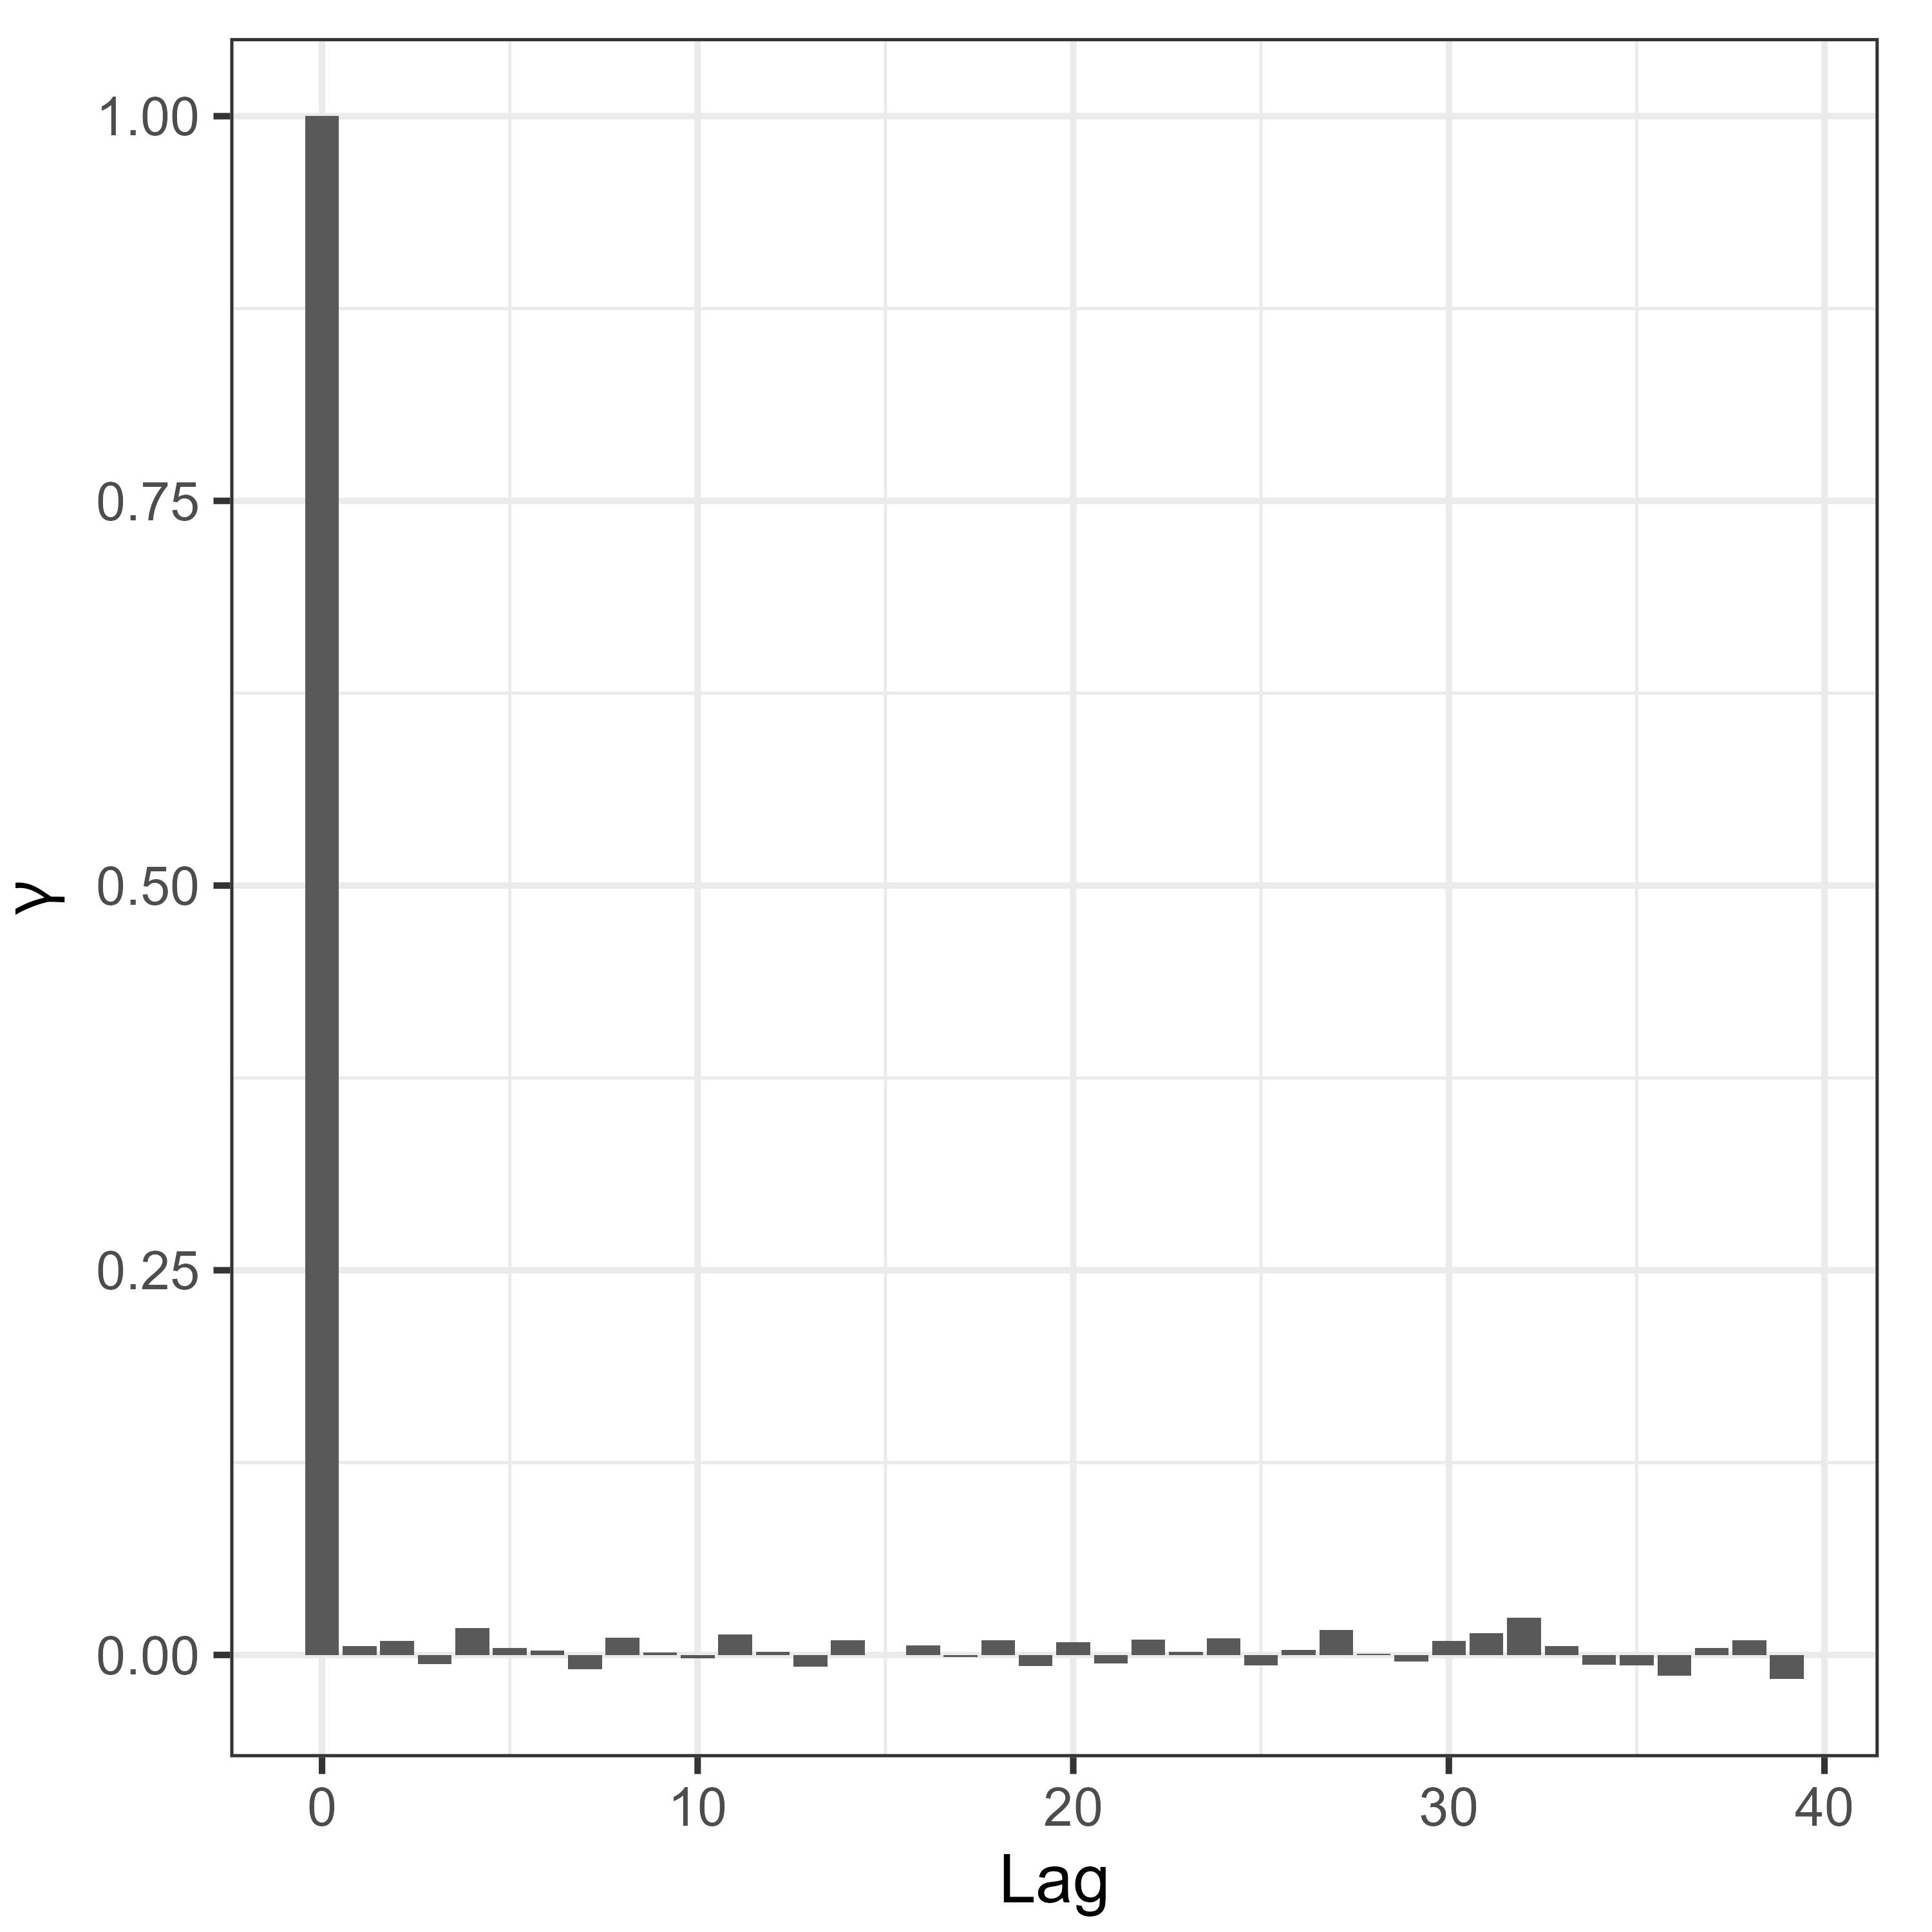
\includegraphics[width=0.45\textwidth]{../figures/simulation/acf_gamma.png}
    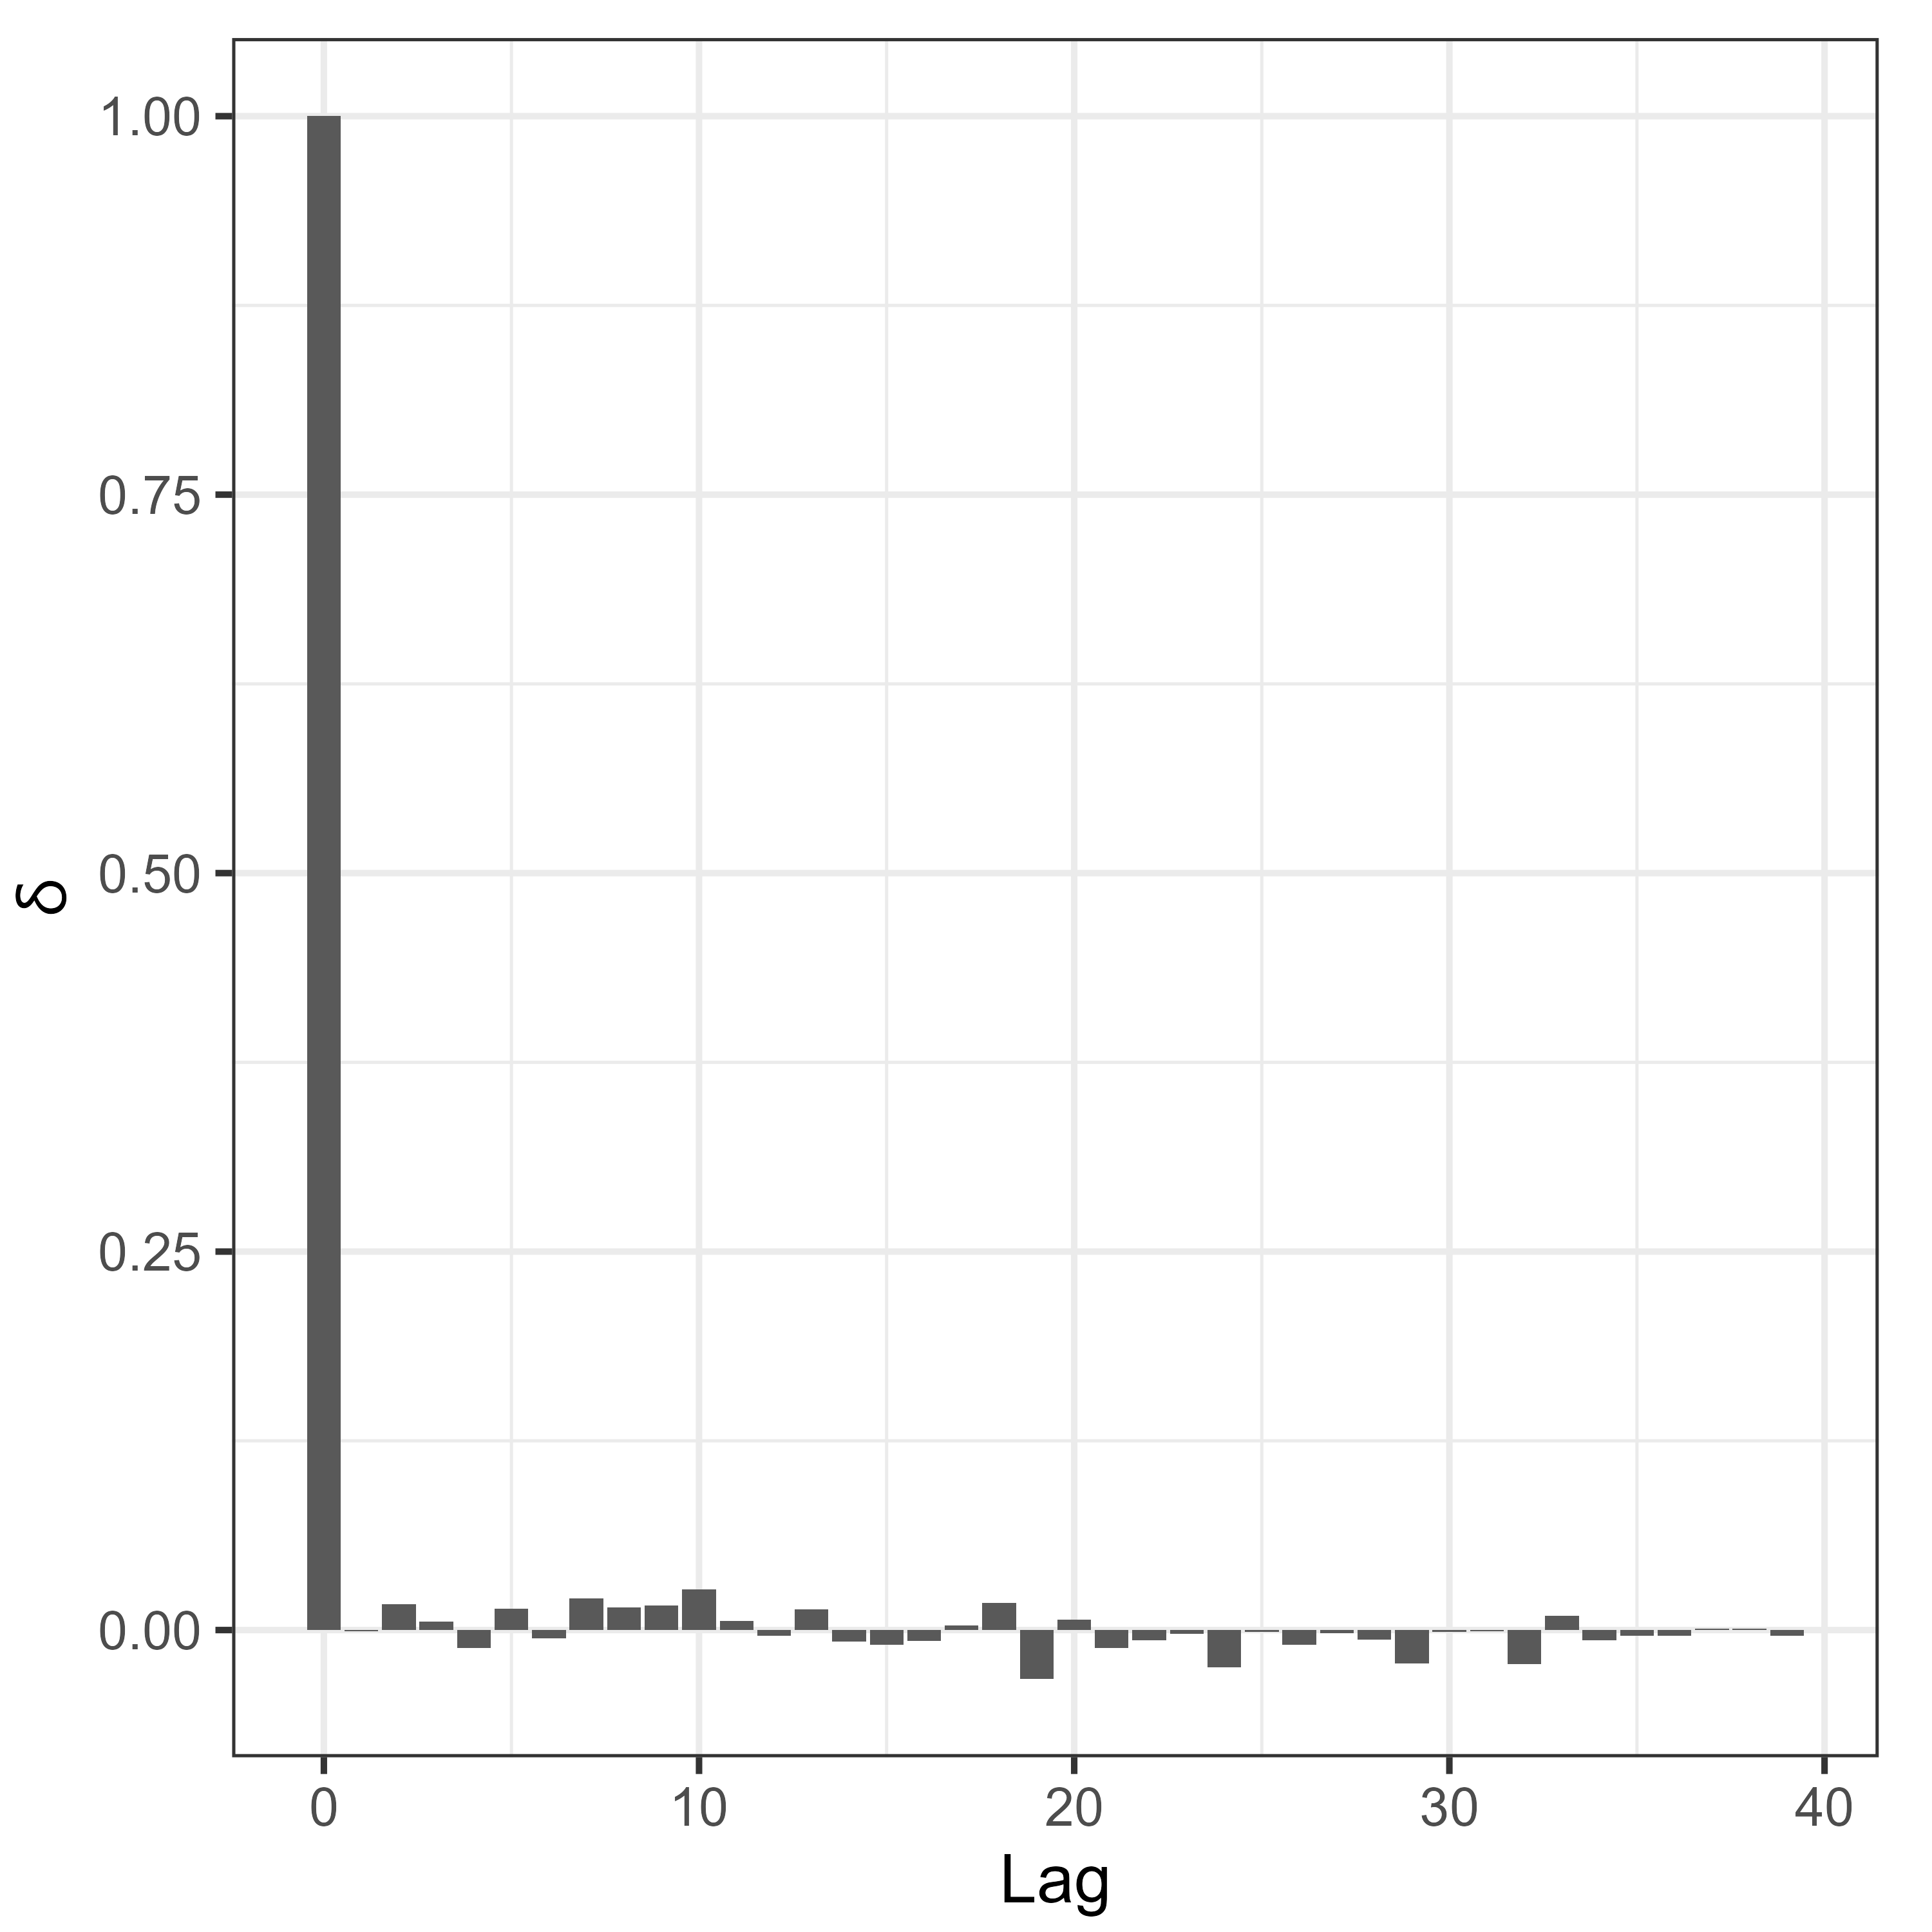
\includegraphics[width=0.45\textwidth]{../figures/simulation/acf_delta.png}
    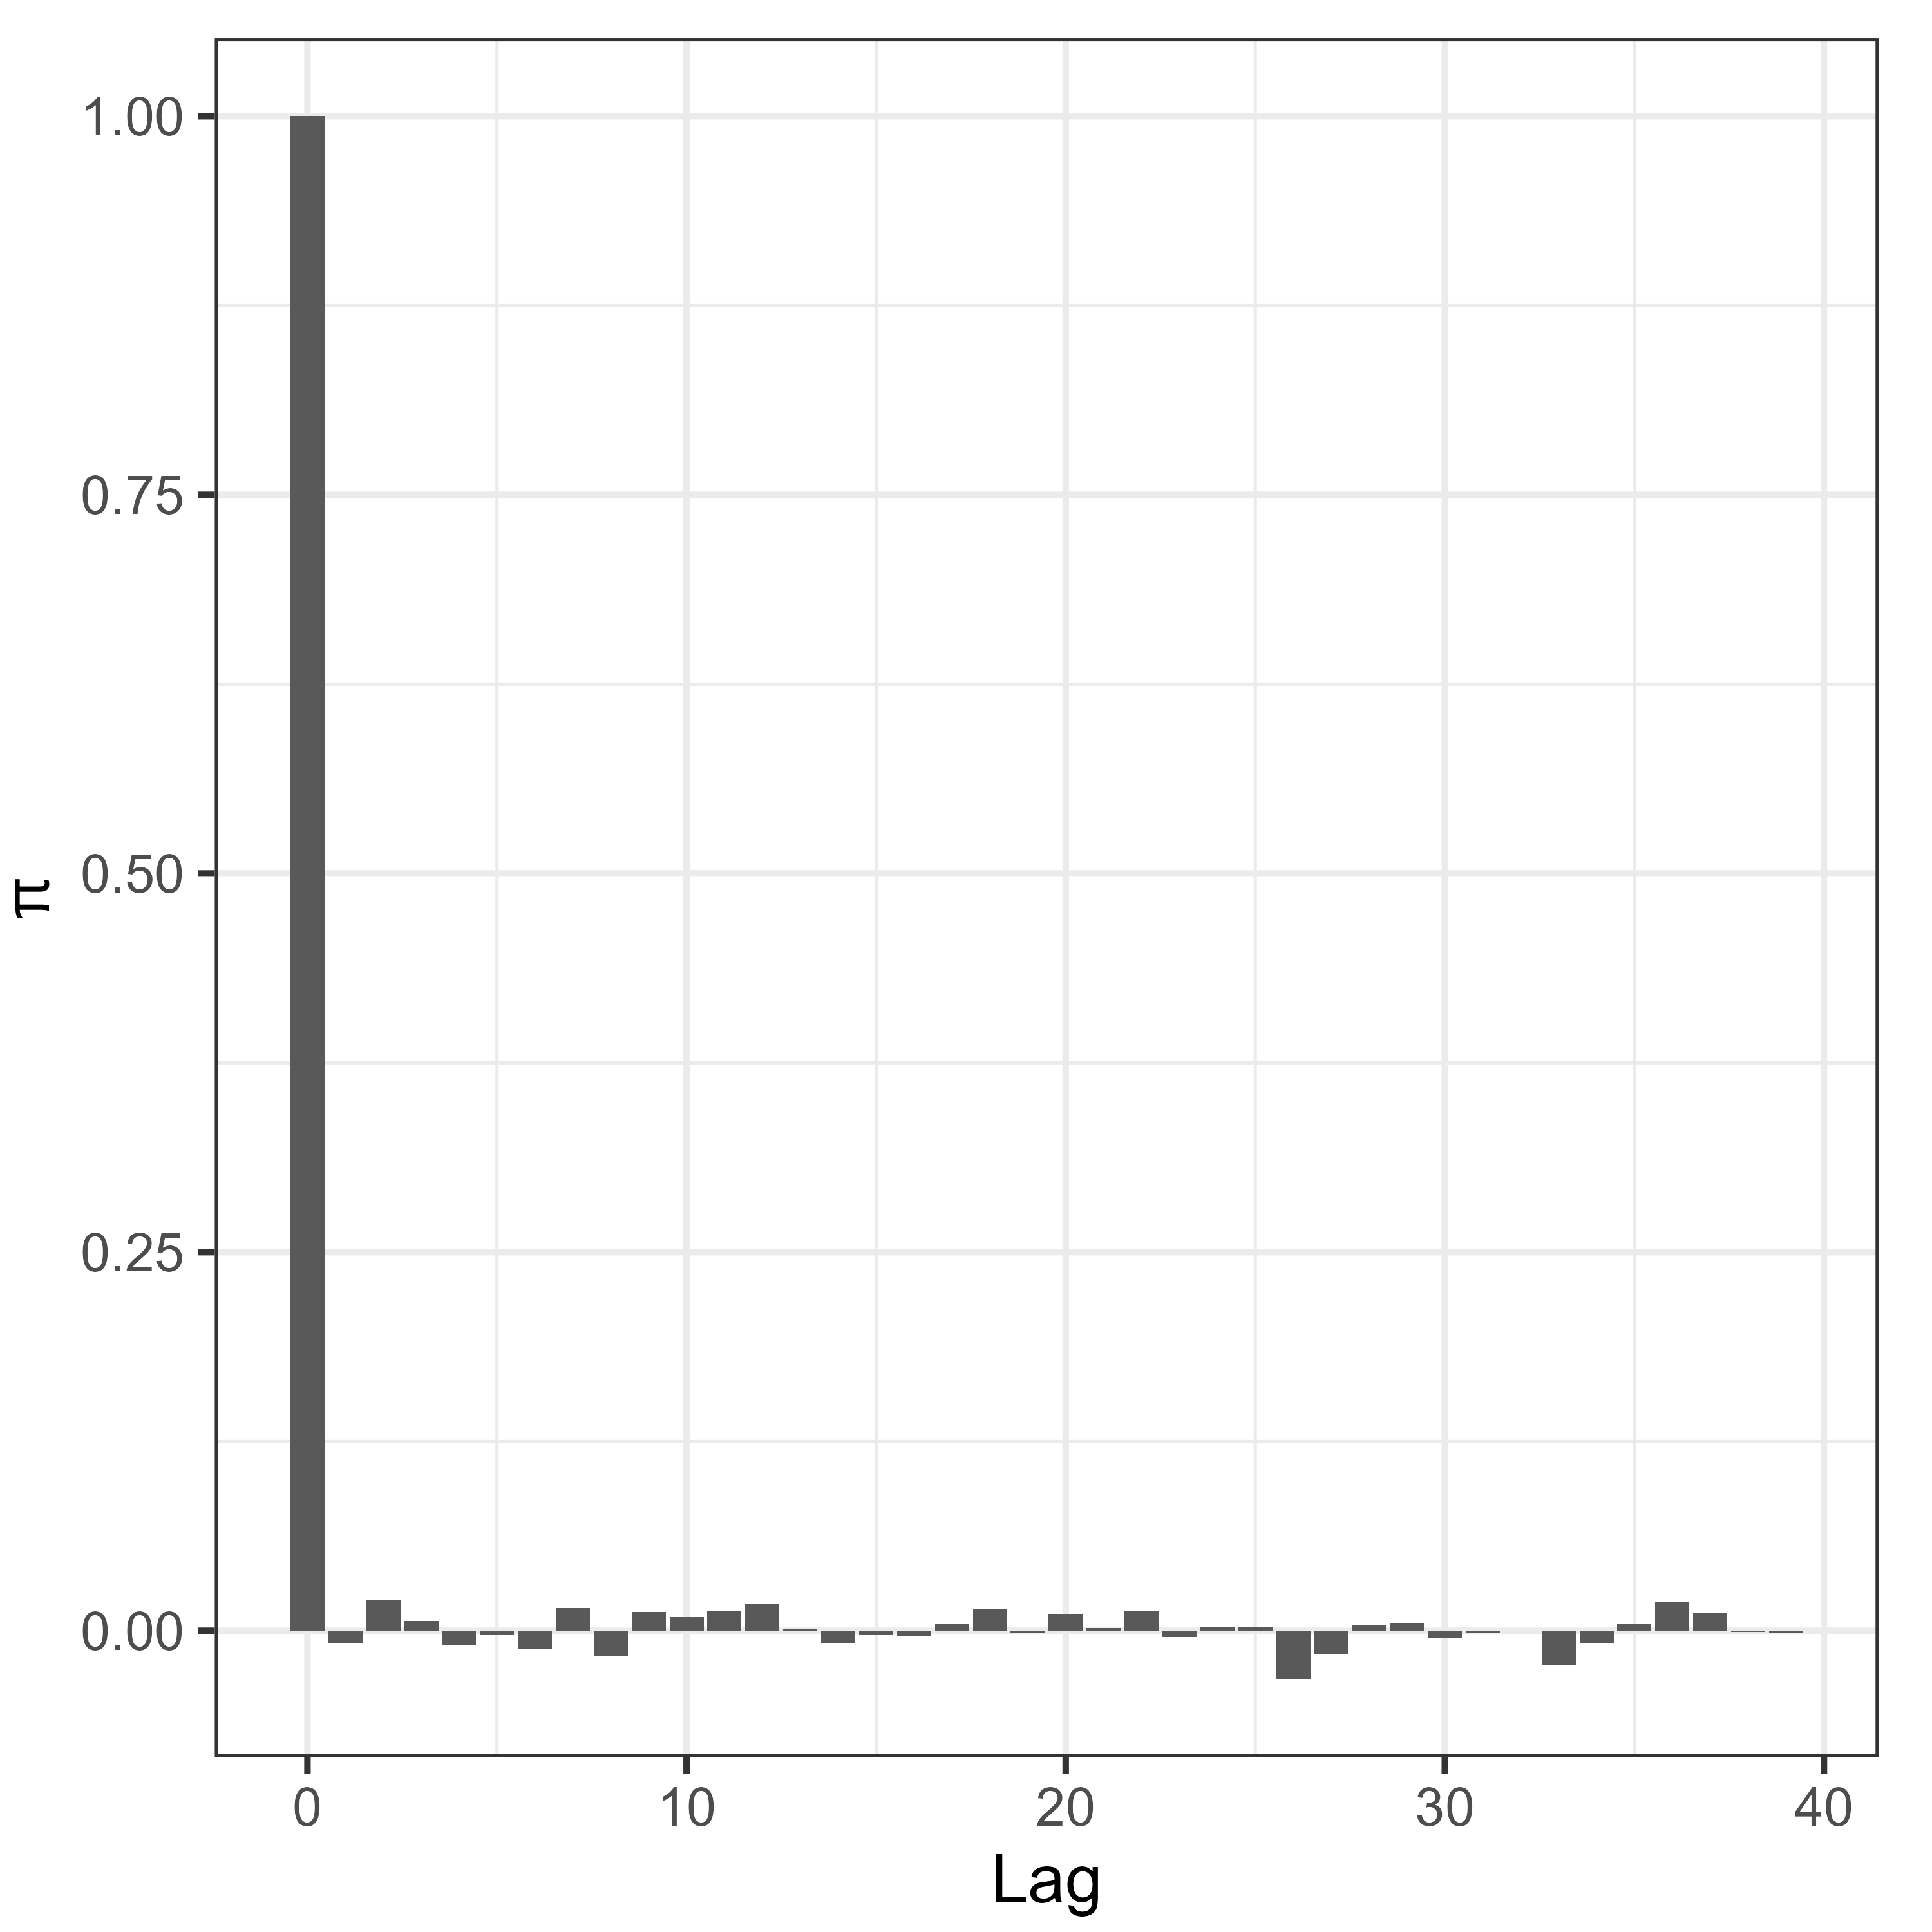
\includegraphics[width=0.45\textwidth]{../figures/simulation/acf_pi.png}
    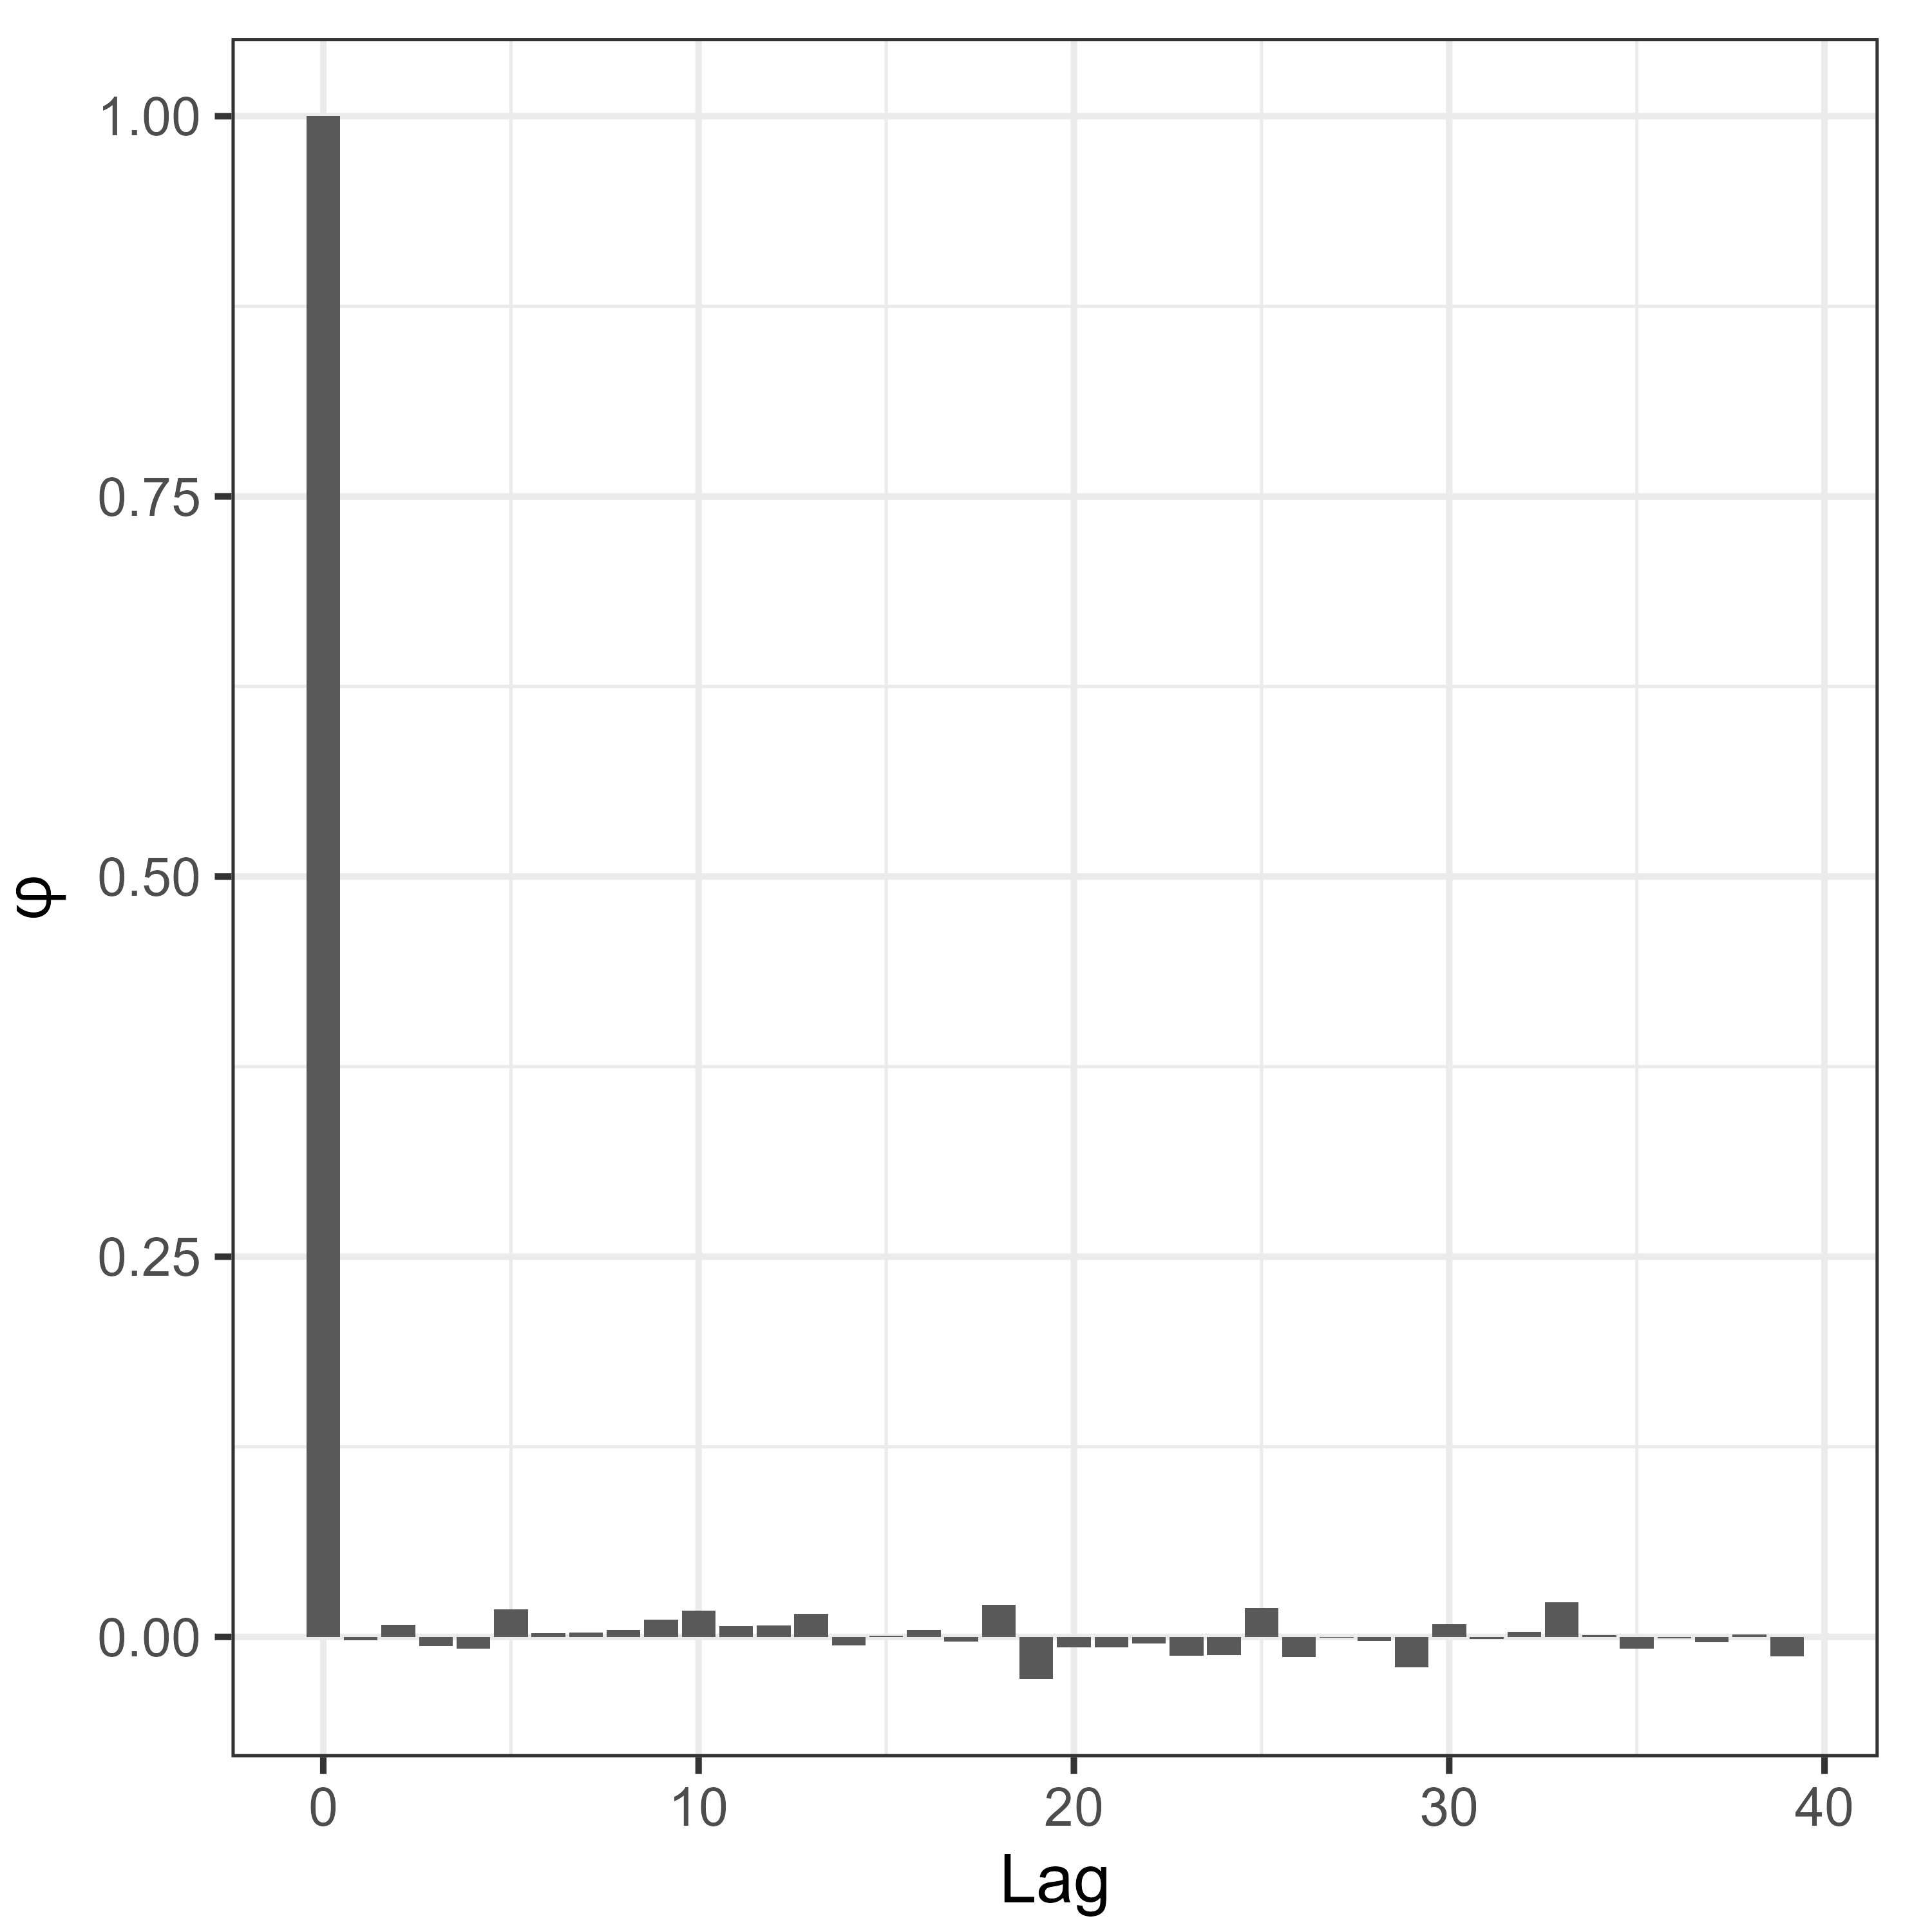
\includegraphics[width=0.45\textwidth]{../figures/simulation/acf_phi.png}
    \caption{Autocorrelation of $\gamma$, $\delta$, $\pi$, and $\phi$ --- Simulation Study}
    \label{fig:posterior_autocorrelation_2}
\end{figure}    
    
\begin{figure}[H]
\centering
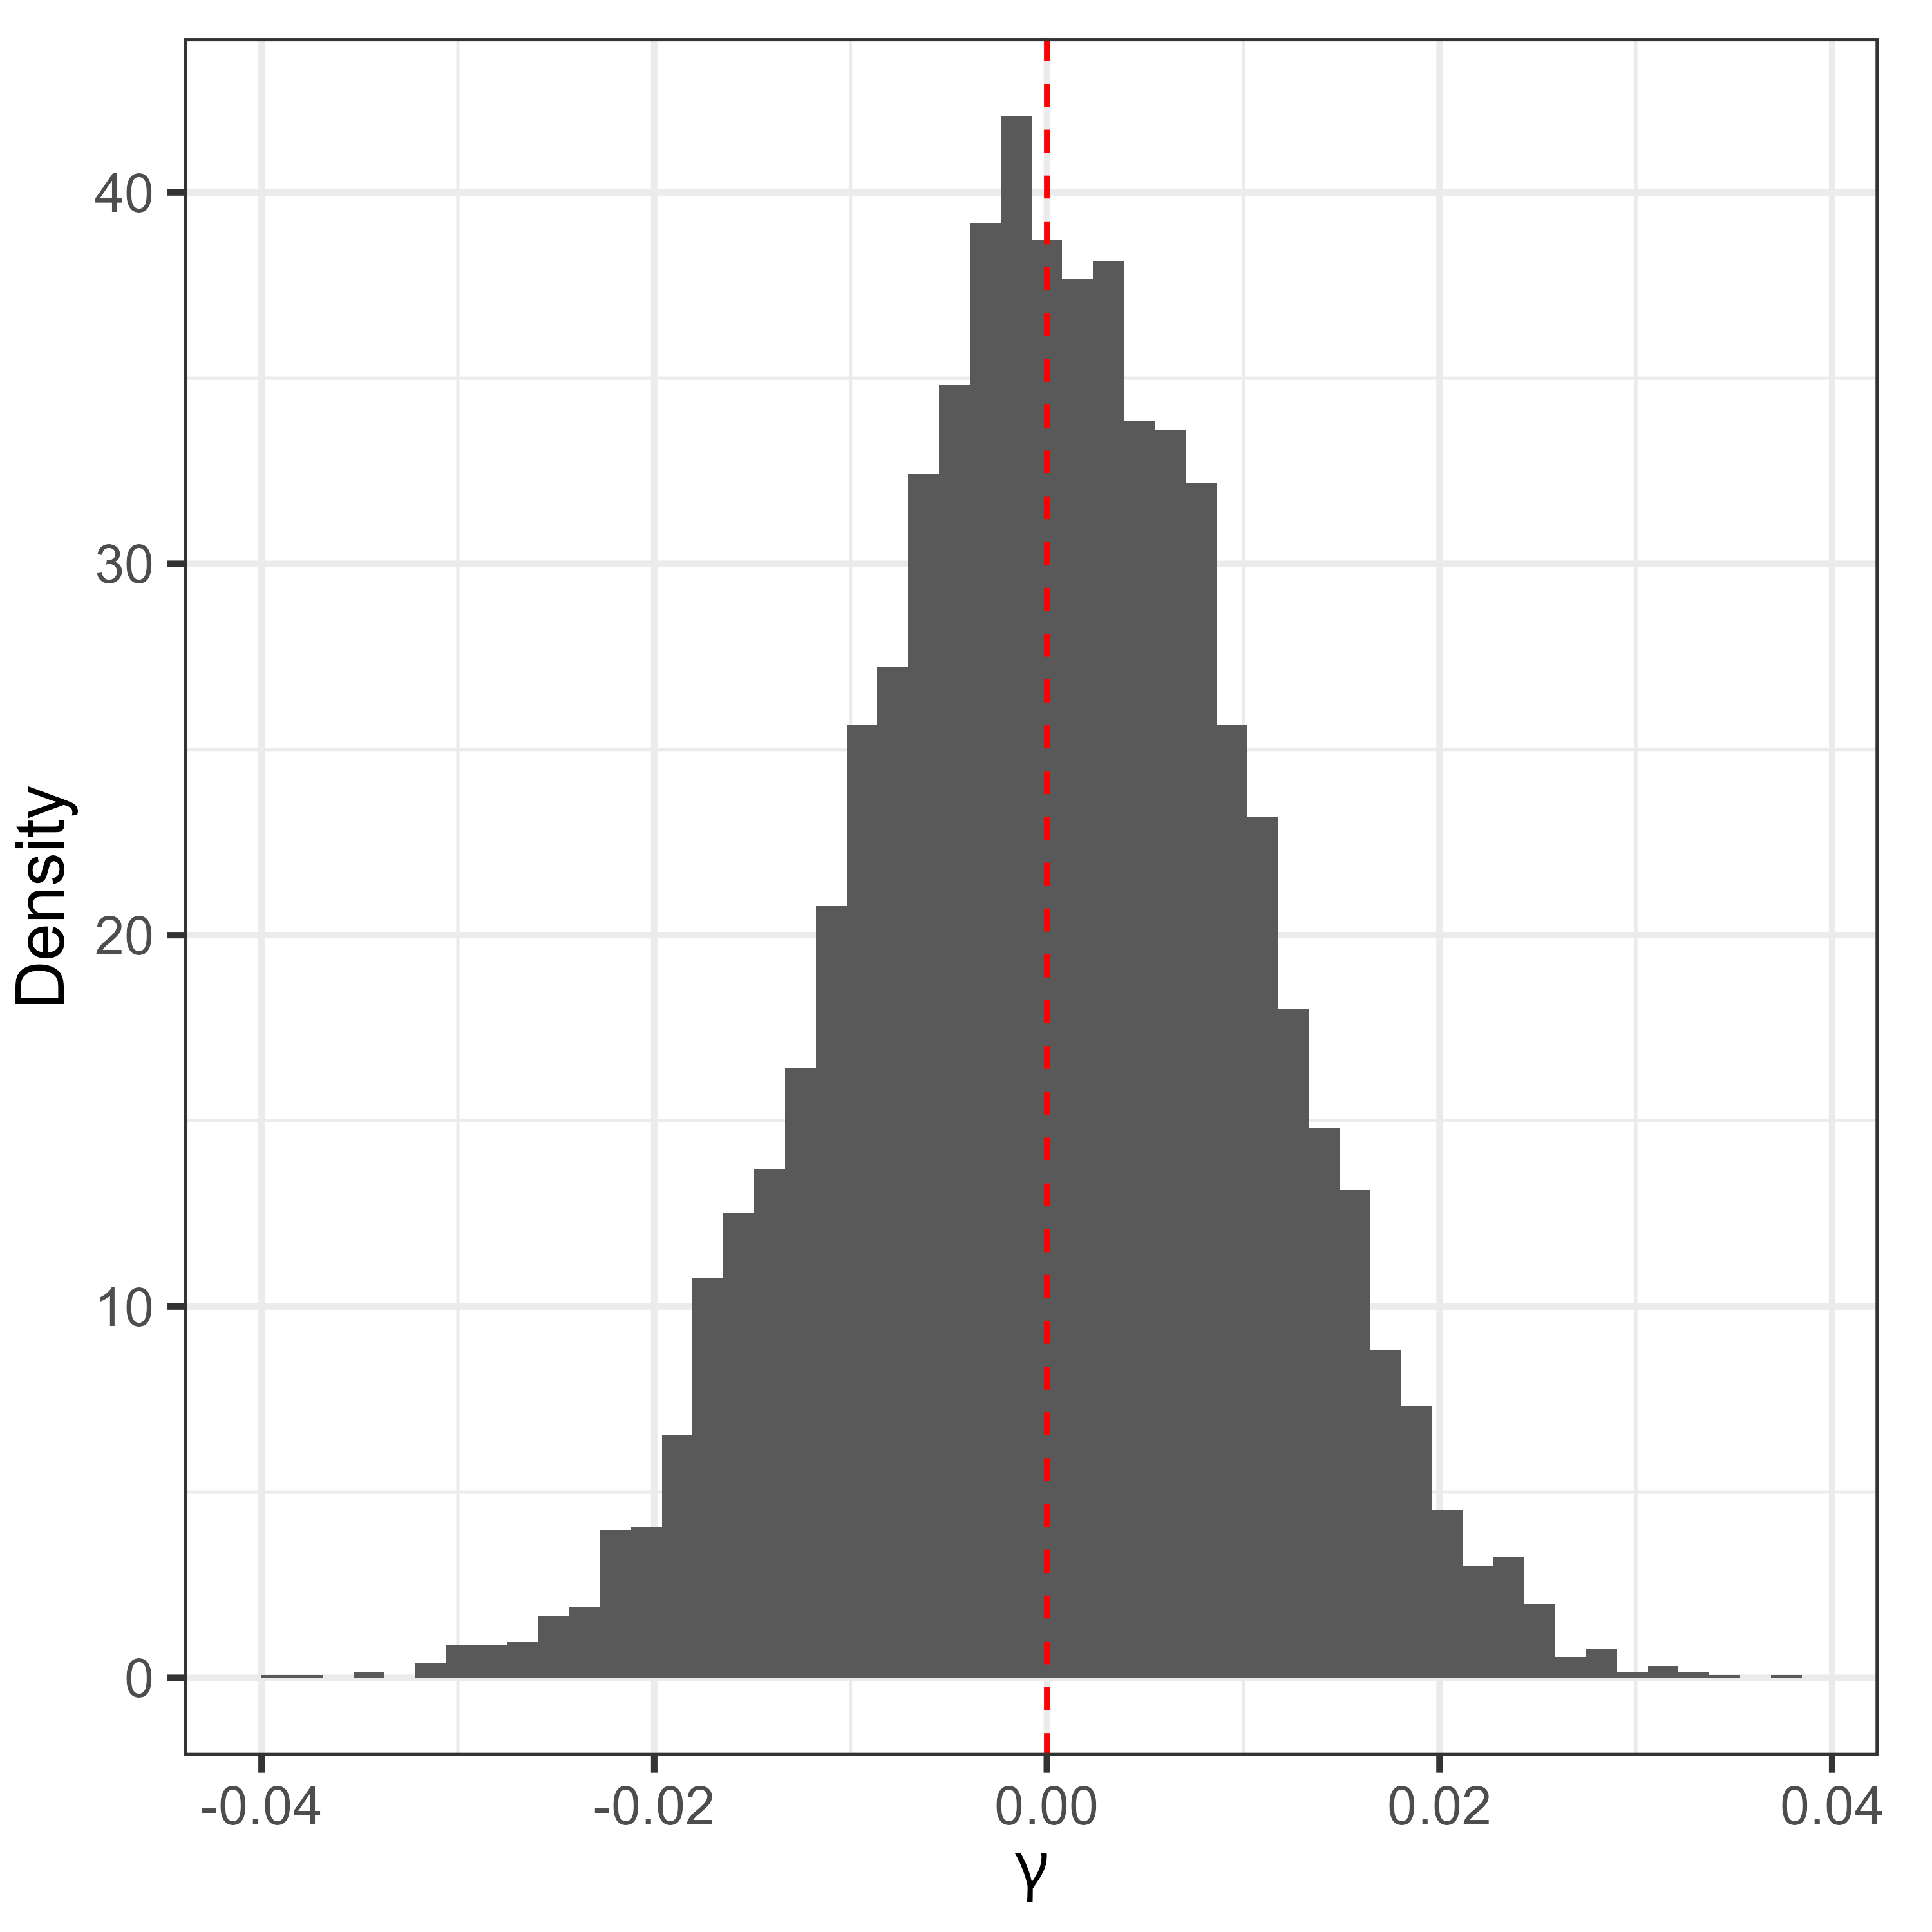
\includegraphics[width=0.45\textwidth]{../figures/simulation/hist_gamma.png}
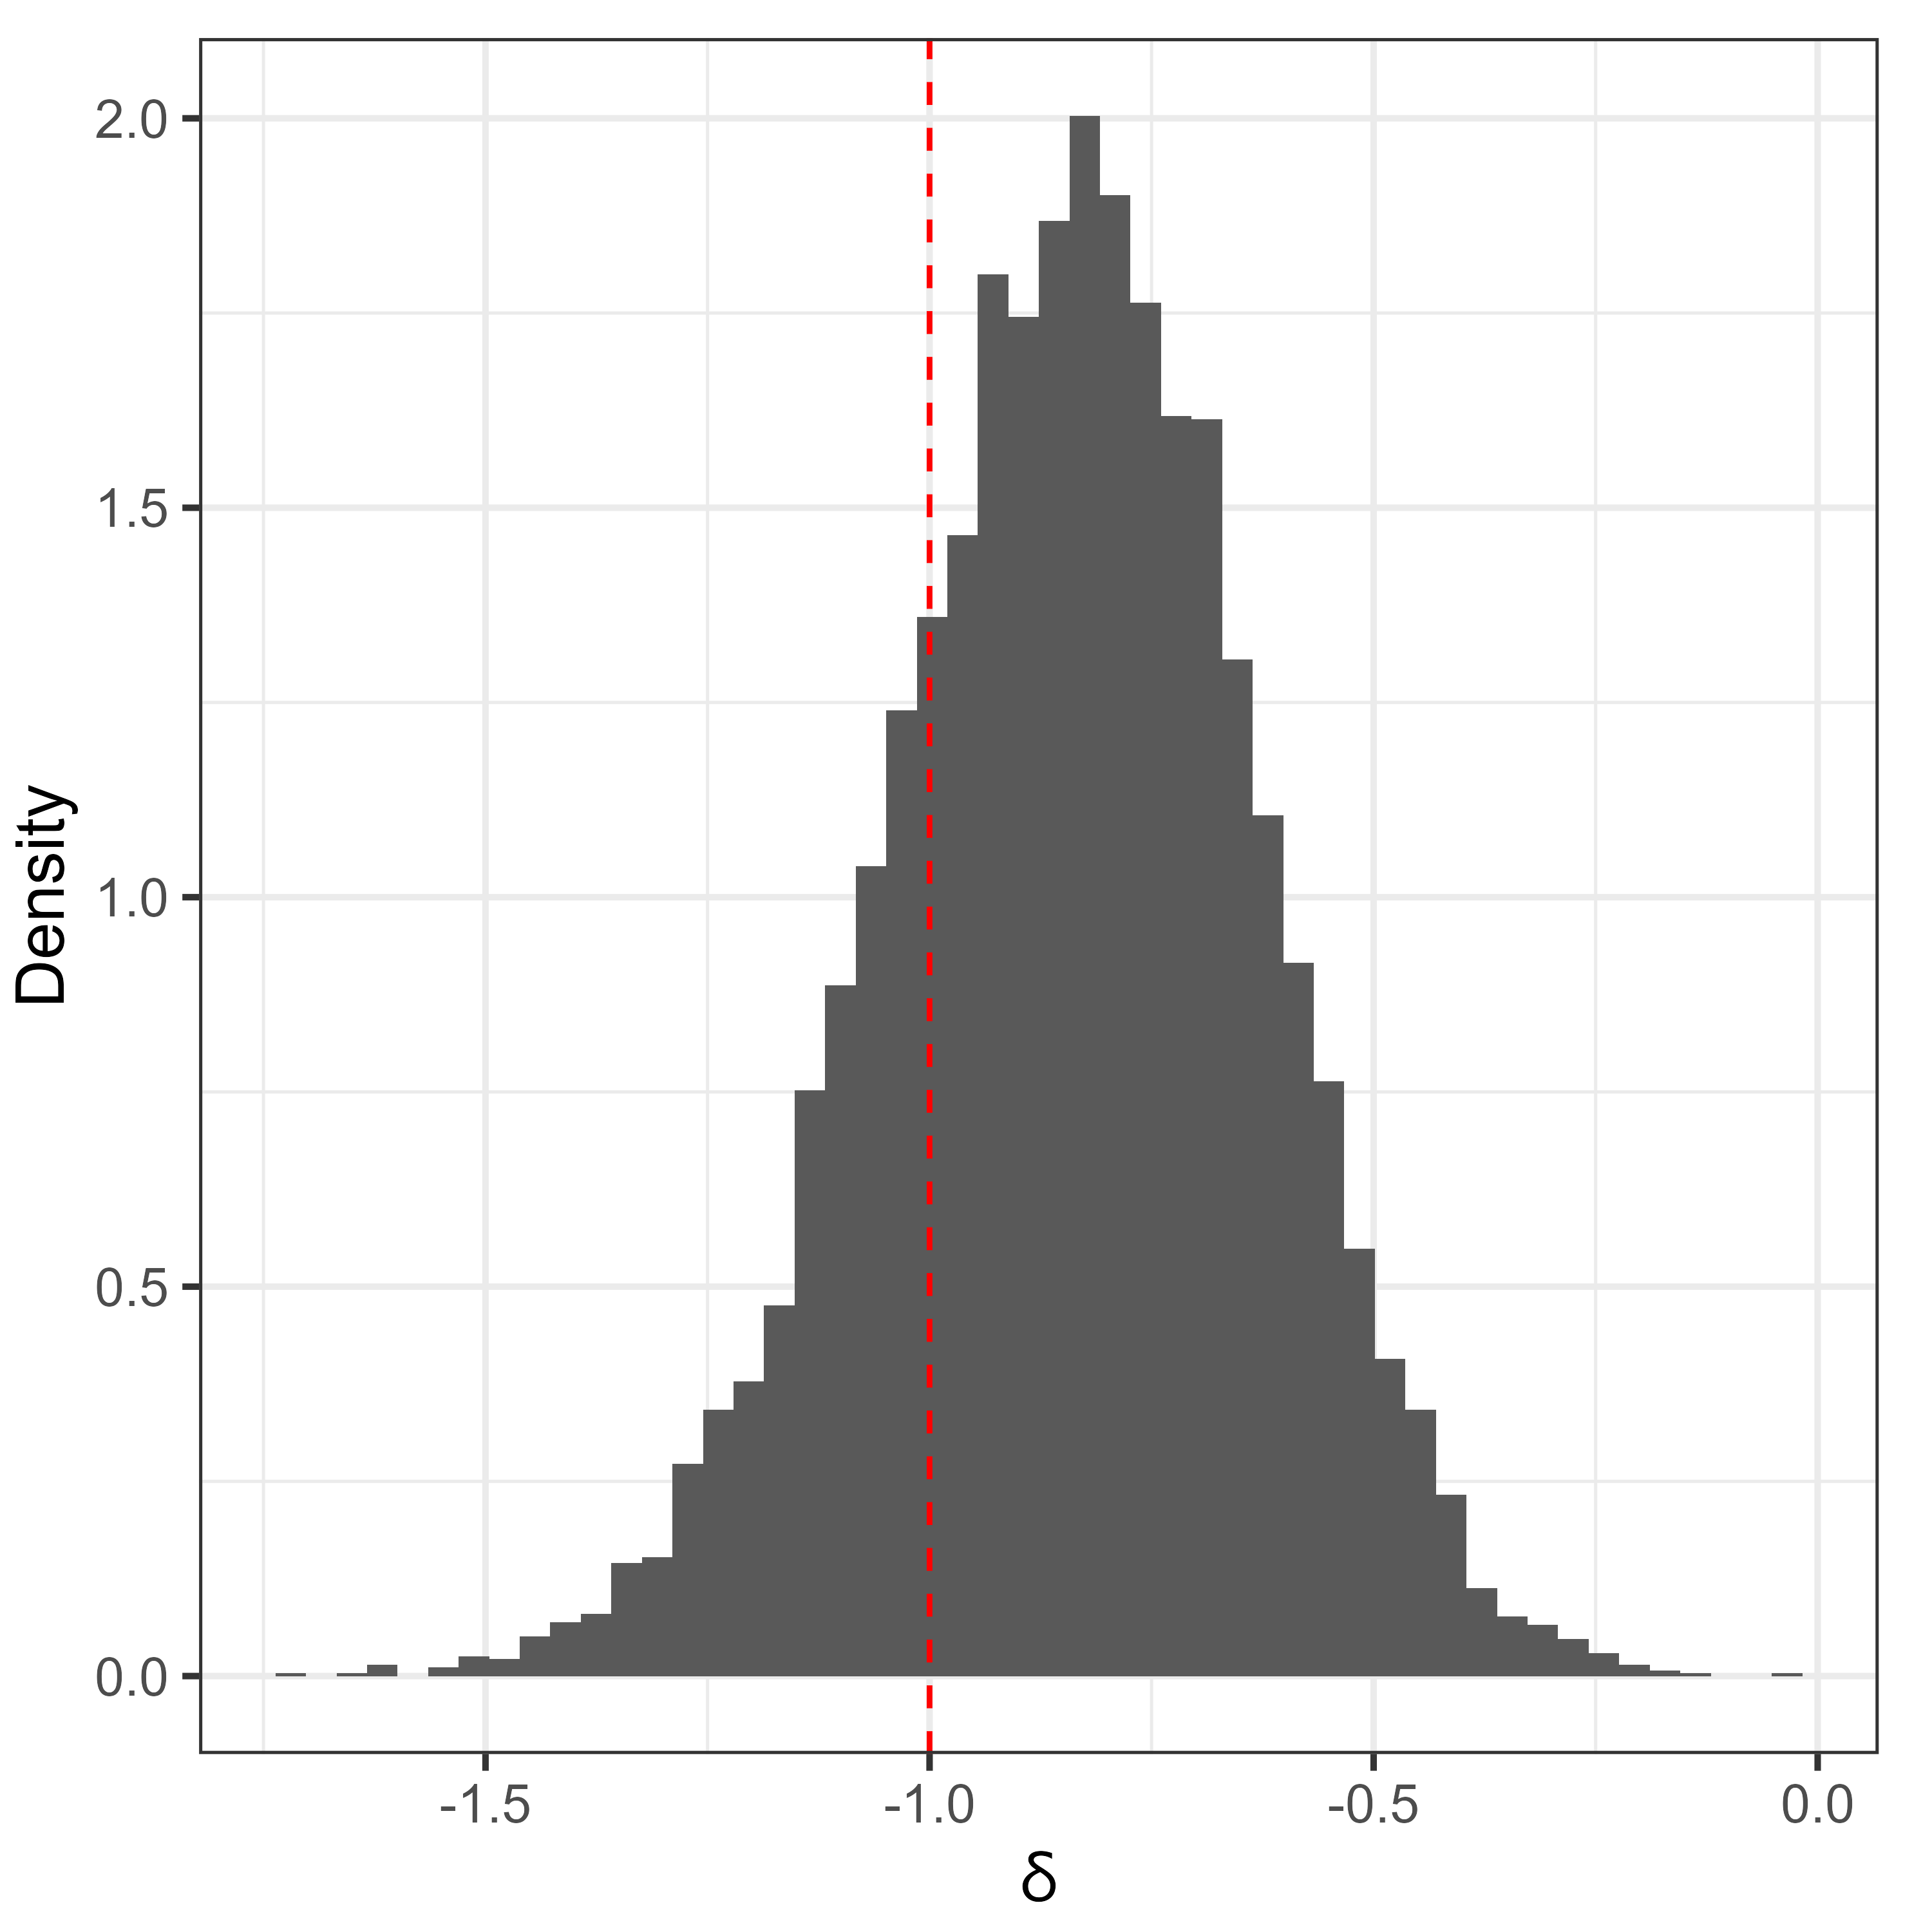
\includegraphics[width=0.45\textwidth]{../figures/simulation/hist_delta.png}
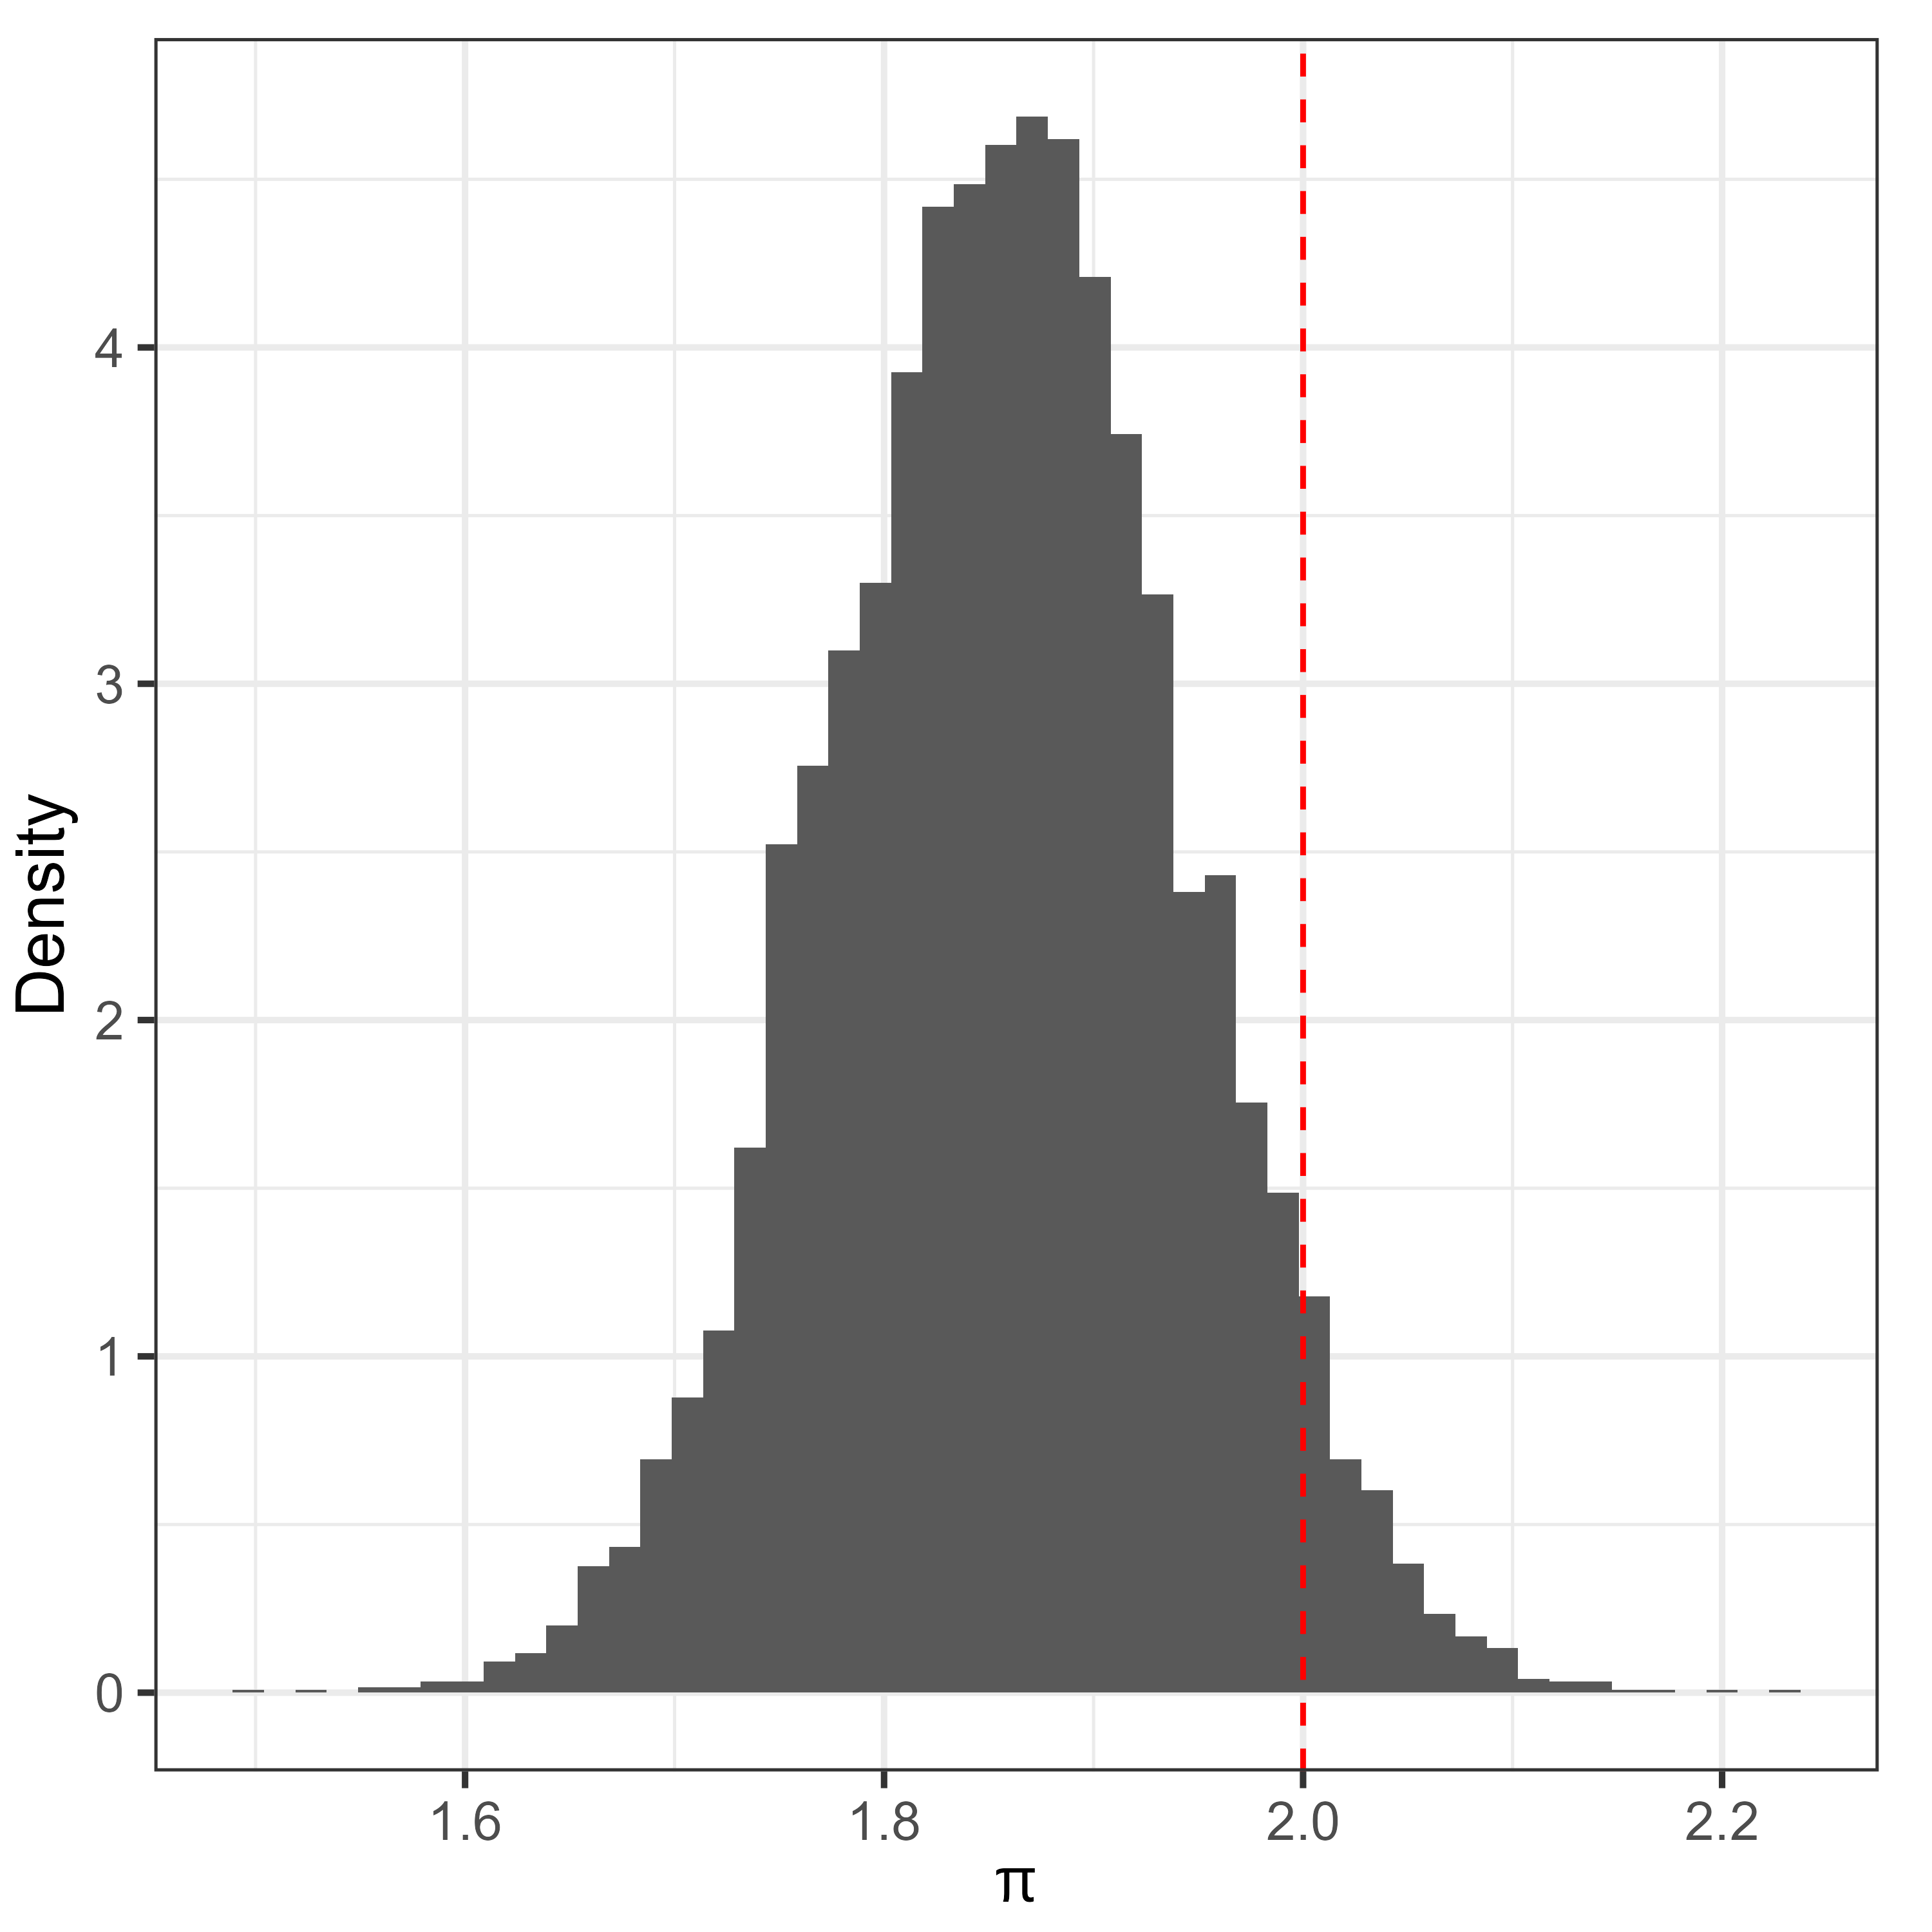
\includegraphics[width=0.45\textwidth]{../figures/simulation/hist_pi.png}
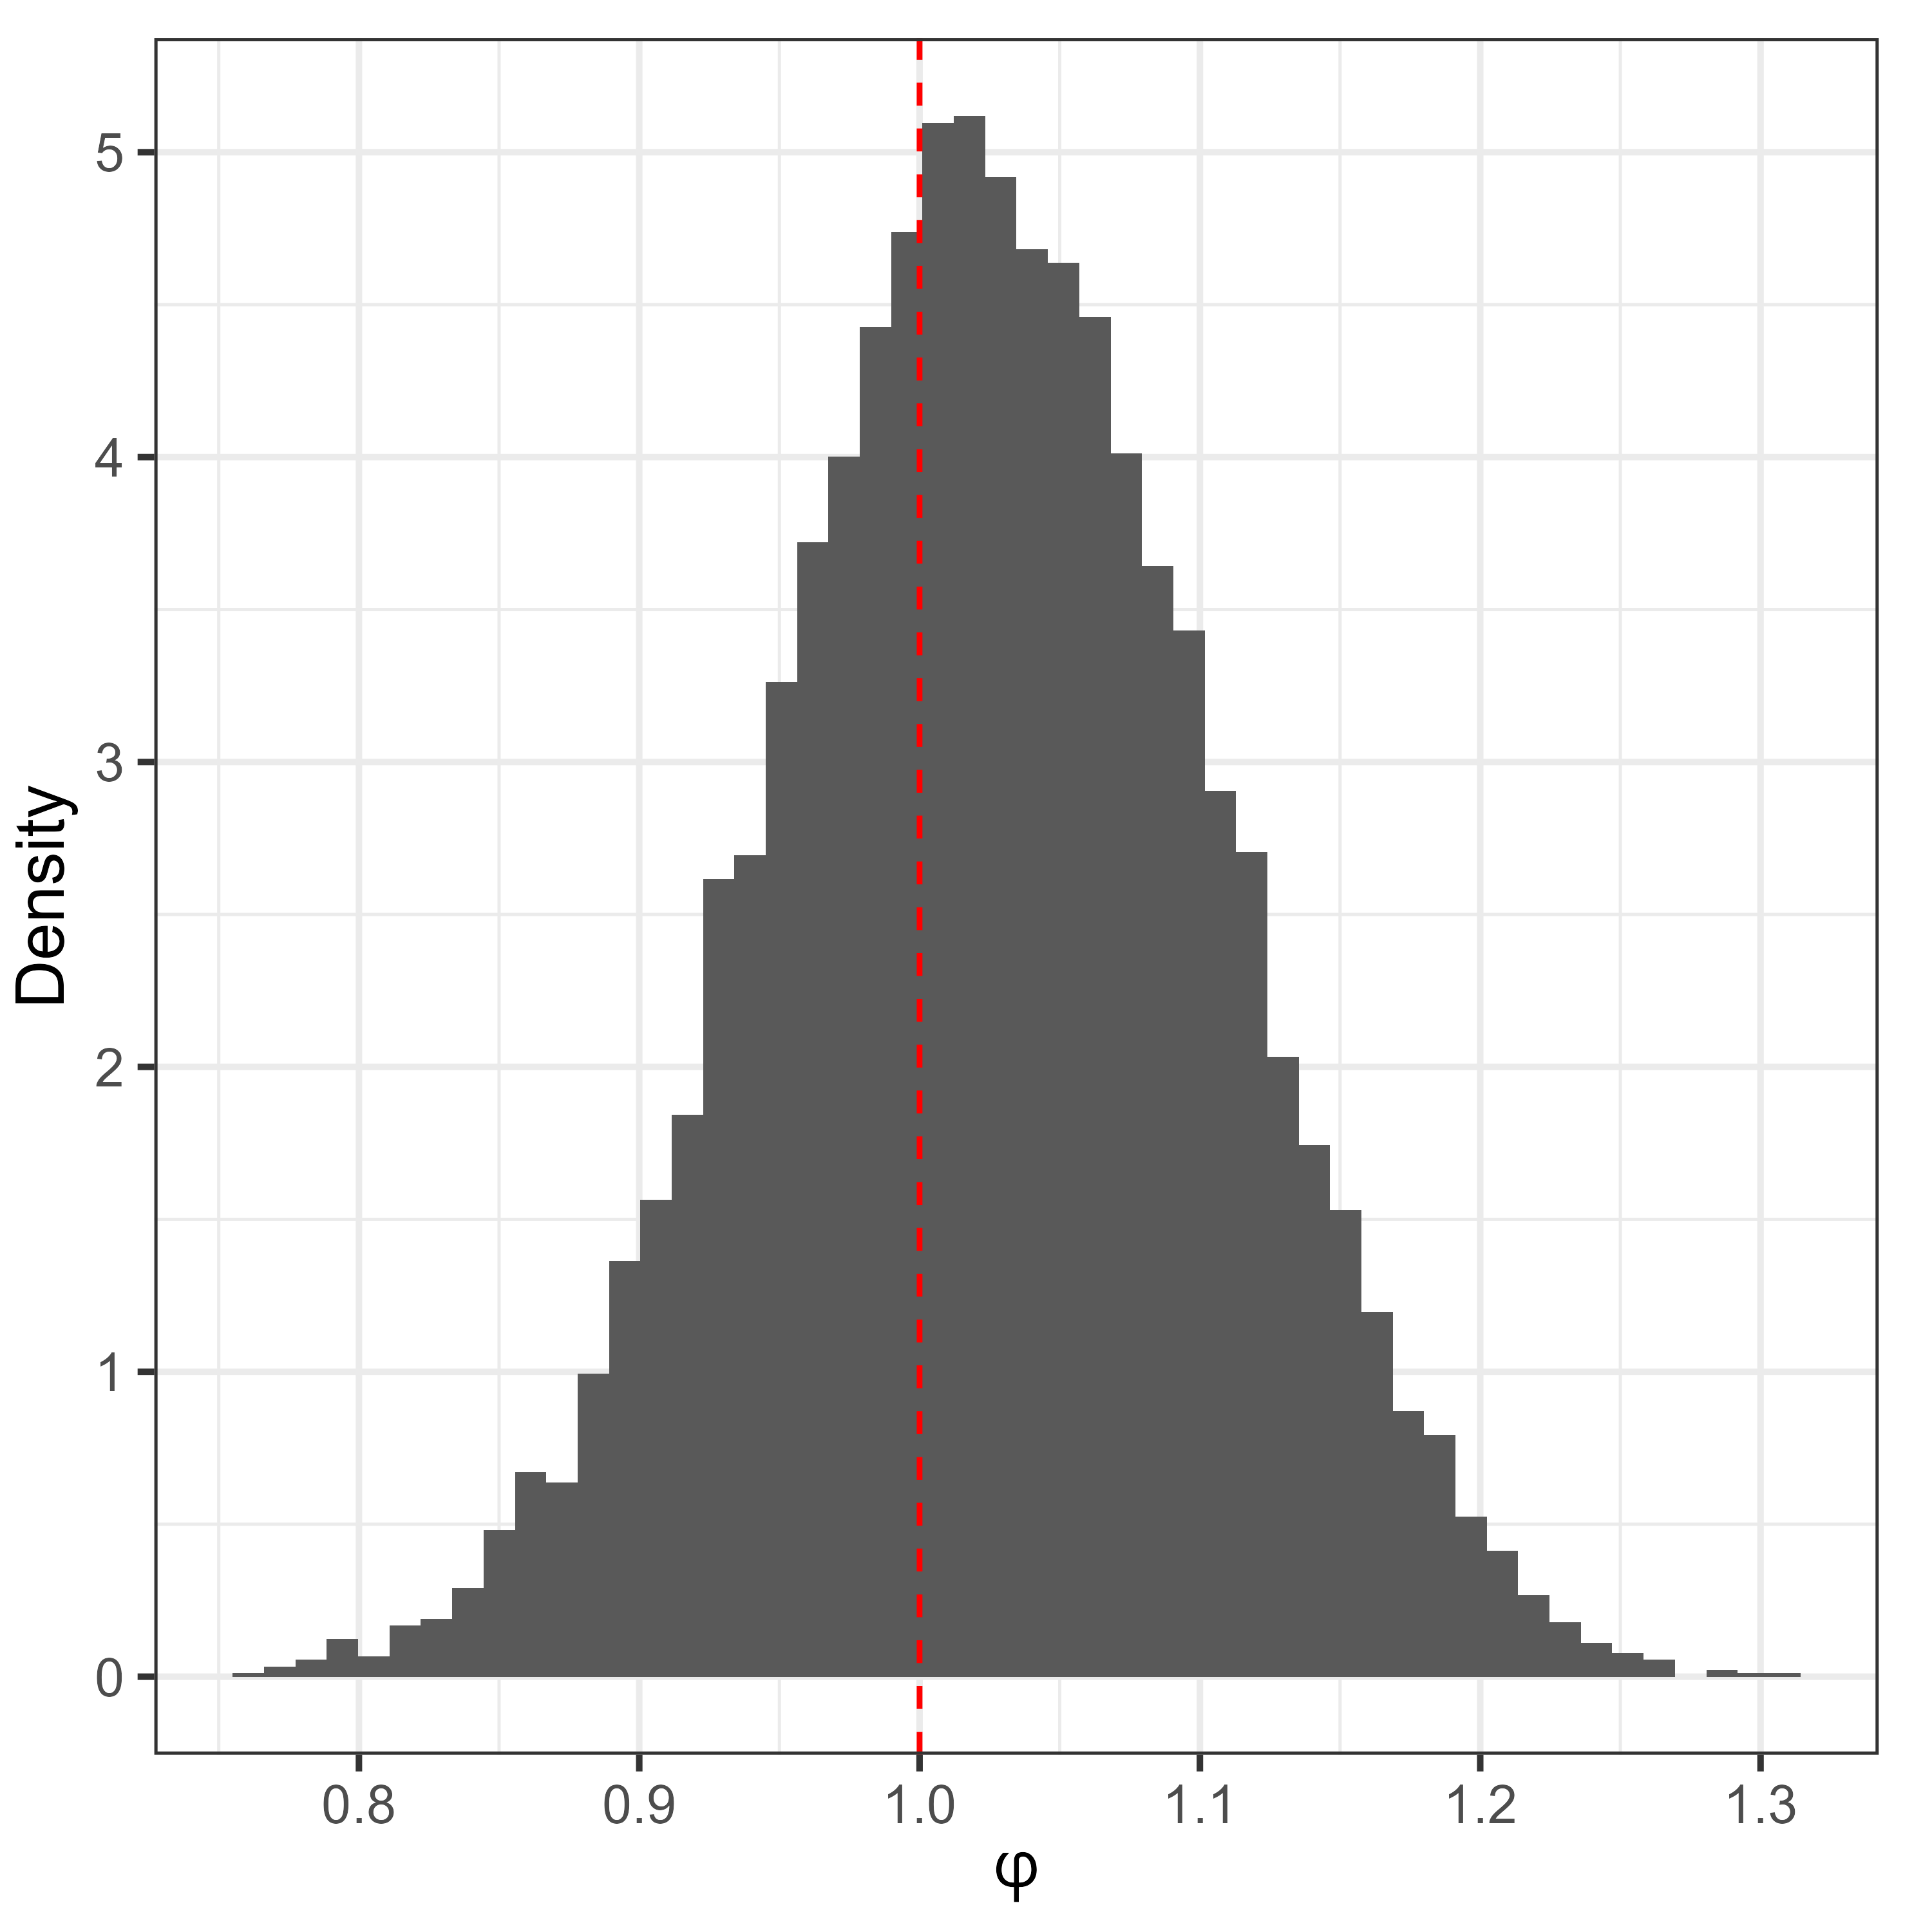
\includegraphics[width=0.45\textwidth]{../figures/simulation/hist_phi.png}
\caption{Posterior Distributions of $\gamma$, $\delta$, $\pi$, and $\phi$ --- Simulation Study}
\label{fig:posterior_distributions_2}
\end{figure}

This indicates that the Gibbs sampler is able to recover the true parameters of the model, even with a small sample size. As we parametrize the model with easy to sample priors and our Markov chain is well-behaved with a low autocorrelation, each additional sample is effectively independent. This can be seen in the Effective Sample Size (ESS) in Table \ref{tab:simulation_results}, which is close to the total number of samples, including for the $\beta$ variable a larger than 10,000 ESS as the autocorrelation for this variable is negative for some lags.

\subsection{Second Study}

For the second simulation exercise, we run three additional comparative analyses to assess the performance of the Bayesian plausibly exogenous model under different conditions. Specifically, we compare:

\begin{itemize}
    \item \textbf{Weak vs. Strong Instruments:} We vary the strength of the instrument by incorporating different noise levels in the data. 
    \item \textbf{Narrow vs. Wide Priors:} We compare results obtained under highly informative priors (small prior variance for $\gamma$) against results under weakly informative priors (large prior variance).
    \item \textbf{Valid vs. Invalid Instrument:} We contrast cases where the true value of $\gamma$ is zero (valid instrument) and where $\gamma$ is nonzero (invalid instrument).
\end{itemize}

For each scenario, we run the Gibbs sampler for $10{,}000$ iterations, discarding the first $5{,}000$ as burn-in. The posterior summary statistics for each setting are reported in Table \ref{tab:models}.


% Table created by stargazer v.5.2.3 by Marek Hlavac, Social Policy Institute. E-mail: marek.hlavac at gmail.com
% Date and time: Mon, Apr 28, 2025 - 11:48:21 PM
\begin{table}[!htbp] \centering 
  \caption{Simulation Results} 
  \label{tab:models} 
\begin{tabular}{@{\extracolsep{5pt}} ccccc} 
\\[-1.8ex]\hline 
\hline \\[-1.8ex] 
 & Mean & Standard Deviation & Lower CI & Upper CI \\ 
\hline \\[-1.8ex] 
Baseline & $2.03$ & $0.09$ & $1.85$ & $2.23$ \\ 
Weak Instrument & $0.16$ & $1.93$ & $$-$3.66$ & $4.20$ \\ 
Uncertain Instrument & $1.94$ & $0.52$ & $0.93$ & $2.97$ \\ 
Invalid Instrument & $7.04$ & $0.36$ & $6.37$ & $7.76$ \\ 
\hline \\[-1.8ex] 
\end{tabular} 
\end{table} 


\subsection{Third Study}
In this third simulation exercise, we conduct a sensitivity analysis by jointly varying the prior variance and the true value of $\gamma$, while examining the resulting posterior estimates of $\beta$. We focus initially on the case where the true $\gamma$ is fixed at $0$, and analyze how $\widehat{\beta}$ responds to different levels of prior informativeness regarding $\gamma$.

If the prior variance on $\gamma$ is set too small, the Bayesian procedure behaves similarly to imposing the sharp exclusion restriction $\gamma = 0$. In such cases, if $\gamma$ is not exactly zero, the estimator can suffer from omitted variable bias. Conversely, if the prior variance is set too large, the prior becomes weakly informative, approaching the behavior of ordinary least squares (OLS). In this limit, the estimator may lose precision and significance, because it allows for large direct effects of the instrument.

This exercise parallels the idea of \emph{sensitivity analysis}, as discussed in \cite{cinelliMakingSenseSensitivity2020}, where the robustness of causal conclusions to violations of identifying assumptions is systematically explored. In their paper, they propose a method to assess the sensitivity of causal conclusions to potential omitted variable bias. In our case, we are interested in the sensitivity of the posterior estimates of $\beta$ to the prior variance of $\gamma$.

The procedure follows the steps below:
\begin{itemize}
    \item Fix the true value of $\gamma$ (initially set to 0).
    \item Vary the prior variance of $\gamma$ across a wide grid of values, from highly informative (small variance) to weakly informative (large variance).
    \item For each specification, run the Gibbs sampler and record the posterior mean and credible interval for $\beta$.
\end{itemize}

The results are presented in Figure \ref{fig:sensitivity_analysis_beta}, which plots the posterior mean and credible intervals of $\beta$ against the log of the prior variance of $\gamma$.

\begin{figure}[H]
\centering
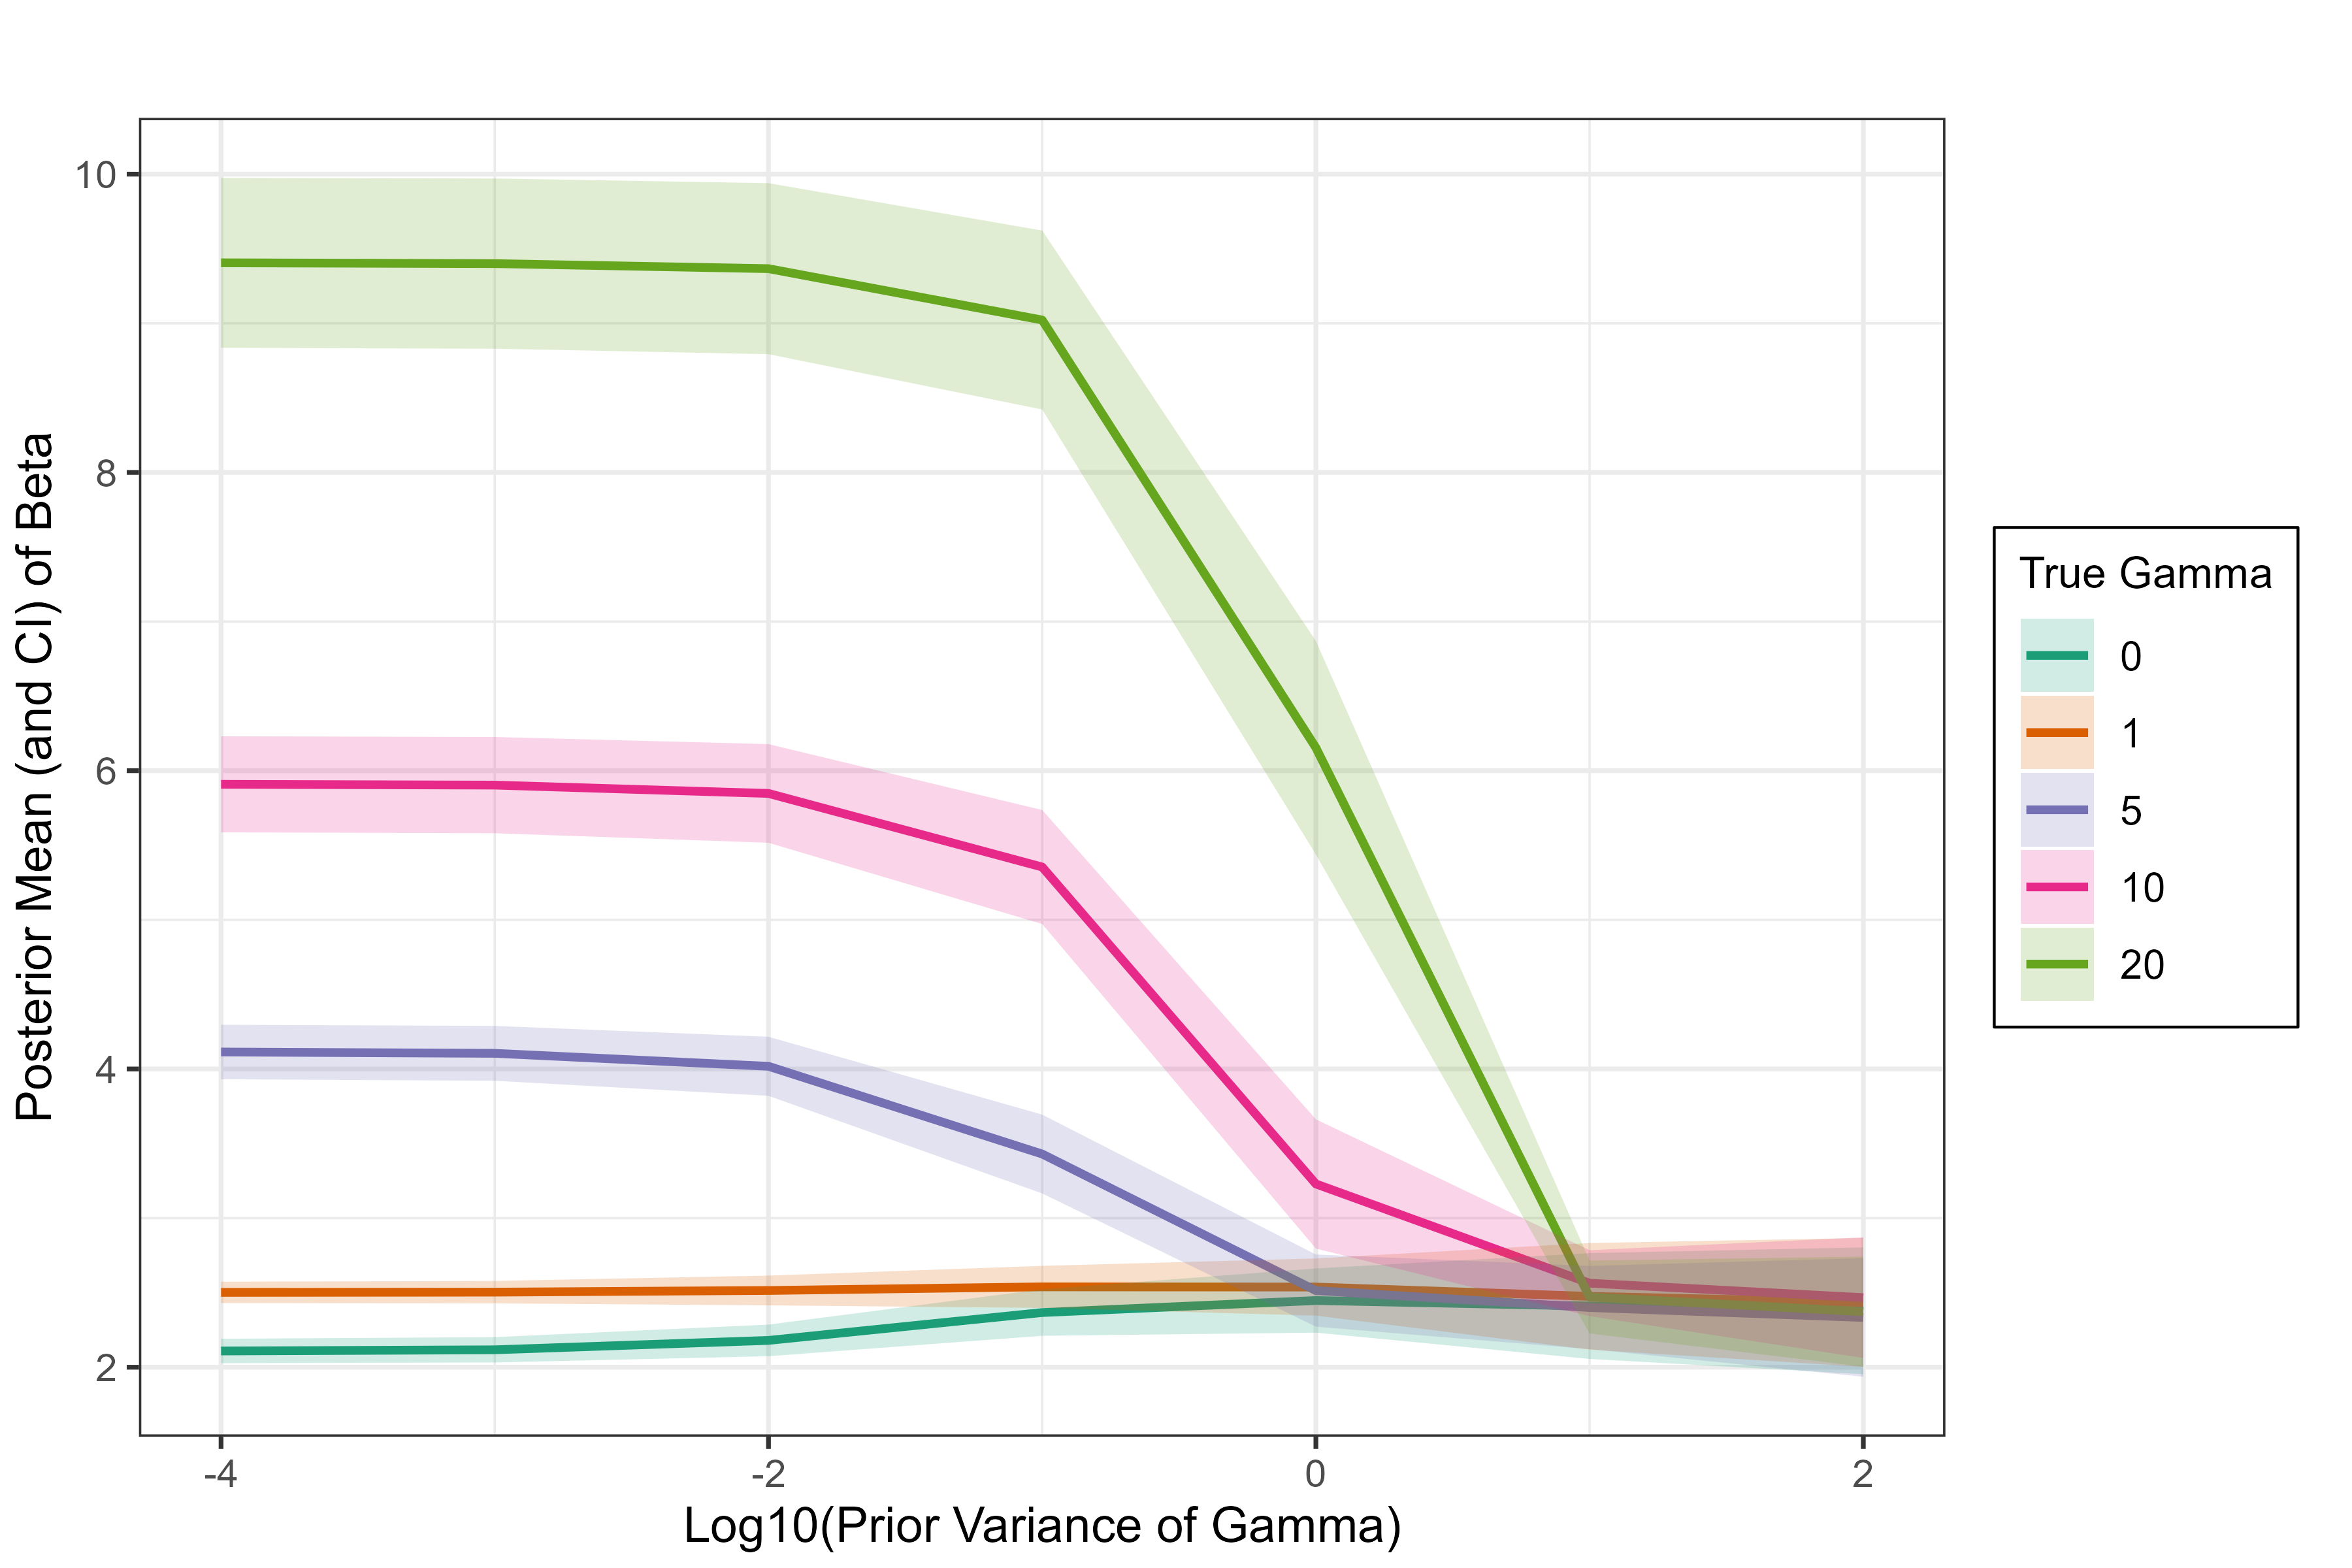
\includegraphics[width=0.9\textwidth]{../figures/simulation/plot_prior_gamma.png}
\caption{Sensitivity Analysis of $\widehat{\beta}$ to Prior Variance of $\gamma$ --- Simulation Study}
\label{fig:sensitivity_analysis_beta}
\end{figure}

As we can see, when the prior variance is very small, we firmly believe that $\gamma$ is equal to 0, and the posterior mean of $\beta$ is close to the true value. If this were to be false, we would be far away from $\beta$ true value, as occurs for different values of $\gamma$. However, as we impose a less informative prior, by increasing the prior variance of $\gamma$, allowing for a non-zero coefficient for the instrument, we see that the posterior mean of $\beta$ converge to a biased estimate which is the same for all true values of $\gamma$. This is because the prior variance is so large that it dominates the likelihood, and the posterior mean of $\beta$ is driven by the prior.  
\section{Replication}

The paper by \cite{acemogluColonialOriginsComparative2001} studies the impact of colonialism on economic development. The authors employ a two-stage least squares (2SLS) approach to estimate the causal effect of early institutions on current economic performance. Specifically, they use historical data on settler mortality as an instrument for institutional quality, arguing that areas with higher settler mortality rates developed extractive institutions, which persisted and adversely affected modern economic outcomes. 

The structural relationship they estimate can be summarized as:
\begin{align*}
    \text{log GDP per capita} &= \beta \times \text{Expropriation Risk} + \varepsilon,
\end{align*}
where Expropriation Risk is instrumented by historical Settler Mortality.

The identification strategy relies on the assumption that settler mortality affects current income only through its effect on institutions, and not through other channels. In other words, settler mortality must be excluded from the structural equation for income, satisfying the exclusion restriction $\gamma = 0$.

However, this assumption has been the subject of debate. \cite{albouyColonialOriginsComparative2012} criticizes the original study by arguing that the measurement of settler mortality is problematic and that the sample of colonies used by \cite{acemogluColonialOriginsComparative2001} may introduce biases. He also points out that settler mortality could directly influence current development outcomes through channels unrelated to institutions, thereby violating the exclusion restriction.

Additionally, \cite{glaeserInstitutionsCauseGrowth2004} question the broader framework, suggesting that human capital, rather than institutions per se, may be the more fundamental driver of economic growth. If this critique holds, settler mortality could directly affect economic outcomes by shaping human capital accumulation, again violating the exclusion assumption.

Given these concerns, applying the Bayesian plausibly exogenous framework of \cite{conleyPlausiblyExogenous2012} to the \cite{acemogluColonialOriginsComparative2001} dataset provides a natural way to assess the robustness of the original findings. By allowing for a nonzero but small direct effect of settler mortality, we can explore how sensitive the estimated causal effect of institutions is to plausible violations of the exclusion restriction.

Thus, we can apply the Bayesian approach developed in the previous section to the dataset used by \cite{acemogluColonialOriginsComparative2001}. 

We specify the prior for the coefficient on the instrument ($\gamma$) with mean zero, reflecting the belief in approximate exclusion, and for the intercept term and the coefficient on the exogenous variable ($\delta$) we use the sample mean of the corresponding variable. For the prior variances, we follow the 2-$\sigma$ rule for the level coefficient and set the prior variance for the coefficient on the instrument to $10$. 

We run the Gibbs sampler for $10{,}000$ iterations, discarding the first $2{,}000$ as burn-in. The posterior summary statistics are reported in Table \ref{tab:replication_results}.


% Table created by stargazer v.5.2.3 by Marek Hlavac, Social Policy Institute. E-mail: marek.hlavac at gmail.com
% Date and time: Mon, Apr 28, 2025 - 11:55:52 PM
\begin{table}[!htbp] \centering 
  \caption{Replication Results} 
  \label{tab:replication_results} 
\begin{tabular}{@{\extracolsep{5pt}} ccccccc} 
\\[-1.8ex]\hline 
\hline \\[-1.8ex] 
Parameter & True Value & Mean & Standard Deviation & 0.025 & 0.975 & Effective Sample Size \\ 
\hline \\[-1.8ex] 
pi & -0.61 & $$-$0.58$ & $0.12$ & $$-$0.82$ & $$-$0.33$ & $6,830.29$ \\ 
phi & - & $9.21$ & $0.59$ & $8.02$ & $10.37$ & $6,751.66$ \\ 
beta & 0.94 & $0.92$ & $0.25$ & $0.50$ & $1.45$ & $13,644.54$ \\ 
gamma & 0 & $$-$0.00$ & $0.01$ & $$-$0.02$ & $0.02$ & $6,881.64$ \\ 
delta & - & $2.10$ & $1.61$ & $$-$1.40$ & $4.81$ & $13,646.41$ \\ 
\hline \\[-1.8ex] 
\end{tabular} 
\end{table} 


The true value is referencing the value of the parameter in Table 4 from \cite{acemogluColonialOriginsComparative2001}. The posterior mean and credible intervals are close to the frequentist estimates, indicating that the Bayesian model is able to recover the frequentist estimates. 

The traceplot in Figure \ref{fig:replication_traceplot} illustrates the convergence of the Gibbs sampler. We observe no discernible patterns, suggesting the Markov chain has mixed well and reached stationarity.

\begin{figure}[H]
\centering
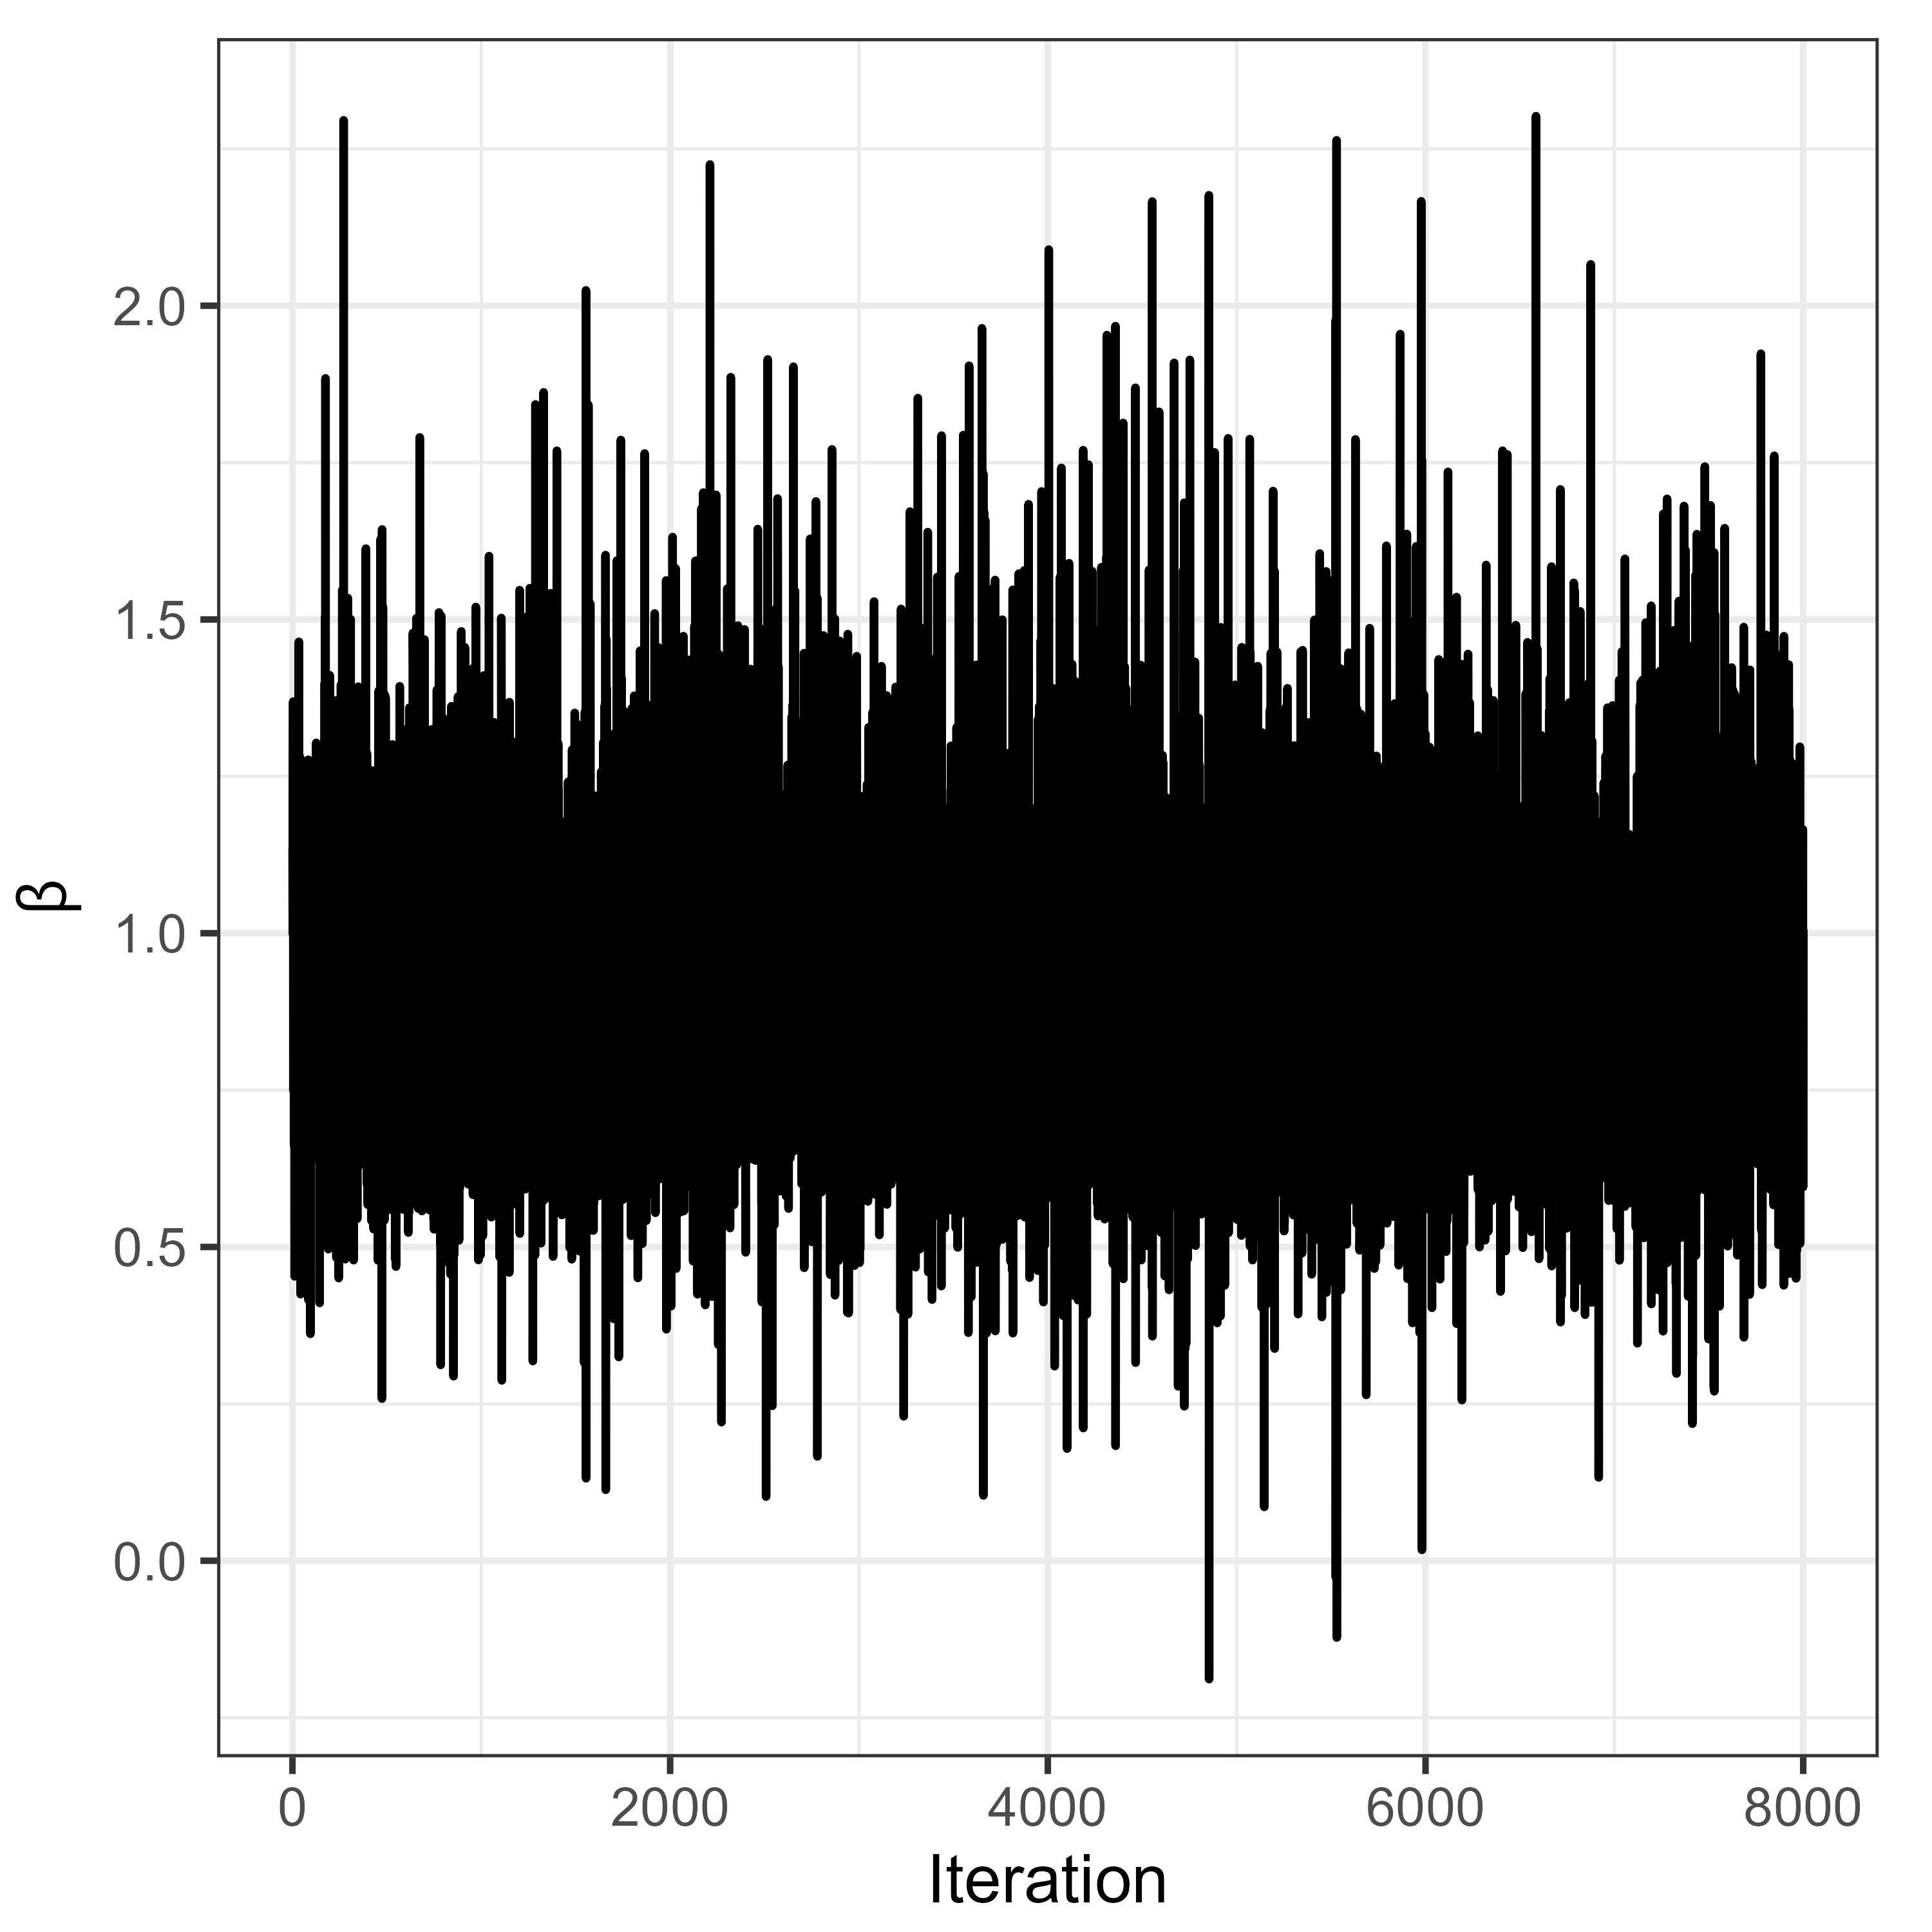
\includegraphics[width=0.8\textwidth]{../figures/acemoglu/trace_beta.png}
\caption{Traceplot of $\beta$ --- Replication Study}
\label{fig:replication_traceplot}
\end{figure}

The autocorrelation plot in Figure \ref{fig:replication_autocorrelation} shows low autocorrelation at all lags, reinforcing the evidence of good mixing and approximate independence across draws.

\begin{figure}[H]
\centering
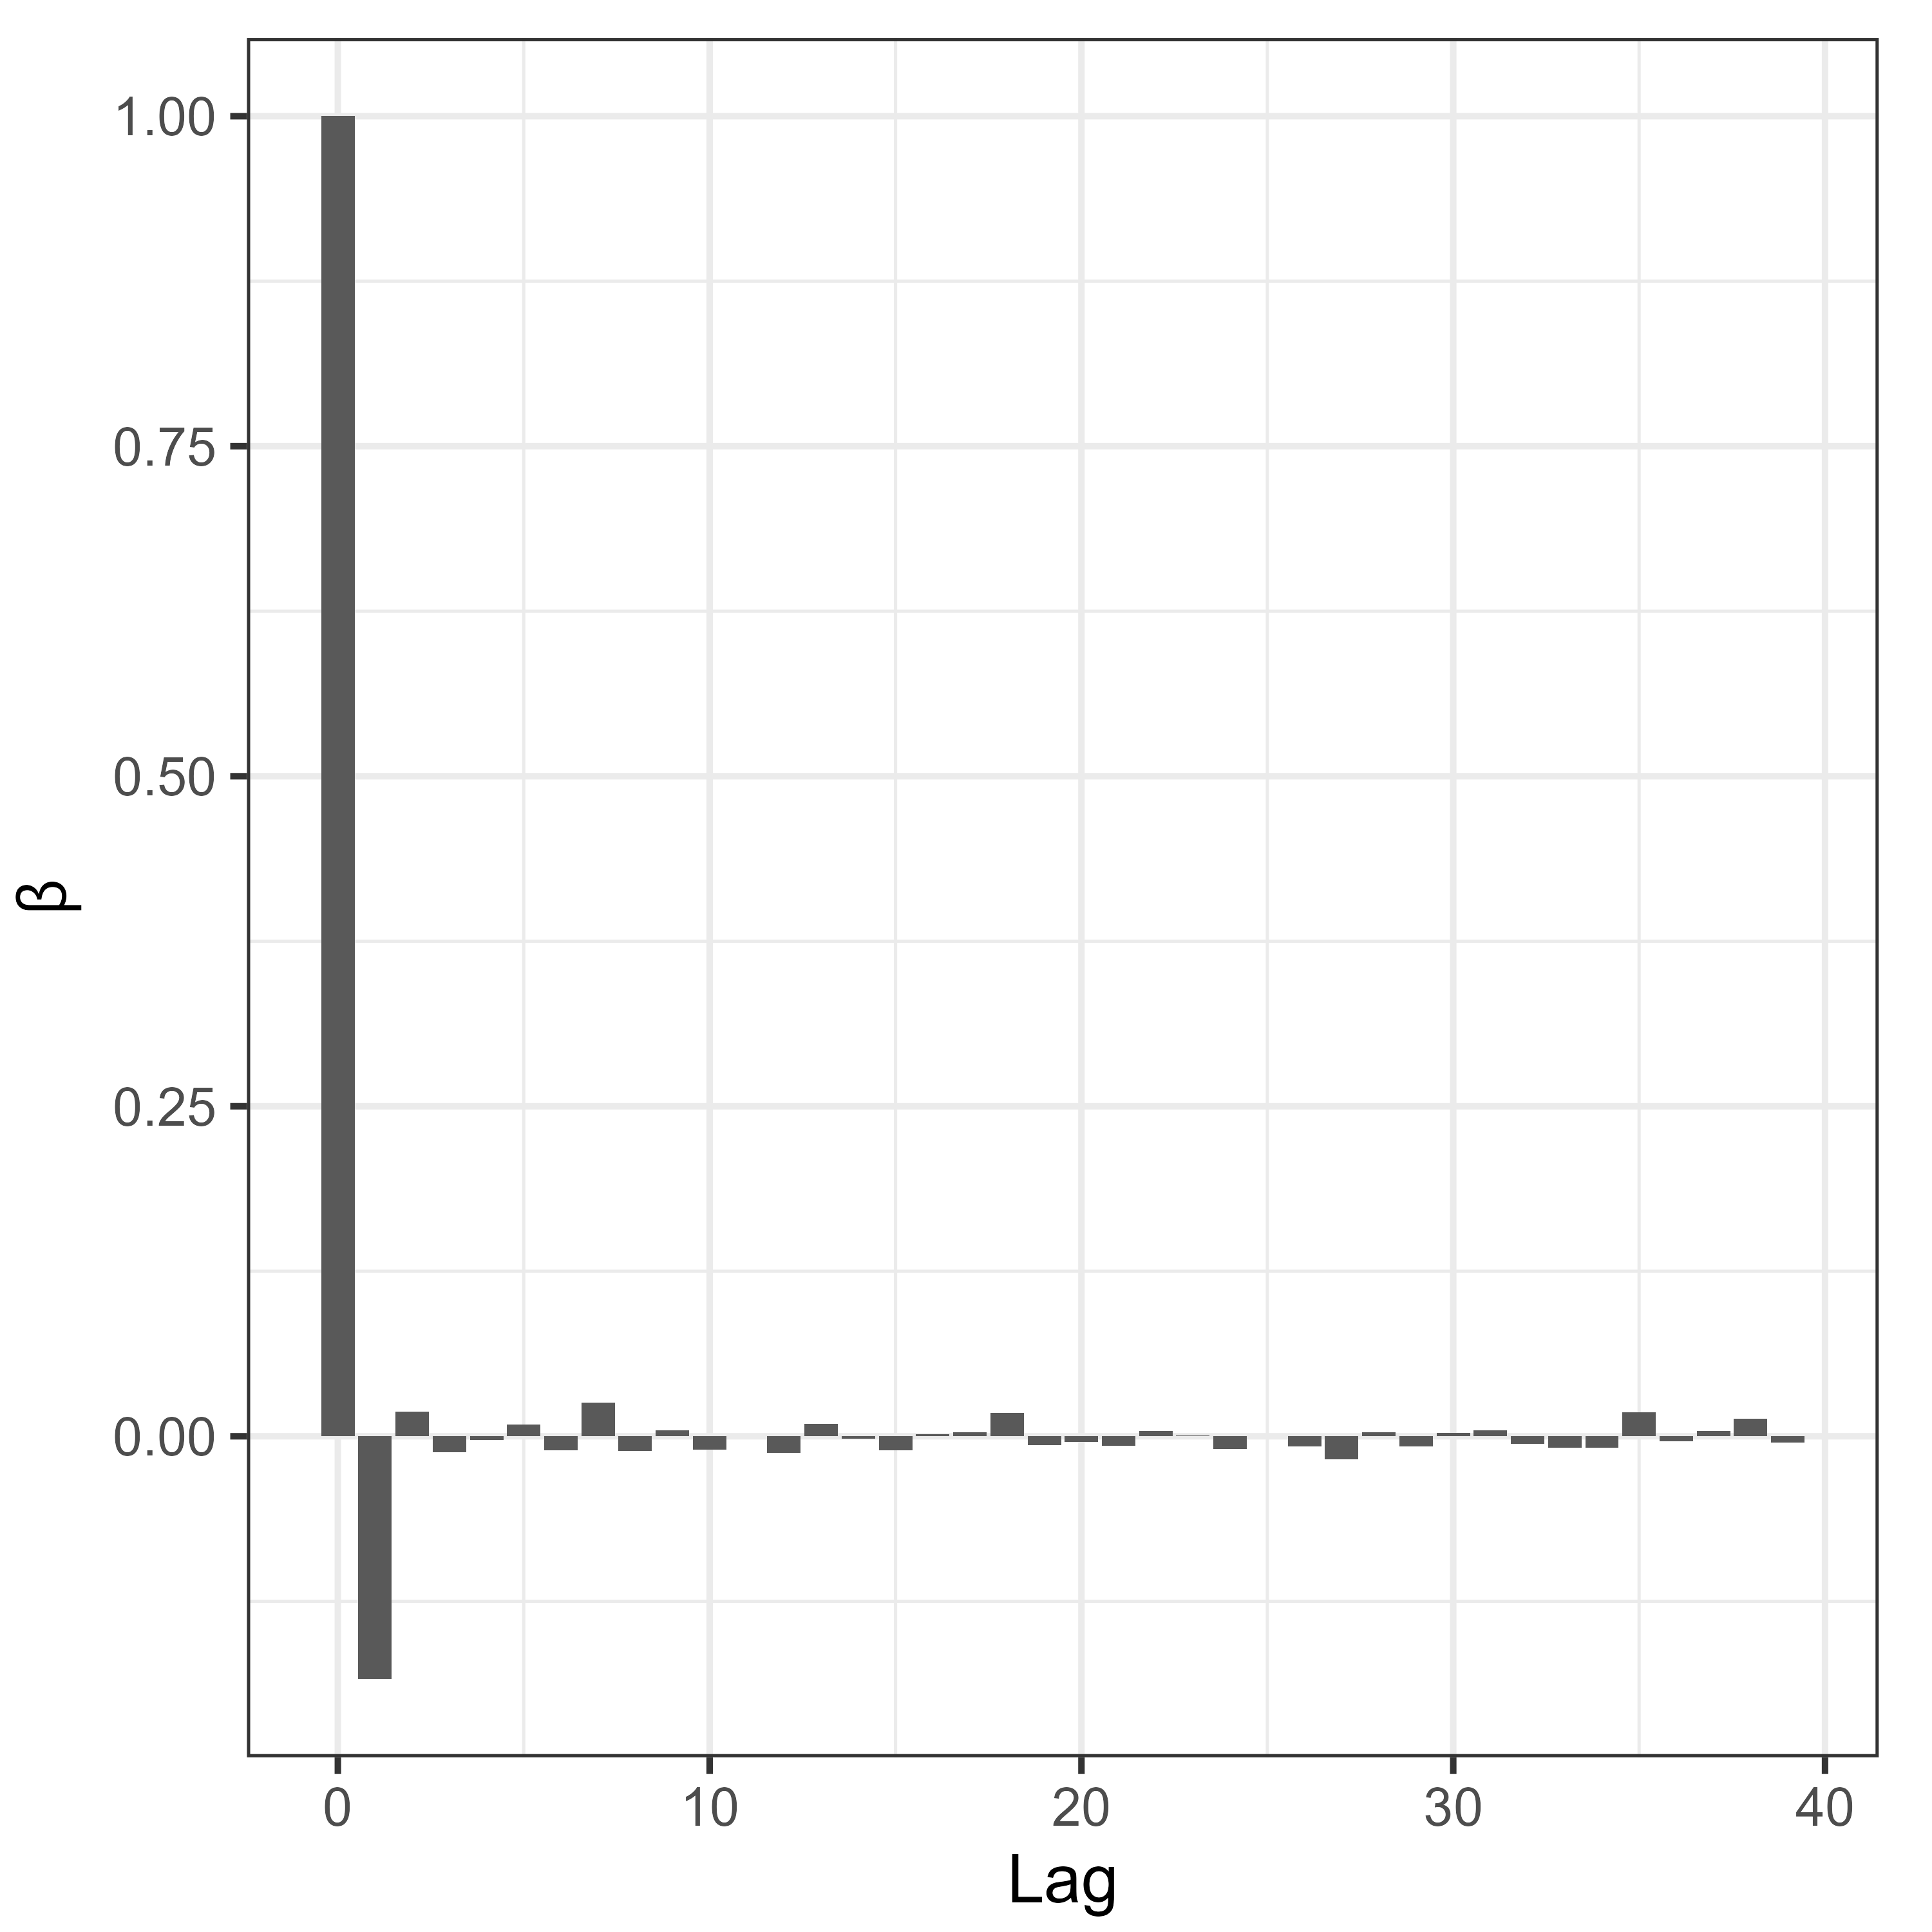
\includegraphics[width=0.8\textwidth]{../figures/acemoglu/acf_beta.png}
\caption{Autocorrelation of $\beta$ --- Replication Study}
\label{fig:replication_autocorrelation}
\end{figure}

We also present the posterior distributions of the parameters in Figure \ref{fig:replication_posterior_distributions}, visualized as histograms.

\begin{figure}[H]
\centering
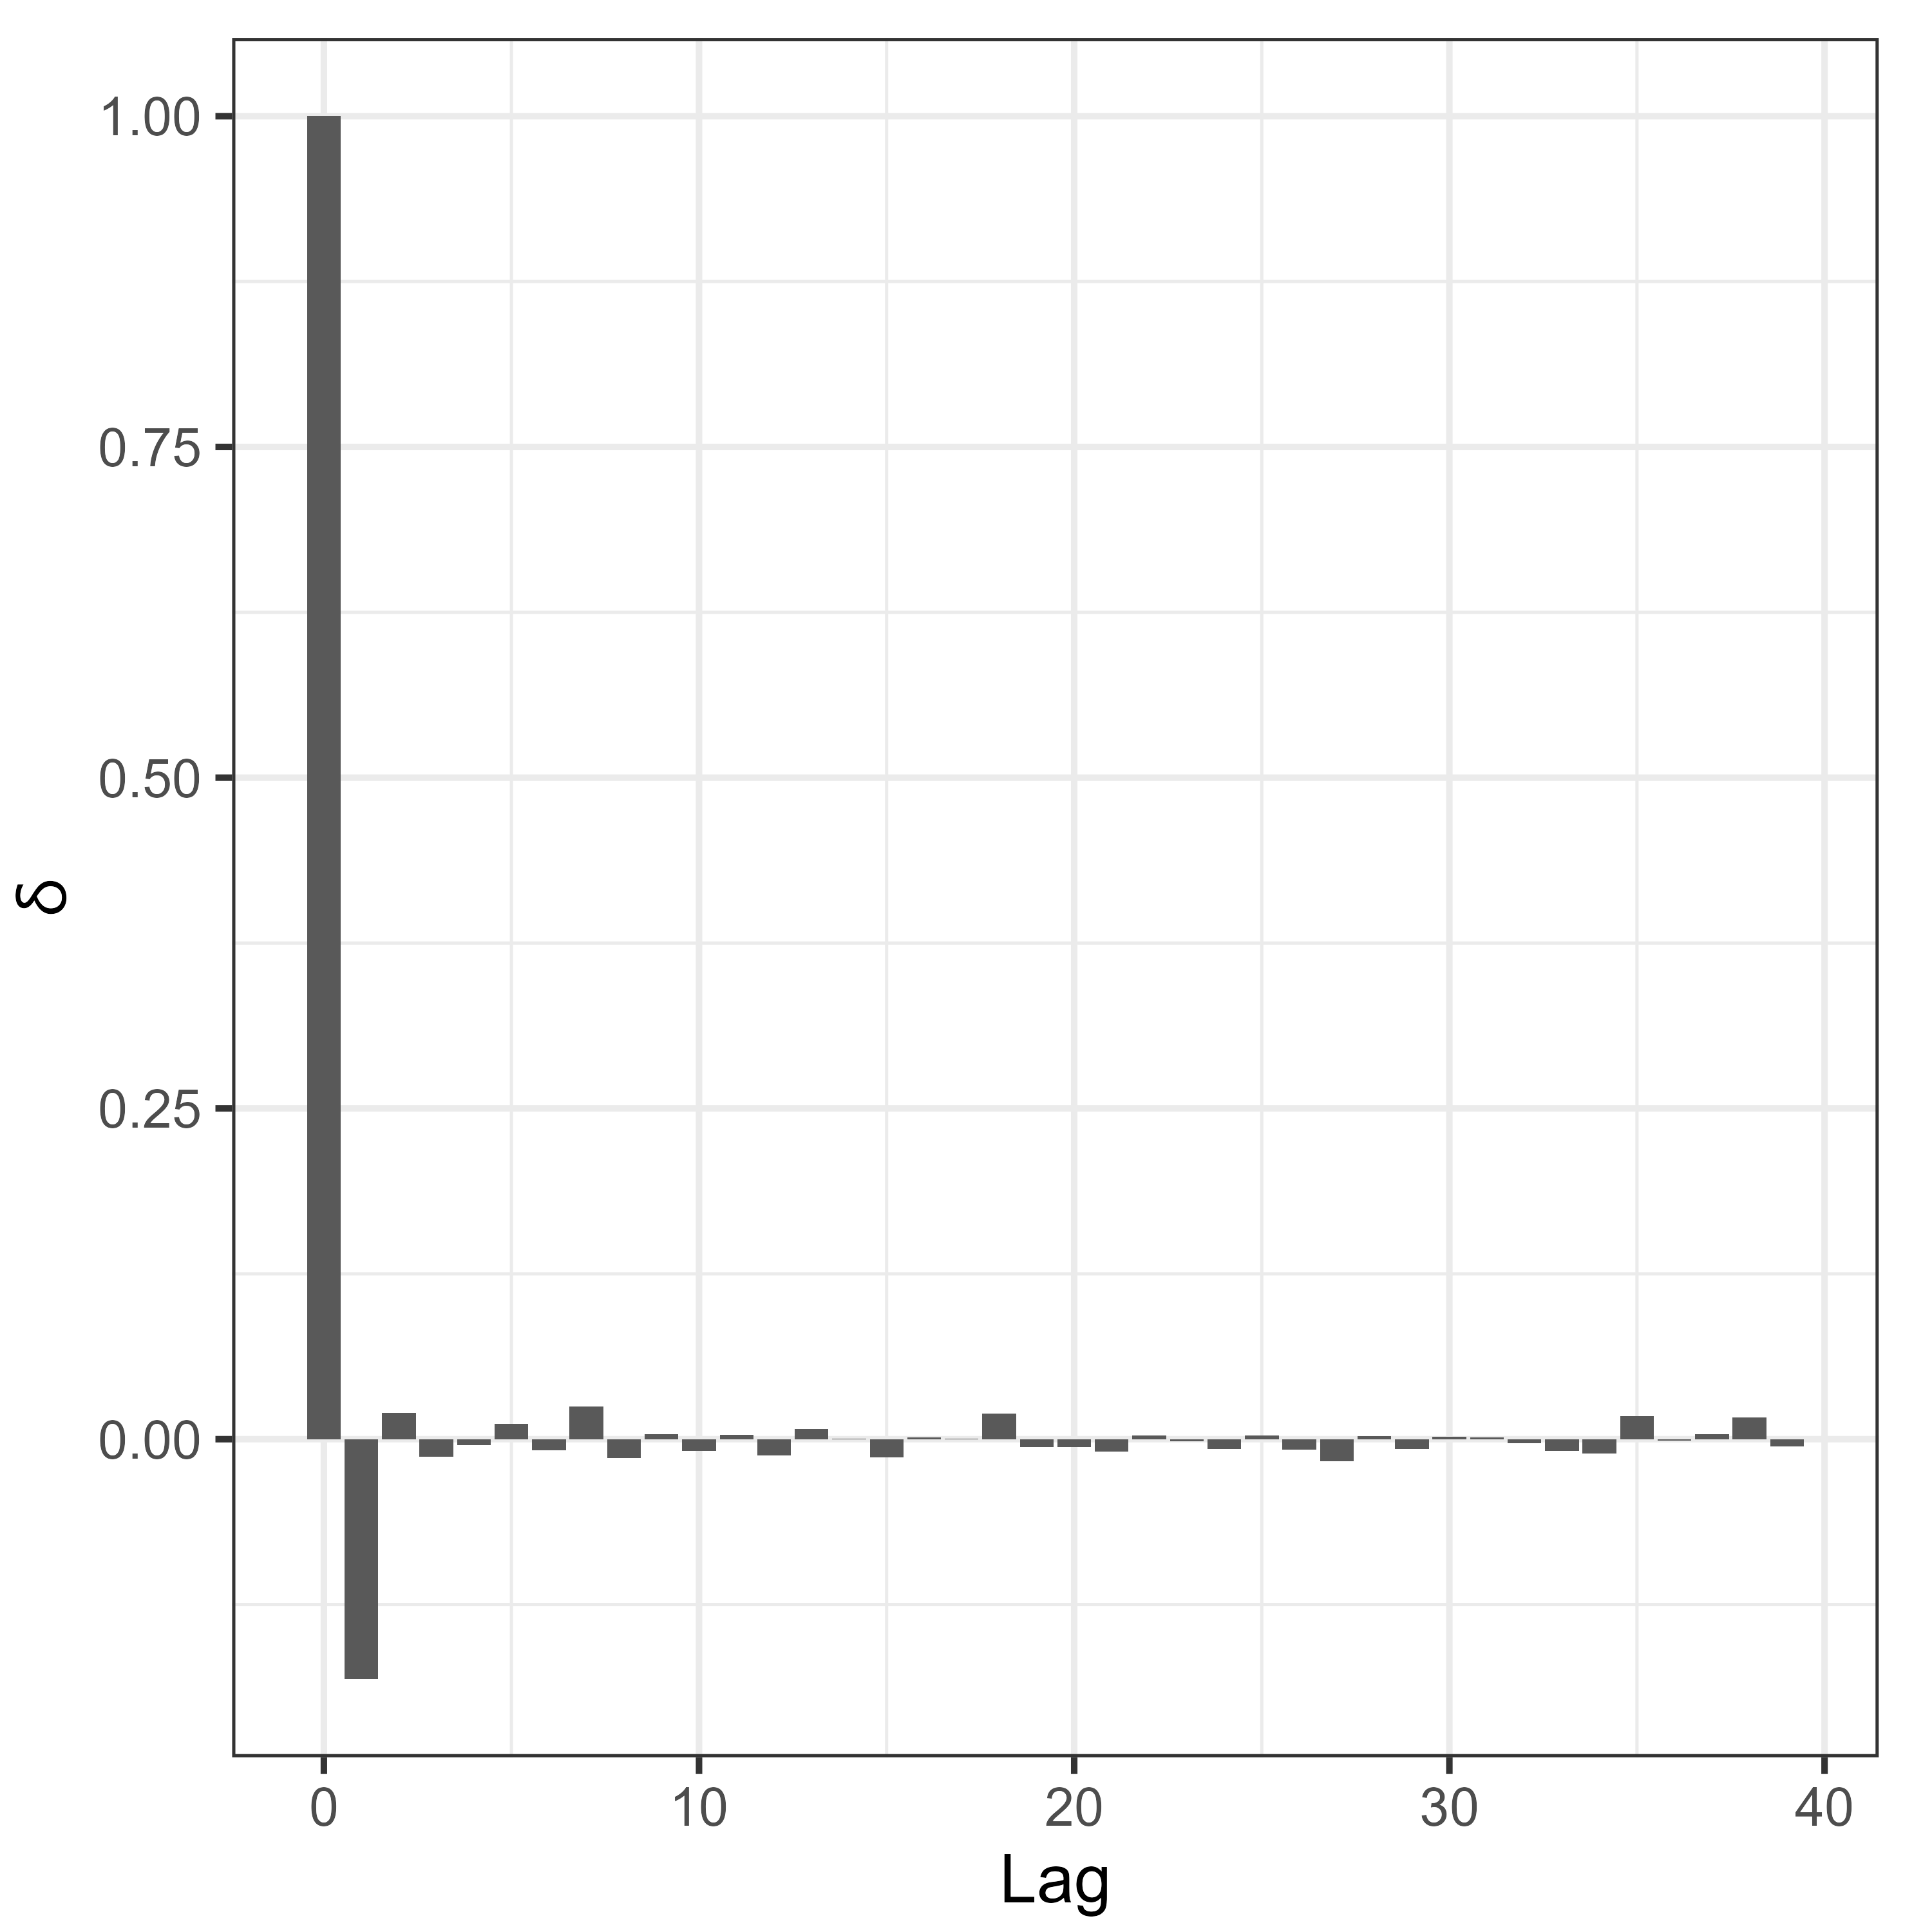
\includegraphics[width=0.8\textwidth]{../figures/acemoglu/hist_beta.png}
\caption{Posterior Distribution of $\beta$ --- Replication Study}
\label{fig:replication_posterior_distributions}
\end{figure}

As shown, our Bayesian model closely recovers the frequentist point estimates reported by \cite{acemogluColonialOriginsComparative2001} when assuming strict exclusion. This provides reassuring evidence that, under the exclusion restriction, the Bayesian and frequentist approaches align.

However, one of the main advantages of the Bayesian framework is that it naturally accommodates departures from strict exclusion. By allowing for a nonzero $\gamma$, with a prior centered at zero but with increasing variance, we can examine how the posterior inference on $\beta$ changes. 

The sensitivity analysis presented in Figure \ref{fig:replication_sensitivity_analysis} shows how varying the prior variance for $\gamma$ affects the posterior distribution of $\beta$. When the prior variance is very small, we essentially recover the frequentist estimate; as the prior variance increases, the posterior mean of $\beta$ decreases, and the credible intervals widen, reflecting increased uncertainty about the exclusion restriction.

\begin{figure}[H]
    \centering
    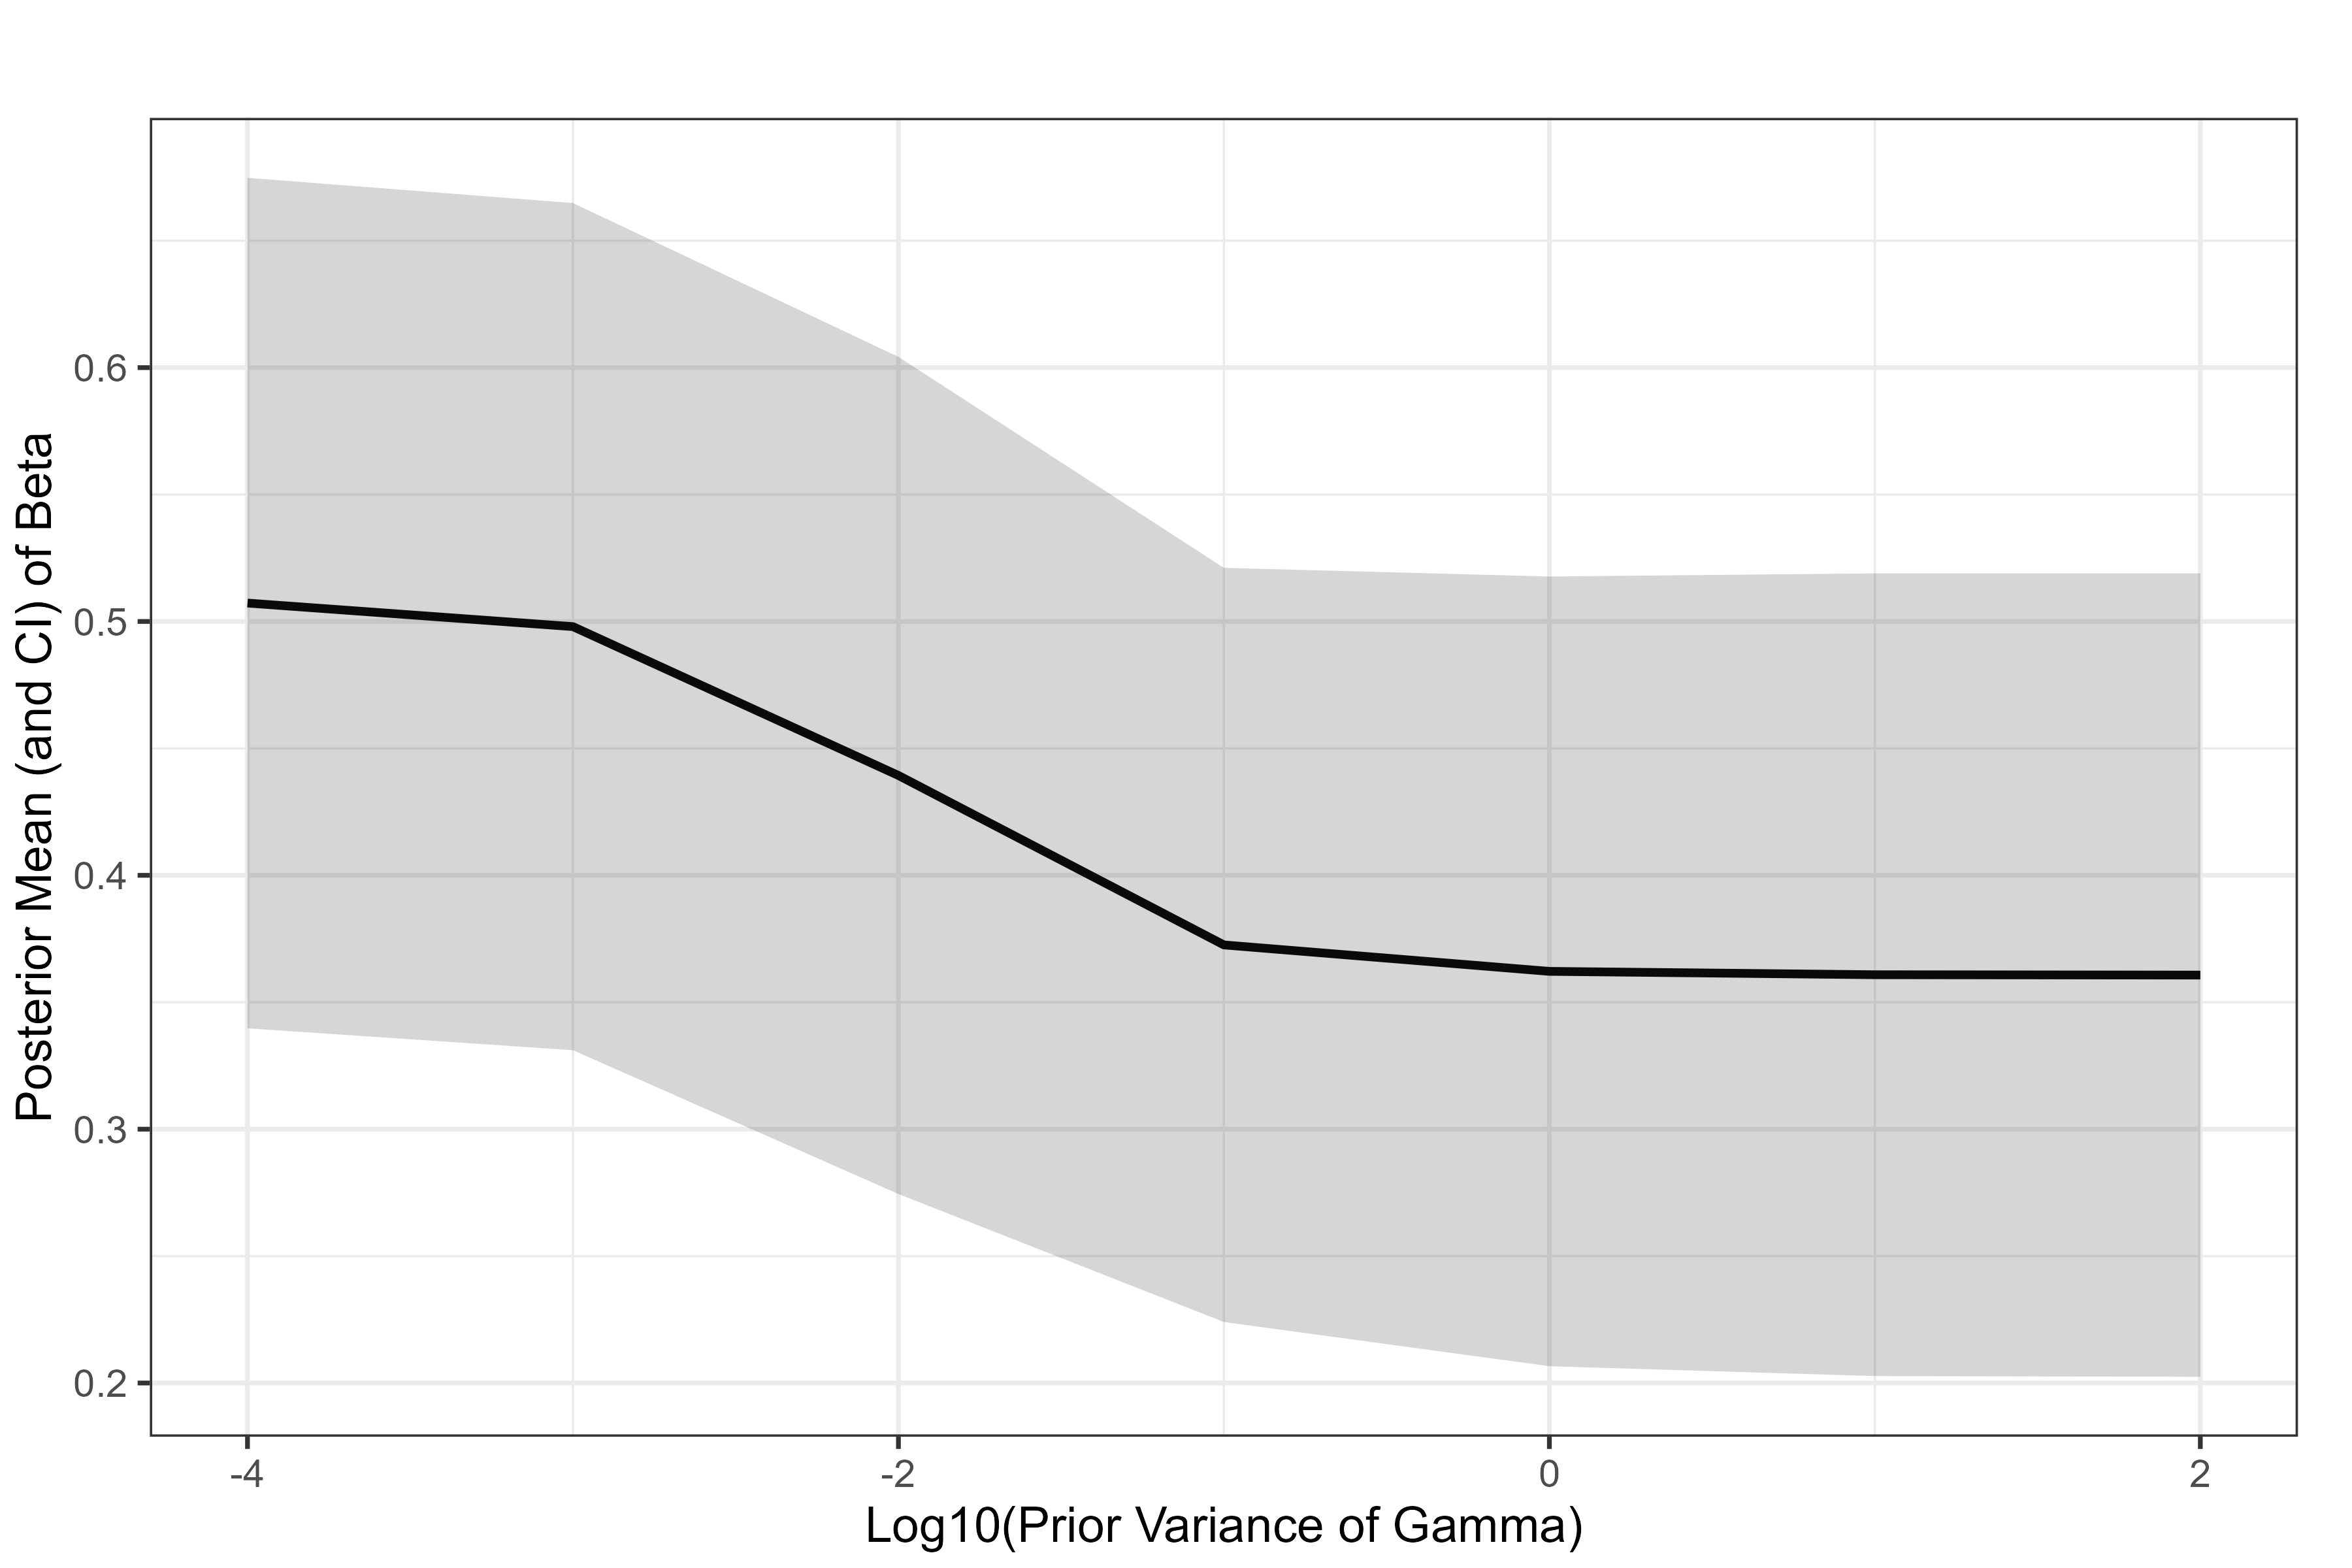
\includegraphics[width=0.9\textwidth]{../figures/acemoglu/plot_prior_gamma.png}
    \caption{Sensitivity Analysis of $\widehat{\beta}$ to Prior Variance of $\gamma$ --- Replication Study}
    \label{fig:replication_sensitivity_analysis}
    \end{figure}

It is important to note that in this specific case, even with a wide prior variance, we do not lose statistical significance of the coefficient on $\beta$. Nonetheless, in settings where significance could be lost, \cite{conleyPlausiblyExogenous2012} provide a Bayesian solution to a sensitivity analysis problem, but do not offer a direct method to incorporate the substantive expertise of the researcher regarding the likely magnitude of $\gamma$.

To address this gap, \cite{vankippersluisPlausiblyExogenous2018} propose an extension. They build upon the strategy suggested by \cite{angristWhyWorldWar1994}, who advocated examining subsamples where the first stage is weak or null. If the exclusion restriction holds, the reduced form should also show no significant relationship in these subsamples. 

\cite{vankippersluisPlausiblyExogenous2018} adapt this idea to the Bayesian framework: for observations where the first-stage effect is weak, they use the estimated reduced form coefficient to inform a prior for the direct effect $\gamma$. If the reduced form in such subsamples is significantly different from zero, it suggests a violation of exclusion, and this information is incorporated into the prior for $\gamma$.

However, this approach requires assuming homogeneous treatment effects, even though heterogeneous effects are likely present, particularly when the first-stage relationship varies across subsamples. Additionally, selecting the appropriate subsample is nontrivial and must be done carefully to avoid introducing further biases.

\bigskip

In summary, we review the approaches of \cite{conleyPlausiblyExogenous2012} and \cite{vankippersluisPlausiblyExogenous2018} to account for possible violations of the exclusion restriction within a Bayesian framework. We apply these methods to simulated datasets and to the empirical context of \cite{acemogluColonialOriginsComparative2001}. We find that the Bayesian plausibly exogenous approach not only recovers the frequentist estimates under strict exclusion but also provides a powerful and flexible tool for sensitivity analysis when the validity of the instrument is questionable.
 

% --- Bibliography --

\bibliographystyle{chicago}
\bibliography{references}

\end{document}
